\documentclass[a4paper, openright, 12pt]{report}
\usepackage[a4paper, left=40mm, right=25mm, top=30mm, bottom=25mm]{geometry}
\usepackage[spanish, english]{babel} % espanol
\usepackage{graphicx} % graficos
\usepackage{subcaption}
\usepackage{longtable}
\usepackage{sectsty}
\usepackage{titlesec}
\usepackage{multirow}
\usepackage{ragged2e}
\usepackage{enumerate}
\usepackage{graphicx}
\usepackage{url}
\usepackage{listings}
\usepackage{tocloft}
\usepackage[hidelinks]{hyperref}
\graphicspath{ {images/} }

\chapternumberfont{\small} 
\chaptertitlefont{\small}

\titleformat*{\section}{\small\bfseries}
\titleformat*{\subsection}{\small\bfseries}

\addto\captionsenglish{
\renewcommand{\chaptername}{Capítulo}
\renewcommand{\appendixname}{Apéndice}
\renewcommand{\contentsname}{Índice}
\renewcommand{\listfigurename}{Índice de figuras}
\renewcommand{\listtablename}{Índice de cuadros}
\renewcommand{\tablename}{Cuadro}	
\renewcommand{\figurename}{Figura}	
\renewcommand{\bibname}{Bibliografía}	
}

\begin{document}
\begin{titlepage}

\begin{figure}[h]
\captionsetup{justification=centering,margin=2cm}

\includegraphics[scale=1]{escudoUta}
\centering
\end{figure}
\begin{center}
\textbf{UNIVERSIDAD TÉCNICA DE AMBATO}
\end{center}
\begin{center}
\textbf{FACULTAD DE INGENIERÍA EN SISTEMAS, ELECTRÓNICA E INDUSTRIAL}
\end{center}
\begin{center}
\textbf{CARRERA DE INGENIERÍA EN SISTEMAS COMPUTACIONALES E INFORMÁTICOS}
\end{center}
\begin{center}
TEMA:
\end{center}
\begin{center}
\rule{150mm}{0.1mm}
\end{center}
\begin{center}
DESARROLLO DE UN VIDEOJUEGO 2D PARA LA ENSEÑANZA DE LA CULTURA Y MITOLOGÍA INCA
\end{center}
\begin{center}
\rule{150mm}{0.1mm}
\end{center}
\begin{center}
Trabajo de Graduación Modalidad: Proyecto de Investigación, presentado previo la obtención del título de Ingeniero en Sistemas Computacionales e Informáticos
\end{center}
\begin{center}
SUBLÍNEA DE INVESTIGACIÓN:
\end{center}
\begin{center}
Orientación a objetos
\end{center}
\begin{center}
AUTOR: Carlos José Acuña Aguaguiña\\
TUTOR: Ing. Franklin Mayorga, Mg
\end{center}
\begin{center}
Ambato - Ecuador\\
Abril, 2020
\end{center}
\end{titlepage}

\pagenumbering{roman}
\setcounter{page}{2}
\newpage
\chapter*{APROBACIÓN DEL TUTOR}
\addcontentsline{toc}{chapter}{APROBACIÓN DEL TUTOR}
En mi calidad de Tutor del Trabajo de Investigación sobre el tema: ``DESARROLLO DE UN VIDEOJUEGO 2D PARA LA ENSEÑANZA DE LA CULTURA Y MITOLOGÍA INCA", del señor Carlos José Acuña Aguaguiña, estudiante de la Carrera de Ingeniería en Sistemas Computacionales e Informáticos, de la Facultad de Ingeniería en Sistemas, Electrónica e Industrial de la Universidad Técnica de Ambato, considero que el informe investigativo reúne los requisitos suficientes para que continúe con los trámites y consiguiente aprobación de conformidad con el numeral 7.2 de los Lineamientos Generales para la aplicación de Instructivos de las Modalidades de Titulación de las Facultades de la Universidad Técnica de Ambato.
\begin{flushright} 
Ambato, abril de 2020
\end{flushright}
\vfill
\begin{center}
Ing. Franklin Mayorga, Mg\\
EL TUTOR
\end{center}
\newpage
\chapter*{AUTORÍA}
\addcontentsline{toc}{chapter}{AUTORÍA}
El presente trabajo de investigación titulado: ``DESARROLLO DE UN VIDEOJUEGO 2D PARA LA ENSEÑANZA DE LA CULTURA Y MITOLOGÍA INCA" Es absolutamente original, auténtico y personal, en tal virtud, el contenido, efectos legales y académicos que se desprenden del mismo son de exclusiva responsabilidad del autor.
\begin{flushright} 
Ambato, abril de 2020
\end{flushright}
\vfill
\begin{center}
Carlos José Acuña Aguaguiña\\
CC: 1804413373
\end{center}
\newpage
\chapter*{DERECHOS DE AUTOR}
\phantomsection
\addcontentsline{toc}{chapter}{DERECHOS DE AUTOR}
Autorizo a la Universidad Técnica de Ambato, para que haga uso de este Trabajo de Titulación como un documento disponible para la lectura, consulta y procesos de investigación.\\
Cedo los derechos de mi Trabajo de Titulación, con fines de difusión pública además autorizo su reproducción dentro de las regulaciones de la Universidad.
\begin{flushright} 
Ambato, abril de 2020
\end{flushright}
\vfill
\begin{center}
Carlos José Acuña Aguaguiña\\
CC: 1804413373
\end{center}
\newpage
\chapter*{Aprobación del tribunal de Grado}
\phantomsection
\addcontentsline{toc}{chapter}{Aprobación del tribunal de Grado}
\newpage
\chapter*{Dedicatoria}
\phantomsection
\addcontentsline{toc}{chapter}{Dedicatoria}
\hfill
\begin{minipage}{0.45\textwidth}
\begin{tabular}{p{\textwidth}}
Dedicado a mi familia por todo su apoyo y consideración.\\
\bigskip
A la Facultad de Ingeniería en Sistemas\\ Electrónica e Industrial.\\
\bigskip
Gracias totales.
\end{tabular}
\end{minipage}
%
\begin{flushright}
\vfill
Carlos José Acuña Aguaguiña
\end{flushright}
\newpage
\chapter*{Agradecimiento}
\phantomsection
\addcontentsline{toc}{chapter}{Agradecimiento}
\hfill
\begin{minipage}{0.45\textwidth}
\begin{tabular}{p{\textwidth}}
Agradezco a mi familia por apoyarme en todos los momentos y darme la oportunidad de prepararme y ser una mejor persona en todos los aspectos de la vida.
\end{tabular}
\end{minipage}
%
\begin{flushright}
\vfill
Carlos José Acuña Aguaguiña
\end{flushright}
\newpage
%
%
\tableofcontents
\clearpage
\listoffigures
\clearpage
\listoftables
%
%
\newpage
\chapter*{Resumen Ejecutivo}
\phantomsection
\addcontentsline{toc}{chapter}{Resumen Ejecutivo}
\justify
En el mundo han existido una gran número de civilizaciones que han moldeado la sociedad, entre ellas se encuentra la cultura Inca, la cual ha heredado costumbres y tradiciones que se han transmitido de generación en generación a través de mitos y leyendas.\\
\justify
Gracias a los videojuegos se puede crear verdaderas obras maestras que no solo entretengan al espectador sino también le den un mensaje, una enseñanza que le sirva para conocer mejor un tema, en este caso una civilización que existió hace mucho tiempo y que tuvo un gran impacto en el desarrollo de la sociedad latinoamericana y ecuatoriana.\\
\justify
A nivel nacional el desarrollo de videojuegos es un campo no muy explorado y por lo tanto no se toma enserio el potencial educativo que tienen, han existido varios intentos de desarrollo pero solo han sido relegados a pequeños proyectos universitarios y trabajos independientes.\\
\justify
El presente videojuego fue desarrollo en Unity3D con el lenguaje de programación C\#, y para el diseño se utilizó el programa GIMP.
\justify
Se utilizó la metodología ágil conocida como DAV propuesta por por Gabriel Armendáriz estudiante de la facultad de Informática de la EPOCH (Escuela Superior Politécnica de Chimborazo).
\justify
Los resultados obtenidos después de la publicación del videojuego en la plataforma Gamejolt fueron favorables debido al número de vistas y descargas realizadas por los usuarios pese a ser un juego independiente con una temática educativa de fondo.

\newpage
\chapter*{Abstract}
\phantomsection
\addcontentsline{toc}{chapter}{Abstract}
In the world there have been a large number of civilizations that have shaped society, among them is the Inca culture, which has inherited customs and traditions that have been transmitted from generation to generation through myths and legends.\\
\justify
Thanks to video games you can create true masterpieces that not only entertain the viewer but also give them a message, a teaching that will help them better understand a subject, in this case a civilization that existed a long time ago and that had a great impact in the development of Latin American and Ecuadorian society.\\
\justify
At the national level the development of video games is a not very explored field and therefore the educational potential they have is not taken seriously, there have been several attempts at development but they have only been relegated to small university projects and independent work.\\
\justify
This video game was developed in Unity3D with the C\# programming language, and the GIMP program was used for the design.\\
\justify
The agile methodology known as DAV proposed by Gabriel Armendáriz, student of the Computer Science faculty of EPOCH (Escuela Superior Politécnica de Chimborazo) was used.\\
\justify
The results obtained after the publication of the video game on the Gamejolt platform were favorable due to the number of views and downloads made by users despite being an independent game with a background educational theme.

\newpage
\chapter*{INTRODUCCIÓN}
\phantomsection
\addcontentsline{toc}{chapter}{Introducción}
\justify
El presente proyecto de investigación denominado ``DESARROLLO DE UN VIDEOJUEGO 2D PARA LA ENSEÑANZA DE LA CULTURA Y MITOLOGÍA INCA" se encuentra divido en los siguientes capítulos.
\bigskip
\justify
CAPÍTULO I. ``MARCO TEÓRICO'', plantea un problema el cual se ha de investigar y se busca una justificación para realizar esta investigación además de definir objetivos que guiarán el desarrollo de este proyecto.
\bigskip
\justify
CAPÍTULO II. ``METODOLOGÍA", reúne todas las técnicas e instrumentos necesarios para obtener, procesar y analizar los datos obtenidos, además, define las etapas para el desarrollo del presente proyecto.
\bigskip
\justify
CAPÍTULO IV. ``RESULTADOS Y DISCUSIÓN", se indica de manera clara y concisa el desarrollo del proyecto, así como la comparación de las mejores metodologías y frameworks que permitan el desarrollo del videojuego.
\bigskip
\justify
CAPÍTULO V. ``CONCLUSIONES Y RECOMENDACIONES", en este apartado se señalan algunas conclusiones y recomendaciones que se han encontrado a lo largo del desarrollo del proyecto.
\newpage
\setcounter{page}{1}
%%%%%%%%%%%%%%%%%%%%%%%%%%%%%%%%%CAPITULO 1%%%%%%%%%%%%%%%%%%%%%%%%%%%%%%%%%%%%%%
\chapter{Marco Teórico}
\pagenumbering{arabic} % para empezar la numeración con números
\section{Tema de investigación}
\justify
Desarrollo de un videojuego 2D para la enseñanza de la cultura y mitología inca.

\section{Antecedentes investigativos}

\subsection{Contextualización del problema}
\justify
En el mundo han existido un gran número de civilizaciones que han moldeado la sociedad y han heredado sus conocimientos, hallazgos, costumbres y tradiciones para el futuro de la humanidad. Gracias a la compleja conectividad de la glo-balización con ayuda de las tecnologías de información y comunicación es posible conocer cada rincón del mundo y por lo tanto descubrir muchas de estas culturas que han sido inmortalizadas en el consciente colectivo de la gente mediante obras literarias, películas, series de televisión e incluso videojuegos \cite{tomlinson2013}. Es así como ahora se conoce civilizaciones tan antiguas como la griega y su mitología en torno a dioses como Zeus, Poseidón, Hades entre otros \cite{grimal1991}, o la cultura vikinga y su mitología nórdica con su propio panteón de ases como Odín, Thor y Loki \cite{alvarez2002}. Esto ha permitido que los descendientes de estas civilizaciones se sientan orgullosos de sus ancestros y tengan bien definido sus raíces.\\
Mucho de esta contribución para conocer la historia antigua ha sido en gran medida gracias a la industria de los videojuegos donde se puede destacar varios títulos muy importantes como son GOD OF WAR, un juego que tiene mecánicas de peleas con varios oponentes que se relacionan con la mitología griega y los principales dioses y monstruos de este panteón, además, este  juego toma lugar en lugares reales del planeta y donde el jugador puede sumergirse más profundamente en esta cultura \cite{mobygames2005}. Otro título muy conocido es el juego AGE OF MITOLOGY donde el principal objetivo es ganar a las demás naciones militarmente a través de la evolución de su tecnología, desarrollo de la economía y pidiendo el favor de los dioses. El juego se basa en culturas ricas en cultura y mitología y donde las leyendas de héroes y dioses son contadas de manera ingeniosa y donde el jugador se puede sentir parte de la historia \cite{mobygames2003}.\\
Sin embargo, esa misma globalización, encabezada por la masiva explosión cultural de Estados Unidos alrededor del mundo está causando que otros países pierdan sus costumbres y tradiciones y se olviden de sus raíces culturales\cite{Boundless2019}. Además, existen naciones que tratan de rescatar su cultura mediante varios proyectos gubernamentales, así tenemos al gobierno francés que subsidia la producción nacional cinematográfica y obliga a los teatros y cines a estrenar películas de origen francés cada cierto tiempo \cite{VargasLlosa2000}.\\
Otra nación que protege su cultura a pesar de la influencia anglosajona es México, donde el estado se preocupa de mantener sus costumbres y tradiciones, a salvo, y hay casos donde su propia gente decide hacer algo al respecto, así tenemos a un joven ilustrador, Pedro Ramírez Lara, que realiza ilustraciones donde los protagonistas son dioses de la época prehispánica de México con el fin de dar a conocer las leyendas, cuentos y mitología de su cultura \cite{Mulato2016}.\\
Así mismo, un grupo de jóvenes peruanos han creado un cómic sobre las aventuras de los hermanos Ayar, que son parte de las leyendas de mitología inca y una muestra de que la mitología Sudamericana es rica en historias y leyendas \cite{Andina2019}. En el Ecuador este tipo de iniciativas no se ha visto apoyada o mencionada en ninguna parte por lo tanto la gente olvida su identidad cultural y prefiere adoptar costumbres extranjeras.

\subsection{Delimitación}
\begin{flushleft}
\textbf{Área Académica:} Software\\
\textbf{Línea de investigación:} Desarrollo de software\\
\textbf{Sublíneas de investigación:} Orientación a objetos\\
\textbf{Delimitación especial:} Este proyecto no está delimitada a una área geográfica, ya que busca ser publicada en una tienda virtual, por lo tanto su dimensión es a nivel global\\
\textbf{Delimitación temporal:} La presente investigación se desarrollará durante los
6 meses posteriores a la aprobación del proyecto por parte del Consejo Directivo
de la Facultad que constituye desde el mes de diciembre de 2019 hasta - junio de 2020.
\end{flushleft}

\subsection{Justificación}
\justify
La importancia de esta investigación se fundamenta en elevar el interés de las personas por la historia nacional y conocer las raíces de todos los ecuatorianos mediante el uso de herramientas tecnológicas, que en este caso son conocidos como videojuegos, ya que busca rescatar las costumbres y tradiciones de los pueblos autóctonos del país, centrándose en la región andina; siendo un proyecto original ya que busca crear una experiencia diferente para los usuarios. Aquí el beneficiario final son las futuras generaciones del país, especialmente los estudiantes y personas que quieran conocer sobre la maravillosa historia del Ecuador.

\section{Fundamentación teórica}
\justify
Como parte inicial se debe conocer el concepto de videojuego, que según el diccionario de la Real Academia Española (RAE) lo define como “Juego electrónico que se visualiza en una pantalla, o un dispositivo electrónico que permite, mediante mandos apropiados, simular juegos en las pantallas de un televisor, una computadora u otro dispositivo electrónico” \cite{Espanola2019}. Sin embargo, se puede encontrar una definición más profunda a cargo de Ana Laura Rossaro en su artículo “Aprender jugando: Los videojuegos y su potencial educativo” quien dice que “… en general los videojuegos recrean entornos y situaciones en los que el jugador (o varios jugadores) pueden controlar personajes e interactuar con el entorno para alcanzar un objetivo determinado…” \cite{Rossaro2012}.\\
Es así como un videojuego puede tener tantos enfoques como situaciones a explorar, pero en este trabajo se toma particular atención al campo educativo y su impacto en la sociedad ecuatoriana, como resultado se encontraron varios proyectos de este tipo con el fin de entregar un producto que tenga un valor adicional y sirva como ayuda en el aprendizaje de algún tema en particular.\\
Al realizar una búsqueda de otros proyectos de videojuegos a nivel nacional enfocados en la educación se ha encontrado títulos muy interesantes y que vale la pena mencionar, como son: \\
El proyecto de Hussein Gabriel Rahman Núñez de la Universidad Técnica de Ambato, que para el 2007, creó un videojuego enfocado en la informática donde los movimientos del personaje se interpretan mediante comandos básicos de lógica de programación lo que permite conocer y entender cómo funcionan la mayoría de los videojuegos y las ciencias computacionales desde un punto de vista distinto al método tradicional de educación teniendo unos resultados favorables al momento de publicar el juego en la plataforma ``Game Jolt" con más de 1000 descargas \cite{RahmanNunez2017}.
También se encuentra el programa creado por Alejandro Pardina Bustamante de la Escuela Politécnica Nacional en 2017 donde su enfoque fue mejorar el trabajo en equipo utilizando un videojuego multijugador, comprobando que se mejoró las capacidades colaborativas de las personas que se atrevieron a probar el juego \cite{PardinaBustamante2016}.\\
Con estos ejemplos se puede conocer que los videojuegos pueden ser utilizados como herramientas de aprendizaje haciendo que sus usuarios aprendan algo nuevo mientras resuelven problemas y se entretienen.\\ 
En este proyecto se busca crear un videojuego que cumpla con la misma función de enseñar a la gente sobre la cultura y mitología de los pueblos incas en el Ecuador; es lamentable saber que no se ha tratado de realizar un videojuego basado en este tema ya que la historia de los ancestros del país es rica y multidiversa y por lo tanto se puede considerar un primer paso para conocer mejor las costumbres y tradiciones autóctonas del Ecuador.\\
La presente investigación se enmarca en el paradigma Crítico Propositivo, es crítico porque realiza un Análisis Crítico del problema, y es Propositivo porque busca proponer una solución factible al problema.\\
Según el plan nacional del Buen Vivir de la constitución de la República del Ecuador en el Art. 293 en el numeral 2.3 se encuentra “Promover el rescate, reconocimiento, investigación y protección del patrimonio cultural, saberes ancestrales, cosmovisiones y dinámicas culturales.” De esta manera se cumple con la ley y se beneficia a la nación y a la cultura ecuatoriana.

\justify
Entre los términos más utilizados y de los cuales se basa la presente investigación son:

\justify
\textbf{Periodo prehispánico.} Dicho de América o de lo relacionado con ella: Anterior a la conquista y colonización españolas \cite{Espanola2119}.\\
\textbf{Civilizaciones de América Latina.} En la américa precolombina existieron grandes civilizaciones como la civilización olmeca, los mayas, los quiches, culturas del Valle de México, la civilización peruana de Norte Chico y el imperio inca \cite{chang2007}.\\
\textbf{Imperio inca.} Fundadores de uno de los imperios más grandes de la historia de la humanidad, el cual fue conocido como el Tahuantinsuyo ocupaba un territorio de más de 4000 Km y tenía una población de cerca de 12 millones de habitantes reinaron el cono sur de América hasta su declive en el siglo XVI \cite{baudouin2012}.\\
\textbf{Cultura y mitología inca ecuatoriana.} La cultura inca estaba llena de costumbres, tradiciones y dioses a los cuales sus pobladores adoraban fervientemente para recibir bendiciones, especialmente para sus cosechas. En el panteón Inca se muestra la imagen de Viracocha, dios de la creación, Inti, dios del sol, Mama quilla, diosa de la luna, Pachamama o madre tierra entre otros seres mitológicos y héroes que hicieron hazañas que se cuentan hasta hoy en día \cite{steele2004}.\\
\textbf{Informática.} Ciencia encargada de estudiar y desarrollar máquinas para tratar y transmitir información, así como, los métodos para procesarla. Y también se puede decir que es un conjunto de conocimientos tanto teóricos como prácticos sobre cómo se construyen, funcionan y utilizan las computadoras \cite{de2004}.\\
\textbf{Programación.} “ Es el proceso por medio del cual se diseña, codifica, limpia y protege el código fuente de programas computacionales. A través de la programación se dictan los pasos a seguir para la creación del código fuente de programas informáticos. De acuerdo con ellos el código se escribe, se prueba y se perfecciona ” \cite{programacion2019}.\\
\textbf{Videojuegos.} El concepto de Johan Huizinga es utilizado tanto en juego reales como virtuales y dice. “El juego es una actividad libre y consciente que ocurre fuera de la vida ‘ordinaria’ porque se considera que no es seria, aunque a veces absorbe al jugador intensa y completamente. […] Promueve la formación de grupos sociales que tienden a rodearse a sí mismos de secreto y a acentuar sus diferencias respecto del resto utilizando los medios más variados” \cite{lacasa2011}. \\
\textbf{Videojuegos 2D.} Es un tipo de videojuego de 2 dimensiones donde se debe tomar en cuenta las colisiones de los cuerpos como en la vida real, este sistema de detección de colisiones es habitualmente un módulo que ayuda a crear acciones para los objetos dentro del videojuego \cite{moyadesarrollo}.

\section{Objetivos}
\subsection{General}
\begin{itemize}
\item Desarrollar un videojuego 2D, enfocado en la enseñanza de las costumbres y mitología inca ecuatoriana.
\end{itemize}

\subsection{Específicos}
\begin{itemize}
\item Investigar las costumbres, tradiciones y mitología del pueblo inca.
\item Seleccionar un motor gráfico para el desarrollo de videojuegos.
\item Utilizar una metodología ágil que se adapte al desarrollo de videojuegos.
\item Implementar el videojuego en 2D enfocado en la enseñanza de las costumbres y mitología inca ecuatoriana.
\end{itemize}
%%%%%%%%%%%%%%%%%%%%%%%%%%%%%%%%%CAPITULO 2%%%%%%%%%%%%%%%%%%%%%%%%%%%%%%%%%%%%%%
\chapter{Metodología}
\section{Métodos}
\subsection{Modalidad de la investigación}
\begin{itemize}
\item \textbf{Investigación Bibliográfica}\\
La investigación será bibliográfica ya que se apoyará en libros, revistas, tesis del área de informática, documentos técnicos, trabajos de titulación del área de ciencias humanas y arte cuentos, leyendas y leyes existentes para la elaboración del marco teórico que se divide en dos partes fundamentales; la historia, costumbres y tradiciones del pueblo inca en el Ecuador y los videojuegos.

\item \textbf{Investigación de modalidad especial}\\
Al ser una investigación que se centra en un aspecto social se le considera de modalidad especial porque busca, mediante una solución tecnológica, contribuir al desarrollo cultural del país y rescatar costumbres y tradiciones propias de esta tierra.
\end{itemize}

\subsection{Población y muestra}
\justify
El presente proyecto no tiene una población específica ya que su dimensión es global y busca llegar a la mayor cantidad de gente posible.

\subsection{Procesamiento y análisis de datos} 
\justify
Se debe empezar por recopilar información sobre la cultura y mitología inca, paralelamente a esto, investigar sobre los motores de juegos y metodologías ágiles que permitan el desarrollo del proyecto.

\subsection*{Historia general de la cultura inca}
\justify
A principios del siglo XIII apareció una tribu indígena de lengua quechua cerca de Cuzco que enseguida adoptó el nombre de su líder: Inca. A pesar de tener dificultades para adaptarse al nuevo territorio tuvo que acoger las costumbres de los pueblos cercanos pero sin abandonar su idioma original. La historia narrada oralmente de los Incas comienza con el primer inca, Manco Cápac.\\
Se establecieron en el interior de los Andes del Perú Meridional, en la cuenca de Cuzco, cerca de los ríos Huaytanay y Tullumayo, una región ocupada por otras tribus. Después de varios batallas que duraron alrededor de dos siglos el único pueblo que quedaba era el inca, lo que hizo que se convirtiera en uno de los imperios más grandes que ha conocido la humanidad.\\
Luego de varios conquistas más allá de su territorio llegó a anexar pueblos formando así el el Tahuantinsuyo, que ocupó una vasta superficie, extendiéndose a lo largo del territorio de las actuales repúblicas del Perú, Ecuador, Bolivia, Argentina, Chile y el sur de Colombia.\cite{baudouin2012incas}

\begin{figure}[h]
\captionsetup{justification=centering,margin=2cm}
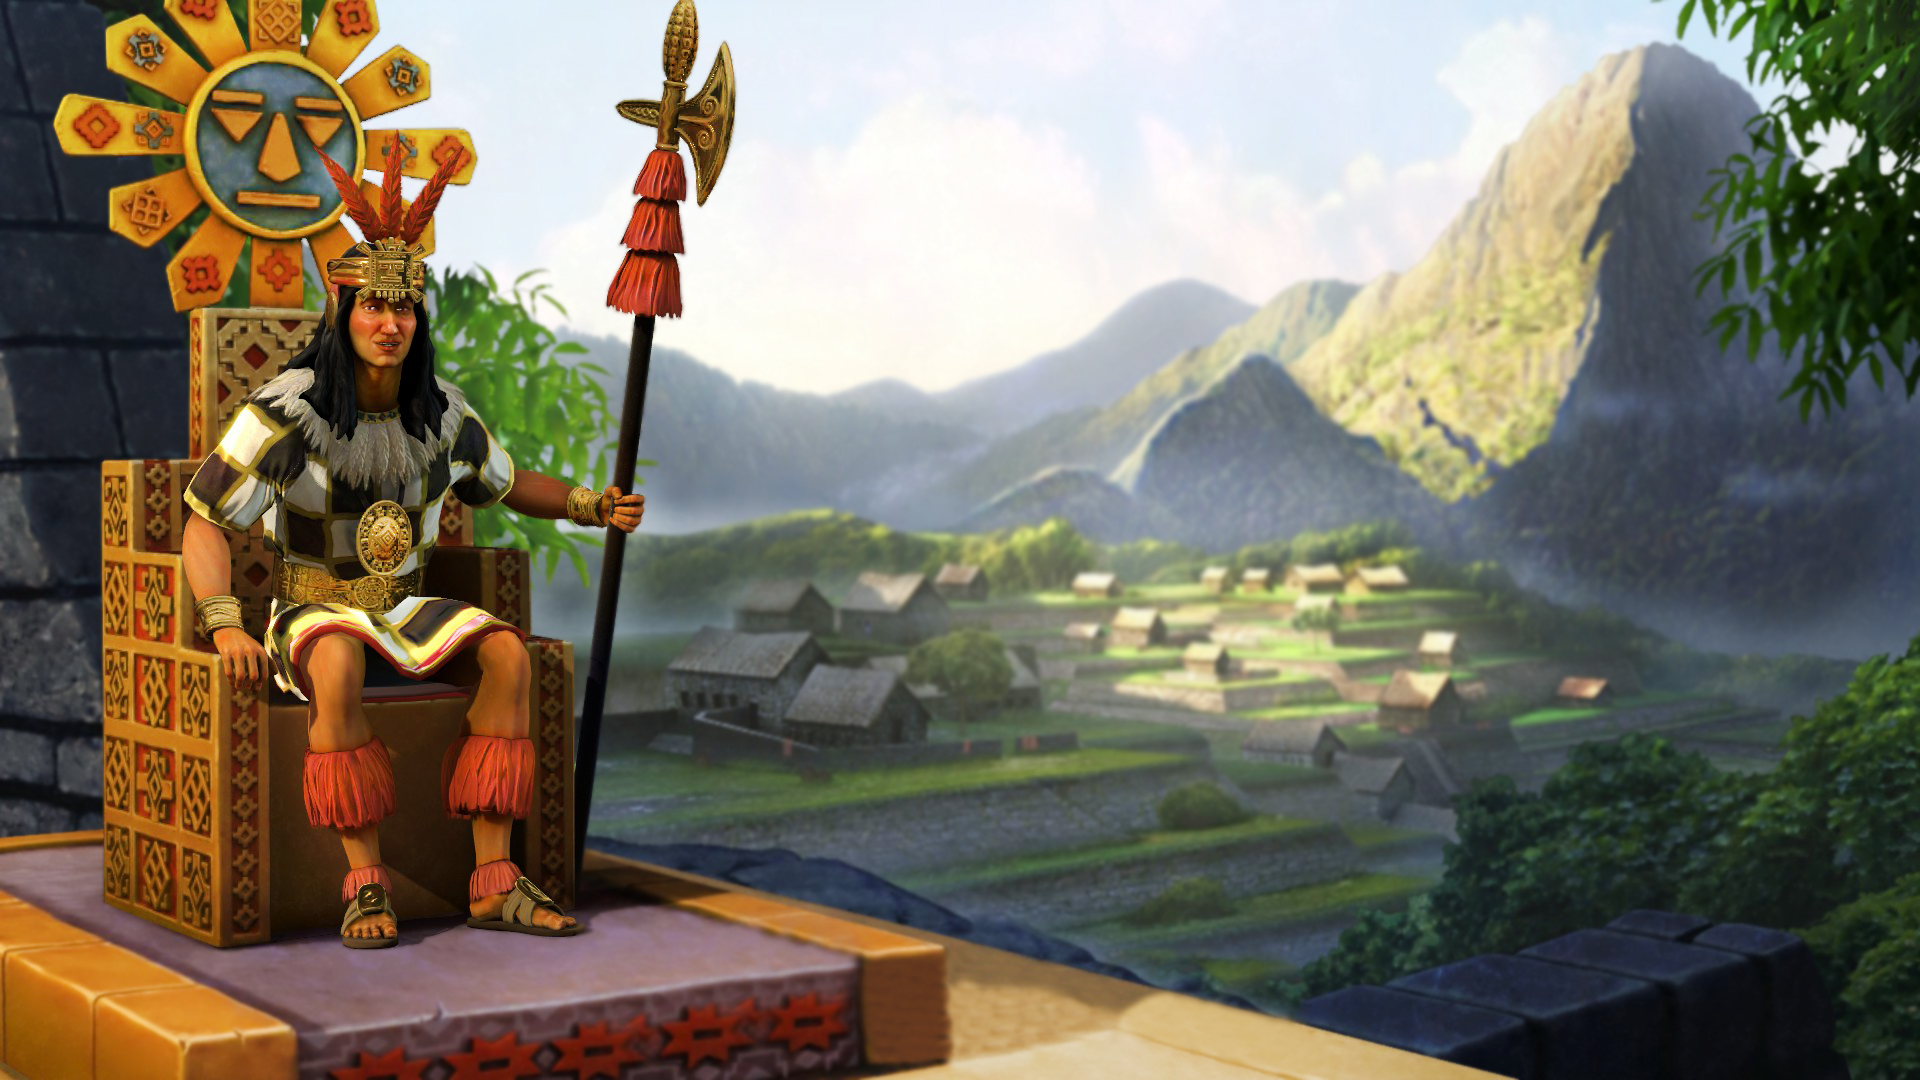
\includegraphics[scale=0.2]{h1}
\centering
\caption{Imperio Inca}
Elaborado por: Carlos Acuña
\label{fig:h1}
\end{figure}
  
\subsection*{Personajes principales}
\subsection*{Huaynacápac}
\justify
Huayna Cápac fue el undécimo y antepenúltimo inca del Tahuantinsuyo. Emperador del Cuzco. No está claro el lugar de su nacimiento, se estima nacido en Cuzco, aunque se discute si probablemente nació en Tomebamba, actual ciudad de Cuenca. Hijo del Sapa Inca Túpac Yupanqui y de la Coya Mama Ocllo, nacido durante las expediciones de conquista emprendidas por su padre durante el reinado de Pachacútec. Durante su infancia y juventud fue llamado Titu Cusi Huallpa.
Túpac Yupanqui enfermó en Chinchero, eligiendo como su sucesor al menor de sus hijos, hecho que disgustó a algunas panacas cuzqueñas que esperaban que el sucesor fuera Cápac Guari hijo de la concubina Chuqui Ocllo. Gracias a la oportuna intervención de su tío materno Huamán Achachi la conspiración no prosperó y fue nombrado Inca tomando el nombre de Huayna Cápac, Con un inicio tan agitado empezó el gobierno del nuevo Inca, que básicamente tuvo que dedicar todos sus esfuerzos a consolidar los terrenos conquistados por su padre y sofocar las revueltas de provincias levantiscas. Para esto, asumió el control político y religioso del Imperio, desplazando a Apo Chalco Yupanqui, el vigente Villac Umo. Por primera vez en la época imperial se concentraban todos los poderes en una sola persona. Sin embargo, casi al final de su vida nombra un pariente suyo, Cusi Túpac Yupanqui, como nuevo Sumo Sacerdote del Sol (aparentemente este es el Villac Umo que corona a Manco Inca y que lo secundaría en sus guerras de reconquista como hábil estratega).
Antes de su muerte, alrededor del año 1525 dividió su imperio entre sus hijos Atahualpa y Húascar y fue conocido como uno de los mejores líderes de todos los tiempos junto a su padre y abuelo. \cite{de2006enciclopedia}

\begin{figure}[h]
\captionsetup{justification=centering,margin=2cm}
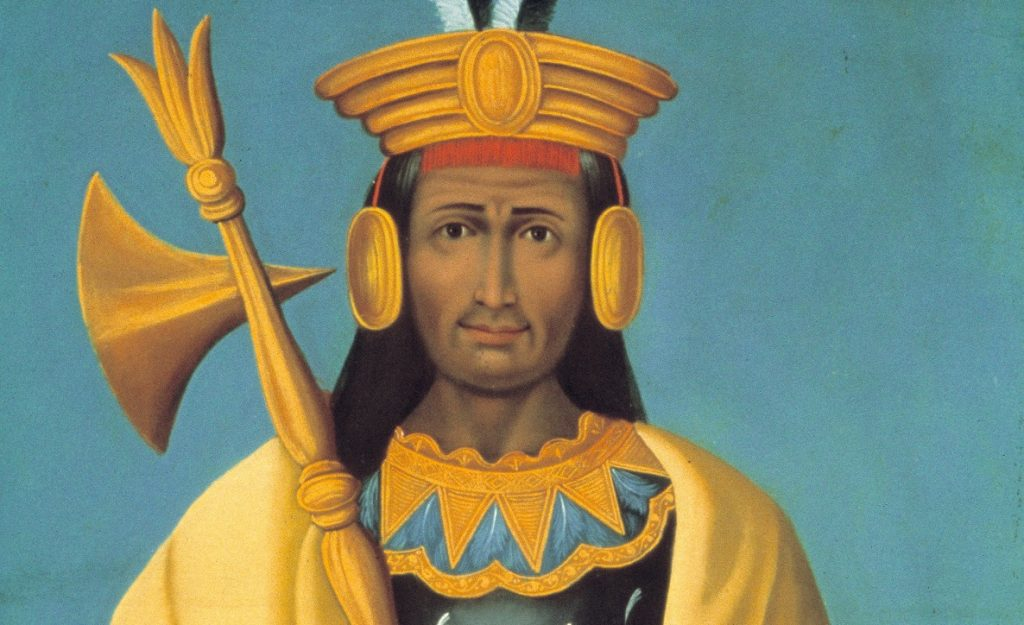
\includegraphics[scale=0.4]{h2}
\centering
\caption{Huaynacápac}
Elaborado por: Carlos Acuña
\label{fig:h2}
\end{figure}
\clearpage
\subsection*{Atahualpa}
\justify
Hijo de la princesa shyri Pacha y del rey inca Huaynacápac o (Huayna - Cápac), atahualpa es el fruto de la sangrienta conquista inca en nuestro país. Nació en Quito probablemente en 1497. Durante un tiempo vivió en paz junto a su padre y no tuvo conflictos, al menos bélicos, con su medio hermano Húascar. La división del reino hecha por su padre propició la guerra entre los dos hermanos. Cómo líder militar tomó sabias decisiones. Durante las batallas contra su medio hermano supo aprovechar las victorias y manejar bien las derrotas. Con sus enemigos fue implacable. Cuando llegaron los invasores españoles no quiso aceptar la fé católica ni el bautismo y fue condenado. Pagaron por su rescate, pero fue en vano. El último emperador inca murió el 26 de julio de 1533. Su pueblo afirmó qu en ese momento anocheció a mitad del día. \cite{2010batallas}

\begin{figure}[h]
\captionsetup{justification=centering,margin=2cm}
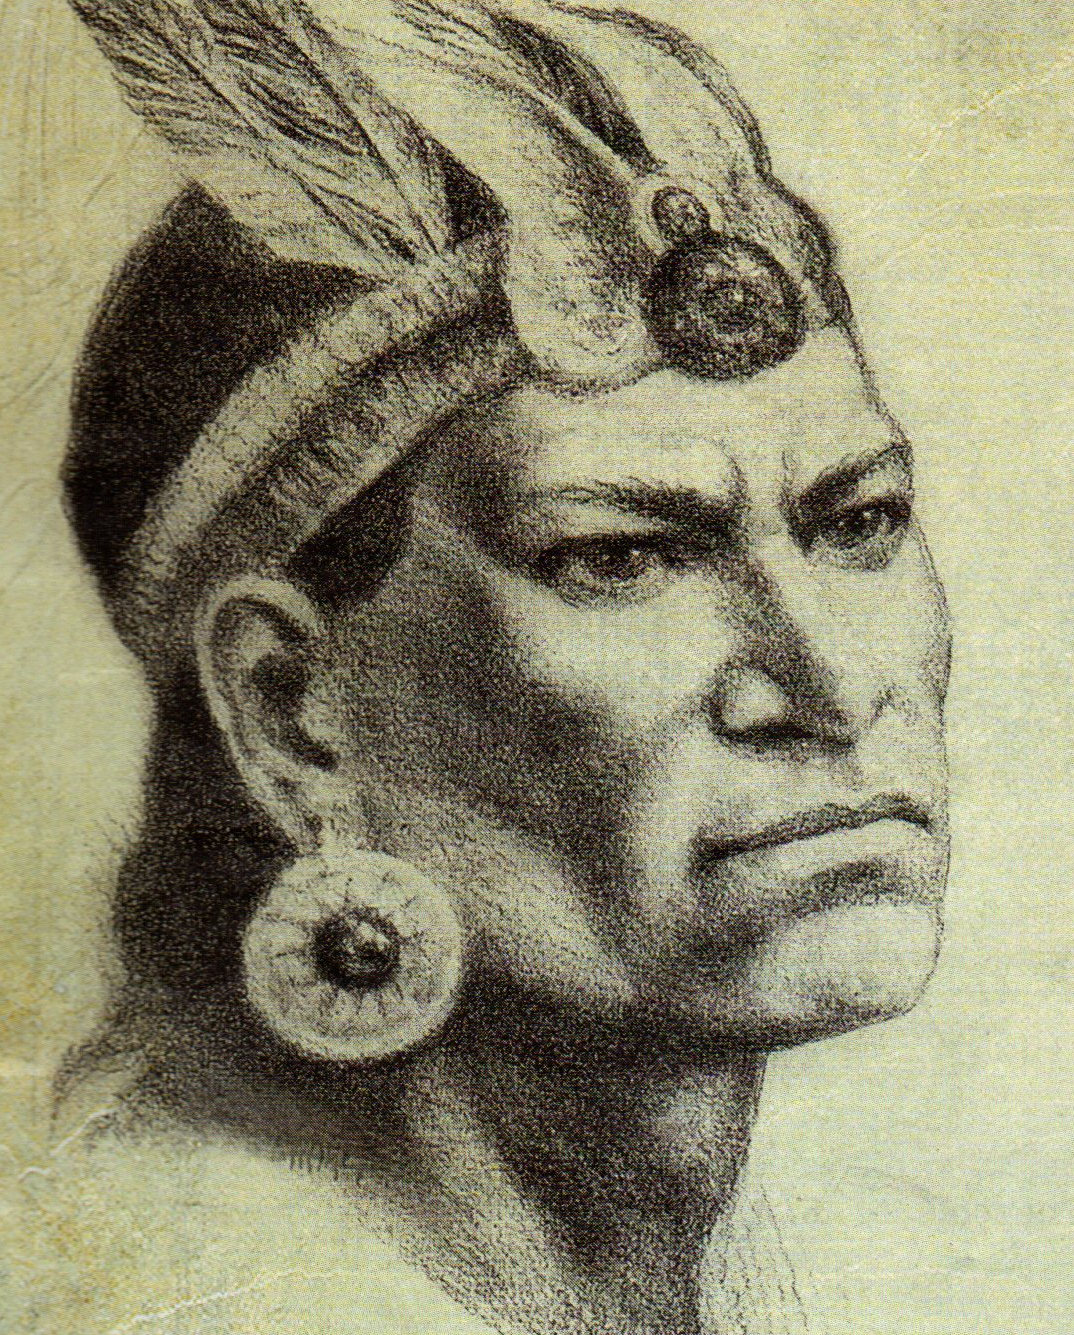
\includegraphics[scale=1]{h3}
\centering
\caption{Atahualpa}
Elaborado por: Carlos Acuña
\label{fig:h3}
\end{figure}
\clearpage
\subsection*{Huáscar}
\justify
Primogénito de Huaynacápac o (Huayna - Cápac), y Araua Ocllo. Nació en el Cuzco, alrededor de 1491. Huáscar era de linaje inca puro. Esto era muy importante en el Tahuantinsuyo, pues se creía que los incas de sangre pura descendían directamente de la divinidad. Jamás aceptó que su medio hermano Atahualpa gobierne junto a él, así que, influido por la nobleza cuzqueña, decidió atacarlo. Aunque envió varios contingentes , perdió  muchas batallas y no pudo detener la avanzada de los ejércitos del norte quienes por órdenes de Atahualpa decidieron tomarse la capital, el Cuzco. Fue aprisionado Quisquis. Su captura significó la victoria definitiva de Atahualpa. Murió tiempo después de ser capturado y encerrado en la fortaleza de Jauja. \cite{2010batallas}

\begin{figure}[h]
\captionsetup{justification=centering,margin=2cm}
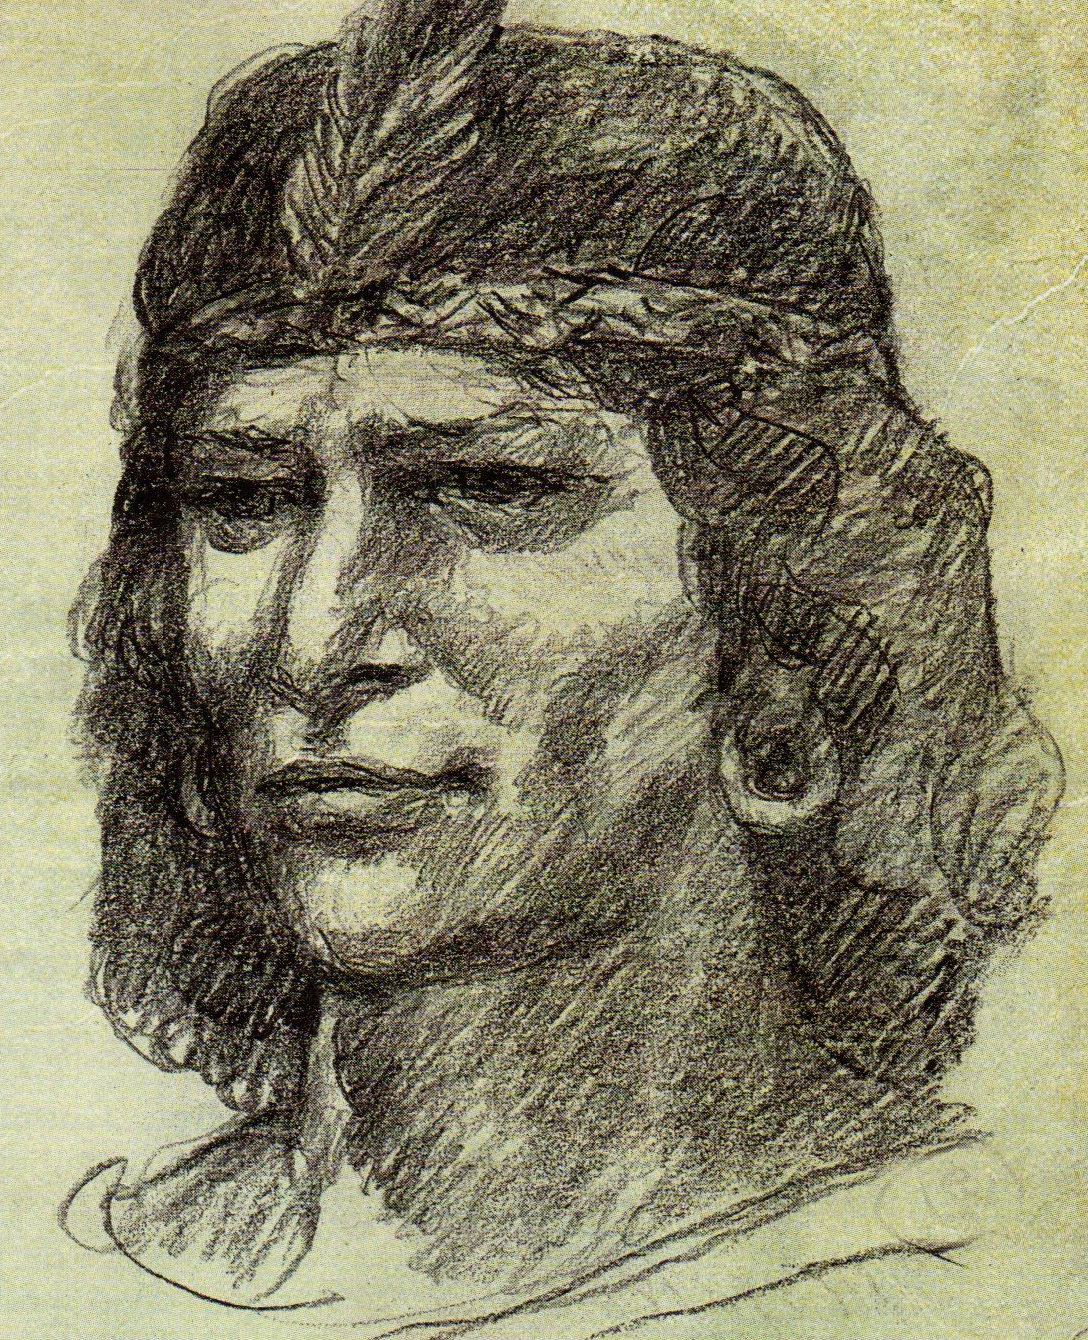
\includegraphics[scale=1]{h4}
\centering
\caption{Huáscar}
Elaborado por: Carlos Acuña
\label{fig:h4}
\end{figure}
\clearpage
\subsection*{Quisquis}
\justify
Destacado general inca. Según algunos biógrafos, su nombre significa pequeña ave. Estuvo bajo las órdenes de Huaynacápac; después de su muerte, permaneció al lado de Atahualpa. Tuvo triunfos y derrotas frente a las tropas de Huáscar, pero en Quipaipán elaboró una brillante estrategia para capturar al líder cuzqueño. Después de que los españoles llegaron y atahualpa fuera encarcelado, Quisquis o (Quis-quis) opuso resistencia a los españoles, enfrentándolos y capturando a varios de ellos. Intentó crear una reunificación inca para defenderse de los invasores pero no lo consiguió. Fue asesinado por sus propios capitanes, al no poder convencerlo de rendirse ante los españoles. \cite{2010batallas}

\begin{figure}[h]
\captionsetup{justification=centering,margin=2cm}
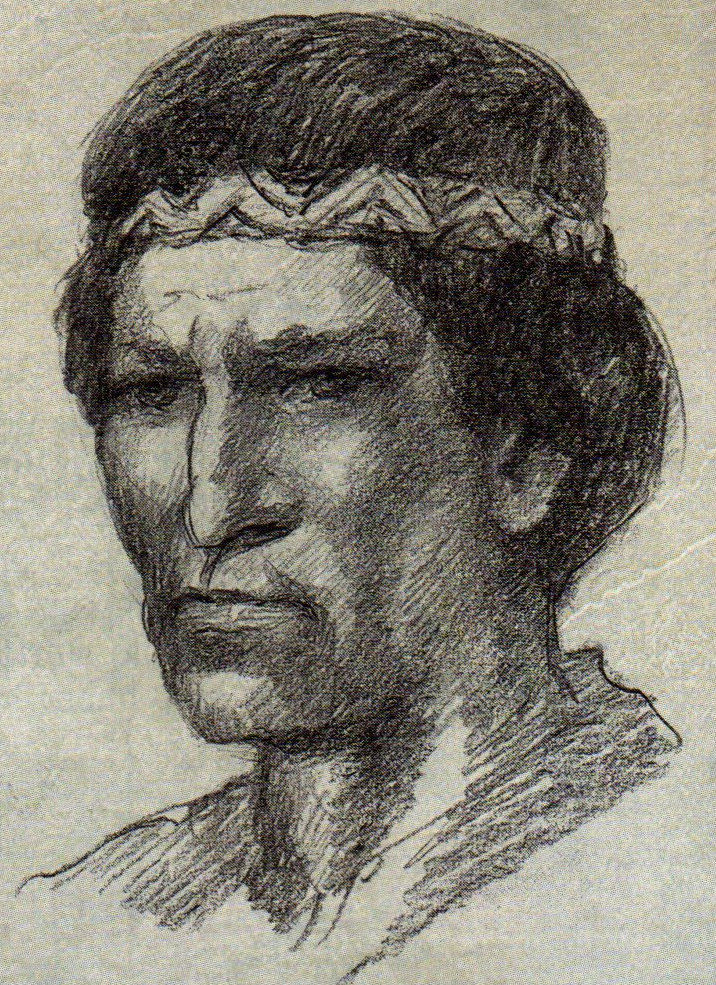
\includegraphics[scale=1]{h5}
\centering
\caption{Quisquis}
Elaborado por: Carlos Acuña
\label{fig:h5}
\end{figure}

\clearpage
\subsection*{Calicuchima}
\justify
Hijo de Epiclachima y comandante de los ejércitos de Atahualpa. Luego de perder las primeras batallas ante los invasores del Cuzco, preparó junto a Quisquis ofensiva meditada. Aislaron al ejército de Huáscar y lo llevaron al territorio del norte para tenderle una emboscada en Molleambato. Mediante esa estrategia obtienen la primera de varias victorias frente a los guerreros del Sur. Participó en la captura de Huáscar. Fue Calicuchima quien supuestamente entregó el oro de rescate que los invasores españoles pedían por Atahualpa. Fue condenado a muerte debido a que mantenía correspondencia con Quisquís, quien se declaró en rebeldía. \cite{2010batallas}

\begin{figure}[h]
\captionsetup{justification=centering,margin=2cm}
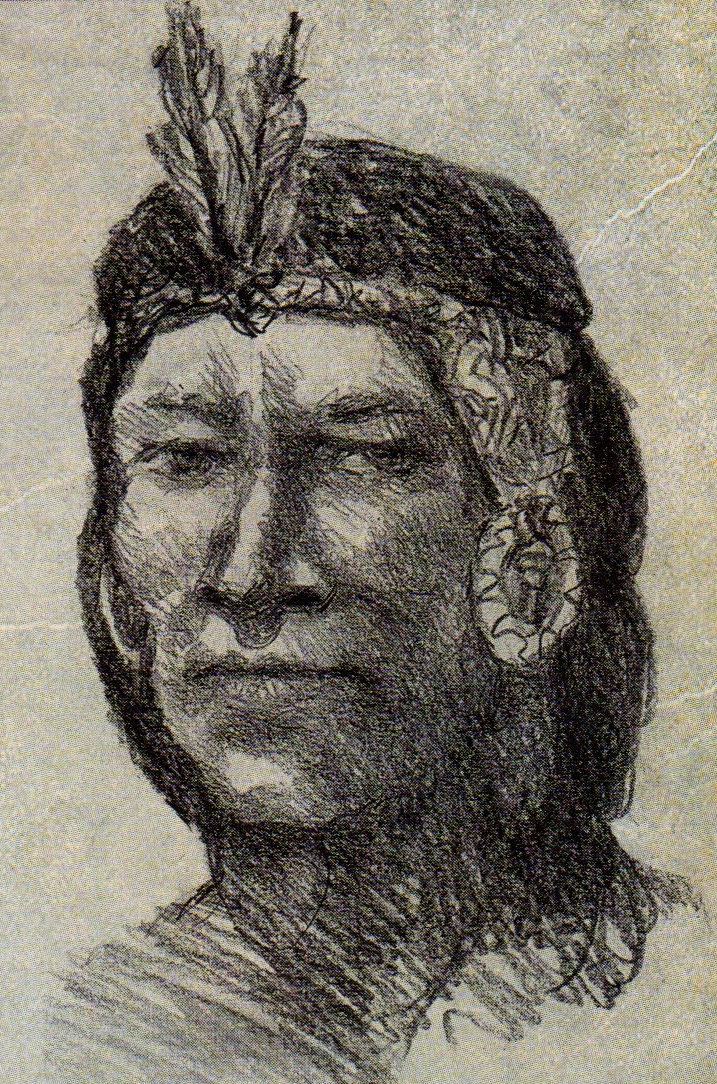
\includegraphics[scale=1]{h6}
\centering
\caption{Calicuchima}
Elaborado por: Carlos Acuña
\label{fig:h6}
\end{figure}

\clearpage
\subsection*{Chapera}
\justify
Cacique del reino Cañari. No quiso someterse a Atahualpa y renegó de él para aliarse con Húascar. Avanzó junto a Apu Atoc con el fin de de derrotar a Atahualpa. Fue capturado en la batalla de Molleambato. Posteriormente fue ejecutado en Quito. Su pueblo sufrió la violencia de Atahualpa por haber sido traicionado. \cite{2010batallas}

\begin{figure}[h]
\captionsetup{justification=centering,margin=2cm}
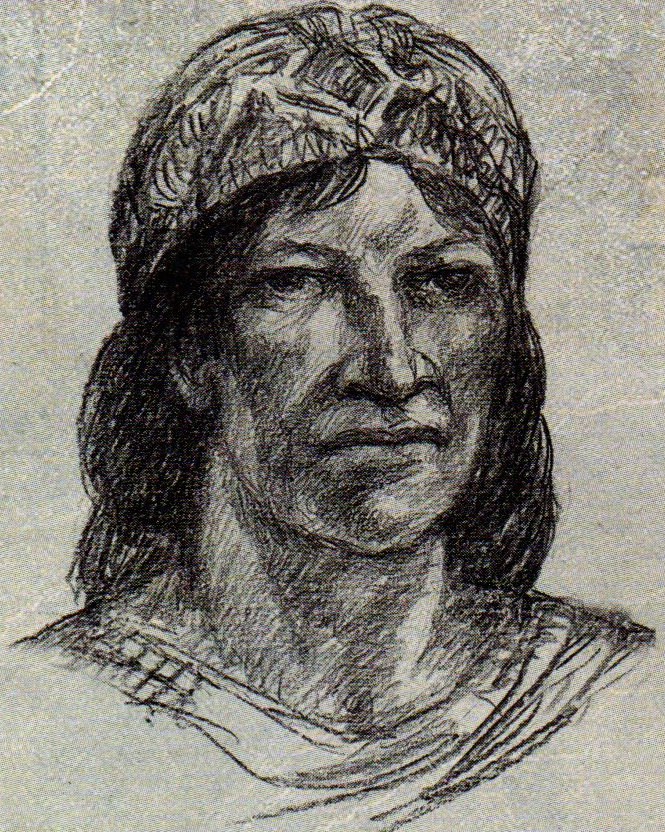
\includegraphics[scale=0.8]{h7}
\centering
\caption{Chapera}
Elaborado por: Carlos Acuña
\label{fig:h7}
\end{figure}

\subsection*{Apu Atoc}
\justify
Capitán al mando del ejército de Huáscar. Aunque sus primeras incursiones por el territorio del norte fueron exitosas, sus contingentes fueron los en sufrir la derrota de los ejércitos de Atahualpa. Fue capturado en la batalla de Molleambato y ejecutado en Quito por las órdenes de Rumiñahui. \cite{2010batallas}

\begin{figure}[h]
\captionsetup{justification=centering,margin=2cm}
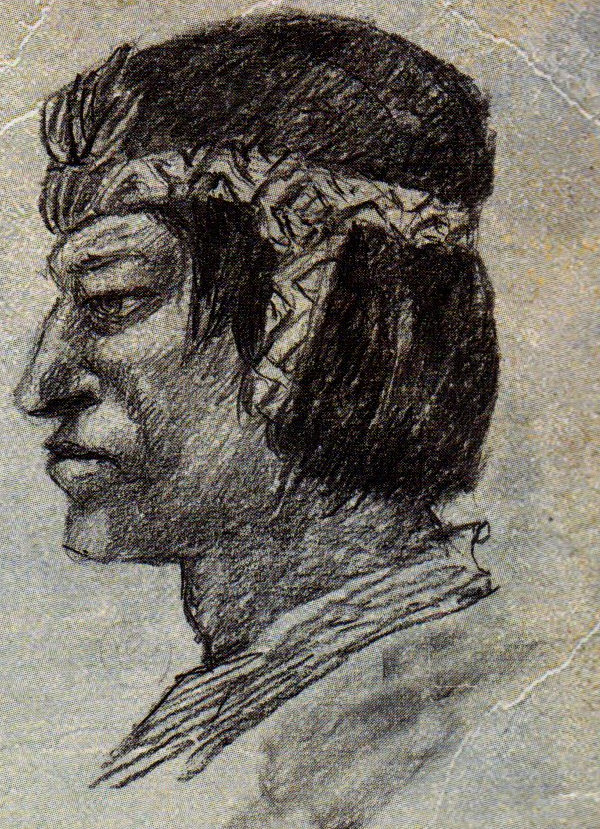
\includegraphics[scale=0.8]{h8}
\centering
\caption{Apu Atoc}
Elaborado por: Carlos Acuña
\label{fig:h8}
\end{figure}
\clearpage
\subsection*{Batallas principales}
\subsection*{Batalla de Molleambato}
\justify
\textbf{Antecedentes.} El conquistador inca Huaynacápac cumplió con la misión de unificar el imperio inca a través de numerosas batallas. Cuando llegó su vejez decidió heredar el Tahuantinsuyo a sus descendientes. Húascar se quedó con el Cuzco, mientras que Atahualpa hijo de Paccha, princesa de los quitus, heredó el norte. El pueblo de Cuzco , al no estar satisfecho con la división realizada se alió con los cañaris para destronar al heredero del norte. Atoc general de Huáscar, avanzó hasta el dominio cañari para aliarse con ellos. Al llegar su ejército desplazó a los guerreros del norte, quienes ofrecieron poca resistencia. Con el fin de detener la avanzada, Atahualpa, decide viajar a la comarca de Ambatus.\cite{2010batallas}\\  
\textbf{El enfrentamiento.} Atoc, quien dirigía la avanzada de Huáscar, decide descansar con su ejército entre Mocha y Ambato, con el fin de esperar refuerzos. Mientras tanto, los hombres de Atahualpa se movilizan a la orilla opuesta del río Ambato y esperan el ataque del adversario, quien tiene que cruzar el río para llegar hasta ellos.\\
El general Calicuchima, del ejército quiteño, con 5000 hombres, rodea las montañas occidentales y llega a Quisapincha (sur de Ambato) e inicia una ofensiva desde el sur.
Las fuerzas de Atahualpa aprovechan la confusión entre las tropas sureñas y vadean el río para atacar desde el norte. Los cuzqueños fueron derrotados. La batalla fue tan sangrienta que el historiador Federico Gonzáles Suárez afirma que años más tarde los conquistadores hallaron el campo blanqueado debido a la cantidad de huesos no sepultados. Los sobrevivientes se refugiaron en Tomebamba. \cite{2010batallas}

\begin{figure}[h]
\captionsetup{justification=centering,margin=2cm}
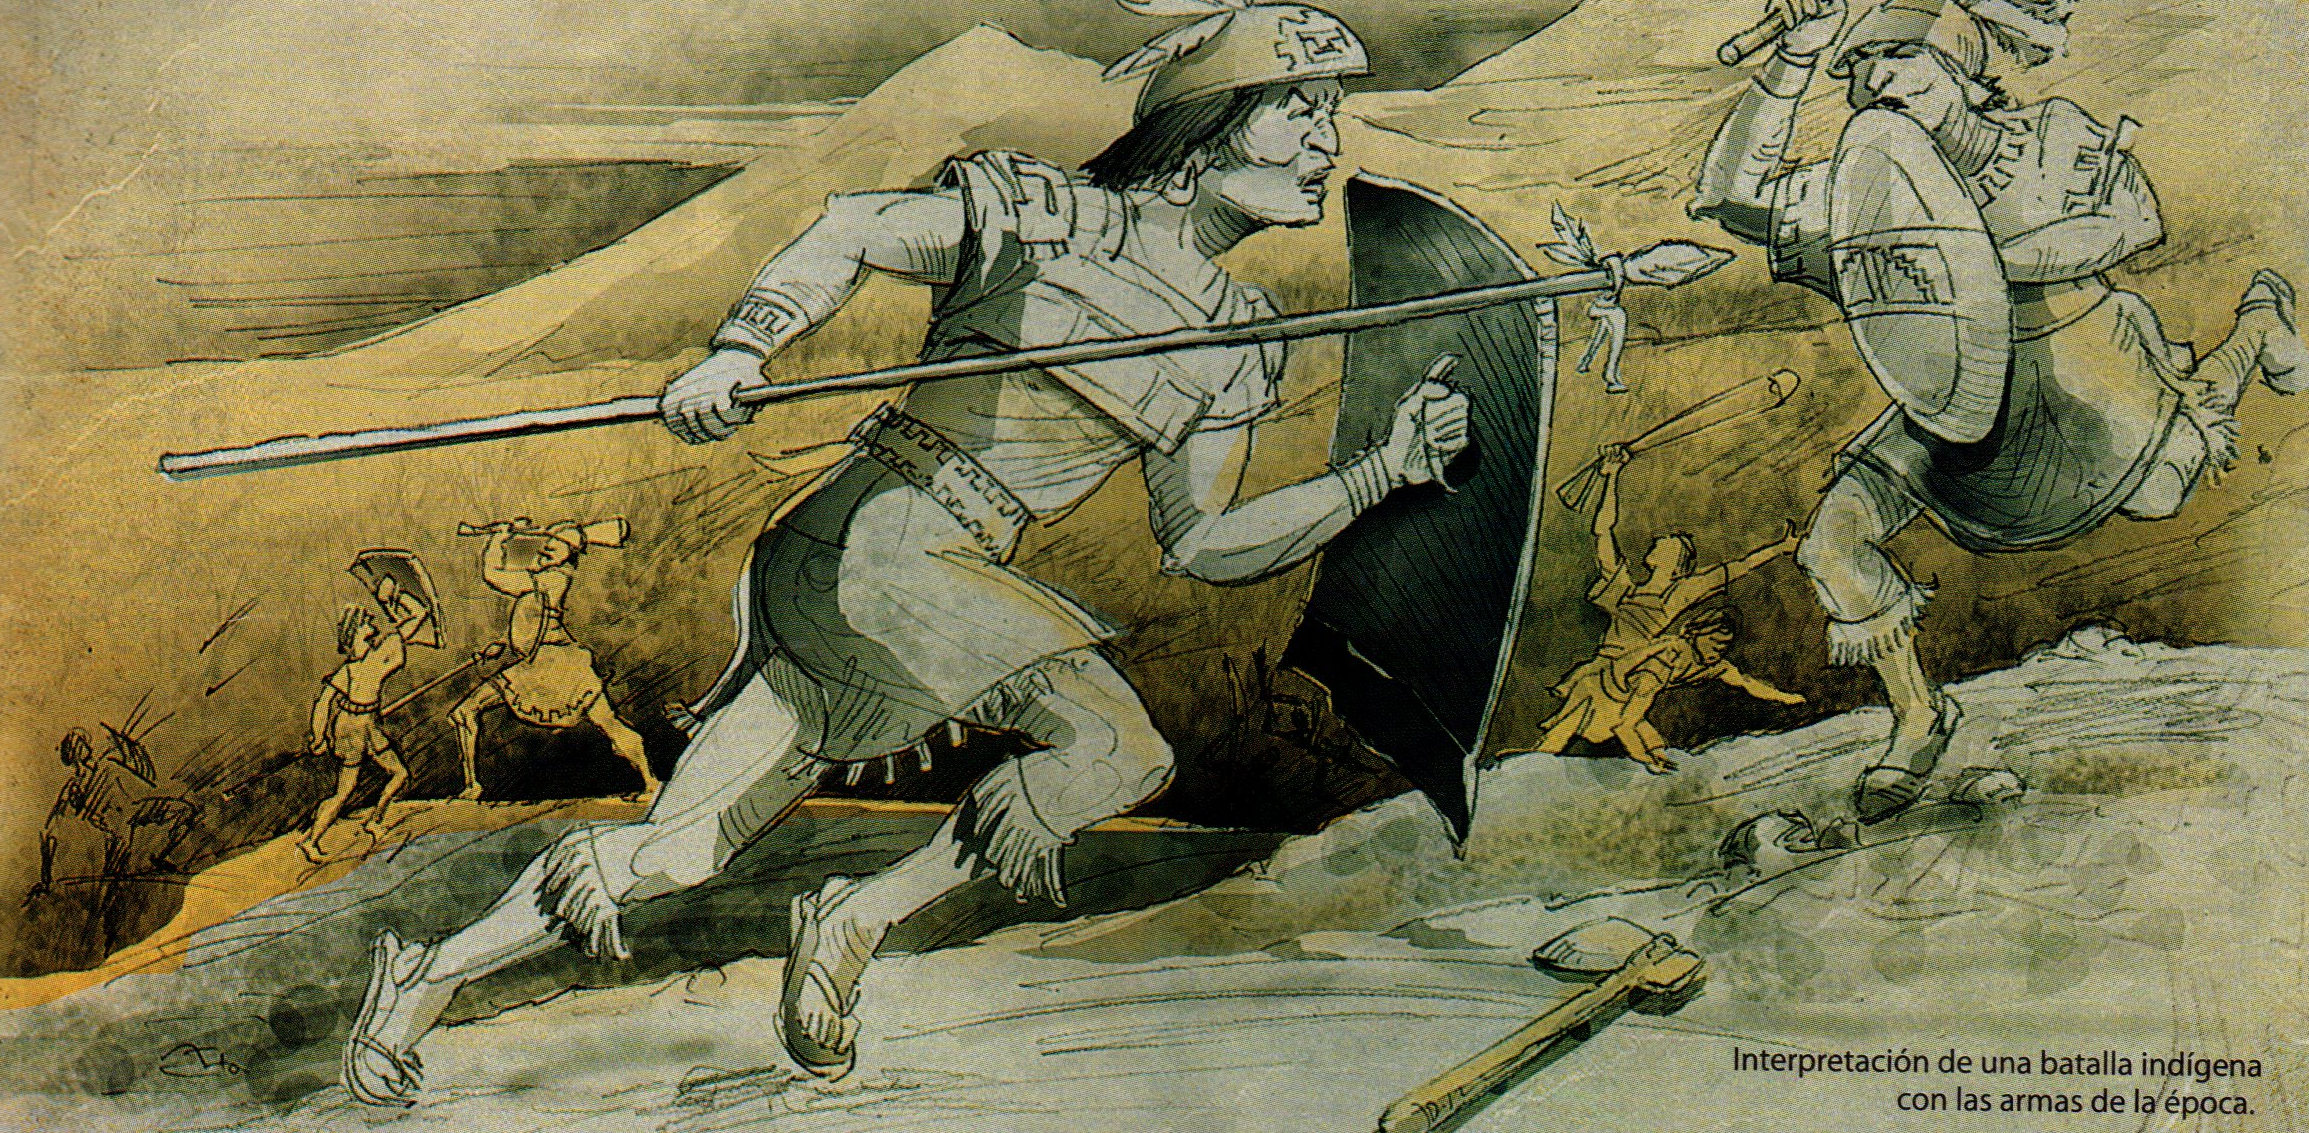
\includegraphics[scale=0.7]{h9}
\centering
\caption{Batalla de Molleambato}
Elaborado por: Carlos Acuña
\label{fig:h9}
\end{figure}
\clearpage
\subsection*{Batalla de Quipaipán}
\justify
\textbf{Antecedentes.} Después de su victoria en Molleambato, Atahualpa se dirigió a Tomebamba, donde fue capturado pero al poco tiempo logró escapar. No tardó en reunir a su ejército y derrotar a los contingentes de Huáscar.\\
Castigó duramente a los habitantes de Tomebamba que lo habían traicionado y se dirigió hacia los huancavilcas para obtener refuerzos. Tras varias varias batallas tomó ciudades como Cusubamba, Collahuayla, Pombo y Yanamarca y continúo su imparable su avance hacia el sur. Huáscar, contrariado por las derrotas, se movilizó con su ejército hasta Quipaipán, muy cerca de Cuzco para defender la capital.\cite{2010batallas} \\ 
\textbf{El enfrentamiento.} Quisquis y Calicuchima se asentaron con su ejército cerca del río Cotabamba y enviaron un contingente para armar un ataque. Mientras que Topa Atao, comandante cuzqueño, se movilizó hacia esa zona para abrirle paso a Huáscar.\\
Calicuchima, por el sur cruzó el río con cinco mil hombres al enterarse que Huáscar descendería por esa zona. Los guerreros del Cuzco recibieron el ataque sin poder defenderse, entonces Calicuchima comunicó a Quisquís que Huáscar seguramente pretendía huir por el norte y lo movilizó hasta allá.\\
Huáscar llegó desprevenido y al ver muertos a sus hombres intentó huir. Quisquís llegó desde el norte, interceptando al emperador cuzqueño y lo capturó. \cite{2010batallas}

\begin{figure}[h]
\captionsetup{justification=centering,margin=2cm}
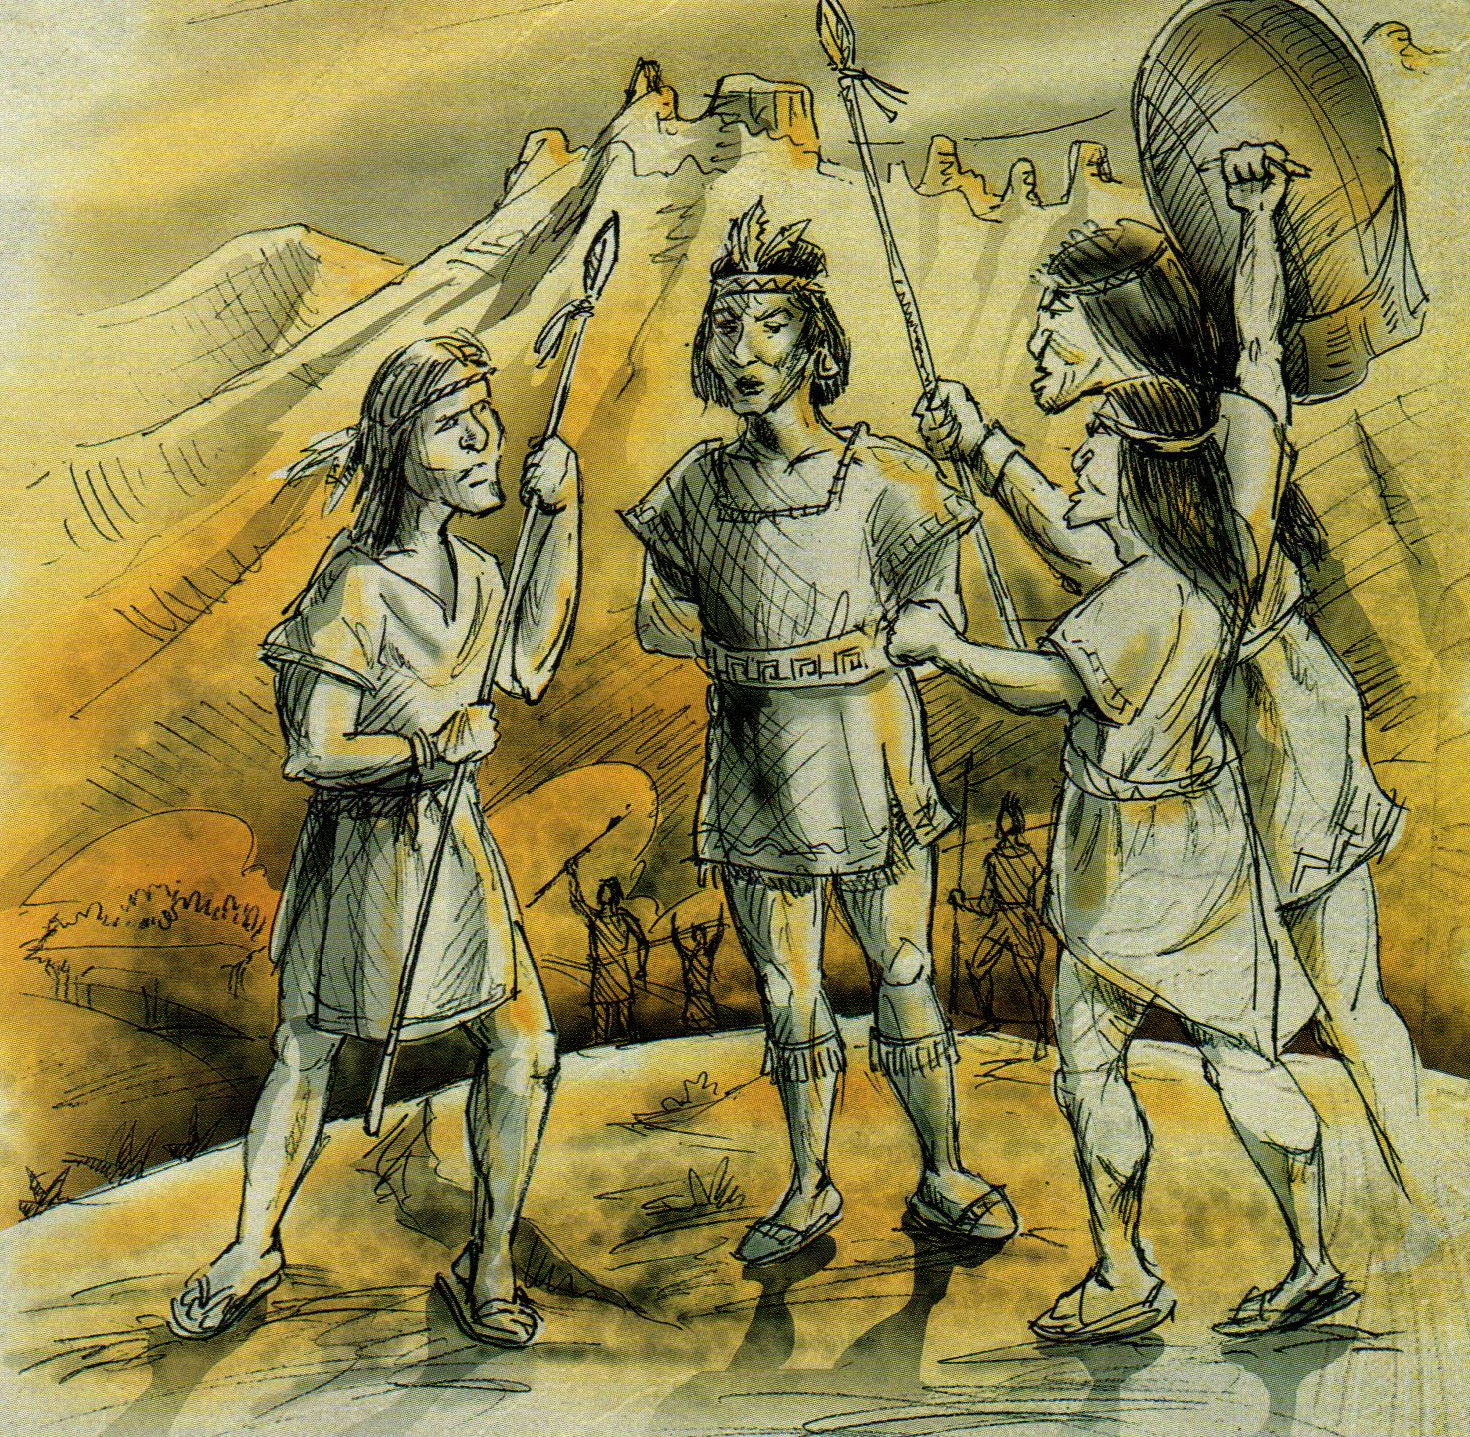
\includegraphics[scale=0.7]{h10}
\centering
\caption{Batalla de Quipaipán}
Elaborado por: Carlos Acuña
\label{fig:h10}
\end{figure}

\clearpage
\subsection*{Mitología inca}
\justify
La mitología inca fue transmitida a través de los siglos mediante un lenguaje oral, ya que este pueblo no contaba con un lenguaje escrito, sin embargo sus dioses y su mitología sobrevivió el paso del tiempo y por lo tanto se conoce lo siguiente.

\subsection*{Bestias mitológicas}
\subsection*{Amaru}
\justify
Es una criatura fusión de animales, ya que tiene forma de serpiente, cabeza de camélido, alas de paraje, garras de león y cola de pez. Está relacionada con el agua, pues esta representa la vida que se encuentra en el elemento acuático, esta criatura se encarga de resguardar la vida que se encuentra en los ríos y lagos. \cite{morel1987diccionario} 

\begin{figure}[h]
\captionsetup{justification=centering,margin=2cm}
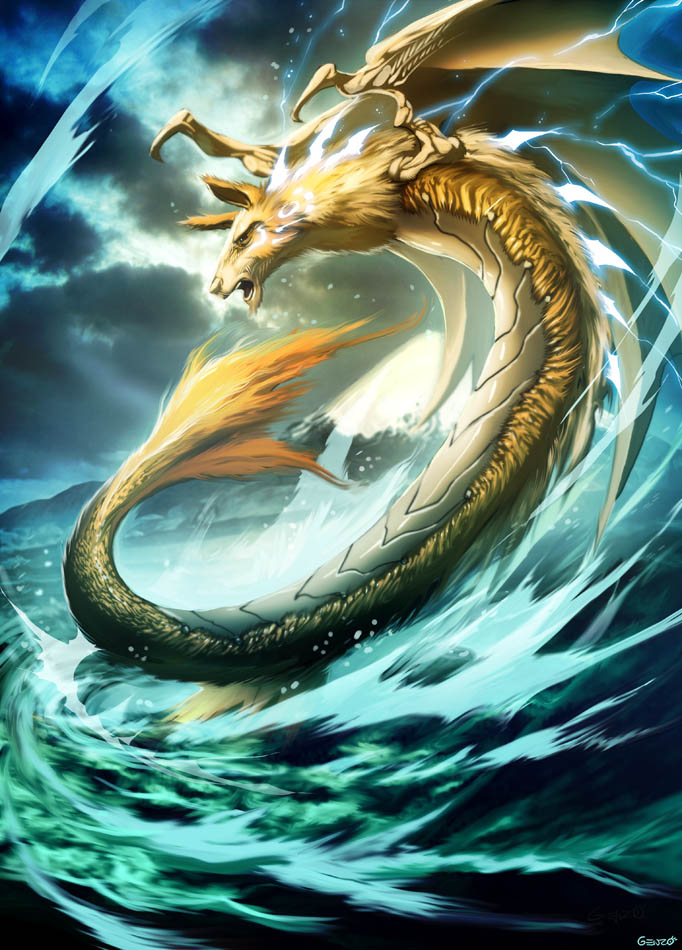
\includegraphics[scale=0.3]{h11}
\centering
\caption{Amaru}
Elaborado por: Carlos Acuña
\label{fig:h11}
\end{figure}

\subsection*{Apallimay}
\justify
Criatura que suele manifestarse en caminos apartados como un inofensivo bebe, el cual pide con llantos que lo carguen, cuanto esto sucede y logra acomodarse en la espalda de su víctima, la criatura comienza a crecer rápidamente hasta convertirse en una pesada carga, con rostro de anciano, una boca con colmillos y fracciones llenas de ira y rencor.\\
Se dice que para que la victima se libere de esta terrible criatura, necesita únicamente los servicios de un curandero, ya que sino el Apallimay tomará la energía vital de la persona hasta provocarle la muerte.\cite{morel1987diccionario} 

\begin{figure}[h]
\captionsetup{justification=centering,margin=2cm}
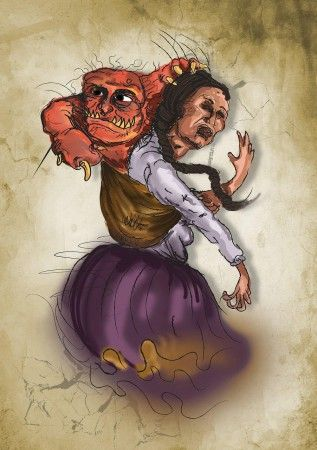
\includegraphics[scale=0.5]{h12}
\centering
\caption{Apallimay}
Elaborado por: Carlos Acuña
\label{fig:h12}
\end{figure}

\subsection*{Jarjacha}
\justify
Según la mitología Inca, cuando una persona comete incesto o infidelidad, su alma puede escapar de su cuerpo y tomar diferentes formas aterradoras. No necesariamente la persona debe estar muerta para que esto pueda suceder, sino que simplemente puede estar dormida.\\
Estas almas suelen representarse como una llama con una o varias cabezas, e incluso puede aparecer con el cuerpo de llama, pero con cabeza de humano, dependiendo de la frecuencia con que cometieron la falta.\\
Según las historias, es muy peligroso encontrarse con estas criaturas, ya que tienen el poder de hipnotizar a las personas mirándolas fijamente a los ojos para luego asesinarlas.\cite{morel1987diccionario}

\begin{figure}[h]
\captionsetup{justification=centering,margin=2cm}
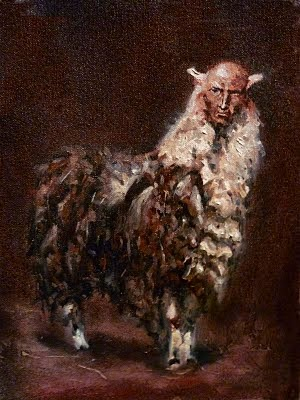
\includegraphics[scale=0.4]{h13}
\centering
\caption{Jarjacha}
Elaborado por: Carlos Acuña
\label{fig:h13}
\end{figure}

\clearpage
\subsection*{Distribución de personajes históricos y mitológicos para el desarrollo del videojuego}

\begin{longtable}{| p{4cm} | p{6cm} |}
\hline
\captionsetup{justification=centering,margin=2cm}
%%Titulo
\textbf{Personaje} & \textbf{Uso}\\ \hline
%%Contenido
Huáscar & Jefe de nivel \\ \hline
Chapera & Jefe de nivel \\ \hline
Apu Atoc & Jefe de nivel \\ \hline
Amaru & Enemigo de nivel \\ \hline
Apallimay & Enemigo de nivel \\ \hline
Jarjacha & Enemigo de nivel \\ \hline
\caption{Personajes del videojuego}
\label{t:elementosJuego}
\end{longtable}
\begin{center}
Elaborado por: Carlos Acuña
\end{center}
%%%%%%%%%%%%%%%%%%%%%%%%%%%%%%%%%CAPITULO 3%%%%%%%%%%%%%%%%%%%%%%%%%%%%%%%%%%%%%%
\chapter{Resultados y Discusión}
\section{Análisis y discusión de los resultados}
\subsection{Estudio de Frameworks para el desarrollo del proyecto}\label{sec:estudioF}
\subsection*{Frameworks}
\justify
En arquitectura de software se usa la palabra framework para describir un conjunto de diseños reusables y código que puede asistir en el desarrollo de software de aplicaciones.
Un framework de aplicaciones provee a los desarrollares una estructura y plantilla que pueden usar como base para construir sus aplicaciones.\\
Los frameworks incluyen clases abstractas, clases concretas e interacciones predefinidas sobre las clases. Siendo así que los desarrolladores pueden reducen el esfuerzo de desarrollo a través de la reutilización de código y diseños proporcionados por el framework \cite{chen2004developing}.  

\subsection*{Unity3D}
\justify
Unity es un framework y motor de videojuegos multiplataforma creado por Unity Technologies. Unity está disponible como plataforma de desarrollo para Microsoft Windows, Mac OS, Linux y dispositivos móviles que permite la creación de videojuegos mediante la utilización de objetos que pueden ser importados hacia la herramienta, como son modelos 2D y 3D, archivos de texto, imágenes, sonidos, etc. Todo es hecho mediante varios lenguajes de programación como son BOO, C\# y Javascript. MonoDevelop es el IDE con el que trabaja Unity además de usar API's para el uso de rutinas, estructura de datos y clases, estas API's también son conocidas como librerías \cite{okita2014learning}.\\
Unity es completamente libre para cualquiera o cualquier empresa que gane menos de \$ 100000 al año, puede ser descargado sin ningún cargo adicional y sin tarjeta de crédito \cite{murray2014c}.

\subsection*{Godot Engine}
\justify
Godot Engine es un software diseñado para crear juegos. Contiene muchas herramientas para crear toda clase de juegos 2D, con varios niveles de complejidad. Tiene un tamaño menor en comparación con otros motores de videojuegos. Godot está disponible bajo licencia MIT, por lo tanto se puede usar de manera libre y redistribuir el juego de cualquier manera.\\
Godot soporta múltiples plataformas y los videojuegos son codificados en C++, C\#. Godot tiene un editor con auto indentación, resaltado
de sintaxis, autocompletado de código y depurador que soporta breakpoints y ejecución paso a paso \cite{manzur2018godot}.

\subsection*{Unreal Engine}
\justify
Unreal Engine fue creado en 1998 con el advenimiento del primer juego de disparos en primera persona Unreal. Esta herramienta soporta DirectX and OpenGL, además de ser viable para otras plataformas como OS X, iOS, Android, Flash, JavaScript y HTML 5, Unreal Engine 4 es la última versión de este motor de videojuegos el cual está completamente programado en C++. \cite{sanders2016introduction}.\\
Unreal Engine utiliza el sistema de secuencias de comandos visuales Bluesprints donde el concepto es utilizar una interfaz basado en nodos para crear elementos de juego desde Unreal Editor. Al igual que muchos lenguajes, se utiliza para definir clases u objetos orientados a objetos en el motor. Este sistema es extremadamente flexible y potente, ya que brinda a los diseñadores la capacidad de utilizar las mismas herramientas que utilizan los programadores.  
\cite{unreal2020}

\subsection{Comparación de diferentes motores de juegos para la creación de la aplicación}
\justify
En la sección \ref{sec:estudioF} se da a conocer algunos de los frameworks de videojuegos que se pueden utilizar para la creación del proyecto. Por lo tanto el cuadro \ref{t:comparacionF} muestra una comparación entre estas herramientas con el fin de escoger la mejor para el desarrollo del proyecto basado en los siguientes criterios.

\begin{itemize}
\item \textbf{Requisitos mínimos.} Se refiere a requisitos tanto de software o hardware que un desarrollador debe disponer.

\item \textbf{Orientación 2D.} Se refiere a la característica del framework que permite realizar videojuegos en 2 dimensiones.

\item \textbf{Licenciamiento.} Se refiere a las licencias que se otorgan a los desarrolladores, tanto gratuitas como pagadas.

\item \textbf{Lenguaje de alto nivel.} Se refiere al lenguaje de programación que el desarrollador debe utilizar para trabajar con el framework de creación de videojuegos.

\item \textbf{Soporte de plataformas.} Se refiere a la posibilidad de correr el juego en varias plataformas.

\item \textbf{Documentación.} Se refiere a la cantidad de documentación disponible de la herramienta que se desea utilizar junto con la ayuda creada por la comunidad que trabaja con el framework.
\end{itemize}
\clearpage

\begin{longtable}{| p{3cm} | p{3cm} | p{3cm} | p{3cm} |}
\hline
\captionsetup{justification=centering,margin=2cm}
%%Titulo
\textbf{} & \textbf{Unity} & \textbf{Godot Engine} & \textbf{Unreal Engine} \\ \hline
%%Contenido
Requisitos mínimos & Windows 7 y Windows 10 64-bit 
& Windows 7 
& Windows 10 64-bit
 \\ \hline
Orientación 2D & 2D
& 2D
& 2D
 \\ \hline
Licenciamiento & Completamente libre para cualquiera o cualquier empresa que gane menos de \$ 100000 al año
 & MIT License 
 & 5\% de regalías cuando las ventas del juego superan los \$ 3000
 \\ \hline
Lenguaje de alto nivel & C\#, Javascript
 & GDScript
 & C++
 \\ \hline
Soporte de plataformas & Windows, Mac, Linux
 & Windows, Mac, Linux  
 & Windows, Mac, Linux
 \\ \hline
Documentación & Existe documentación tanto en la página oficial de Unity como en foros, videos, blogs y varios sitios de Internet 
 & Existe documentación en la página oficial de Godot pero muy poca información en otros recursos externos
 & Existe documentación en la página oficial de Unreal Engine pero es demasiado básica y en otros recursos la mayoría de la ayuda conlleva el pago de una cantidad de dinero\\ \hline

\caption{Cuadro comparativo de motores de juegos}
\label{t:comparacionF}
\end{longtable}
\begin{center}
Elaborado por: Carlos Acuña
\end{center}

\justify
En base a los resultados obtenidos se puede determinar que Unity tiene más ventaja sobre los otros dos motores de juego, especialmente en el apartado de documentación ya que al existir una gran cantidad de información hace que la herramienta sea más fácil de entender y se pueda consultar sobre cualquier problema en el transcurso del proyecto.

\subsection{Componentes de la interfaz de Unity}

\subsection*{Interfaz de Unity}
Unity está conformado por ventanas que muestran varias partes del proyecto que se está ejecutando, las cuales se puede reorganizar, agrupar, separar y acoplar como se muestra en la figura \ref{fig:unity01}

\begin{figure}[h]
\captionsetup{justification=centering,margin=2cm}
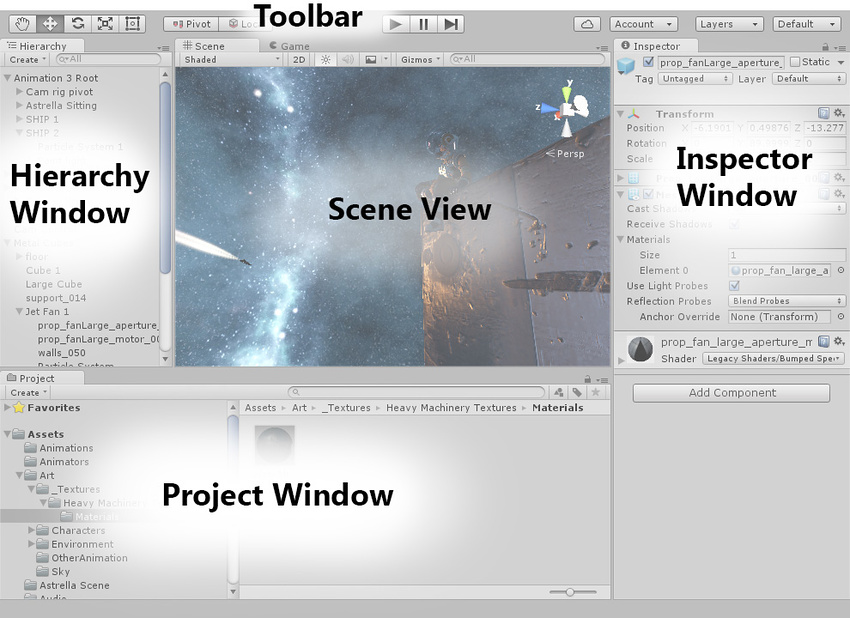
\includegraphics[scale=0.4]{unity01}
\centering
\caption{Editor de Unity}
Elaborado por: Carlos Acuña
\label{fig:unity01}
\end{figure}
\clearpage
\begin{itemize}

\item \textbf{Project Window.} (ventana del proyecto) muestra los assets de librería que están disponibles para ser usados. Cuando se importe los assets al proyecto, estos aparecen aquí \cite{2020unity}.

\begin{figure}[h]
\captionsetup{justification=centering,margin=2cm}
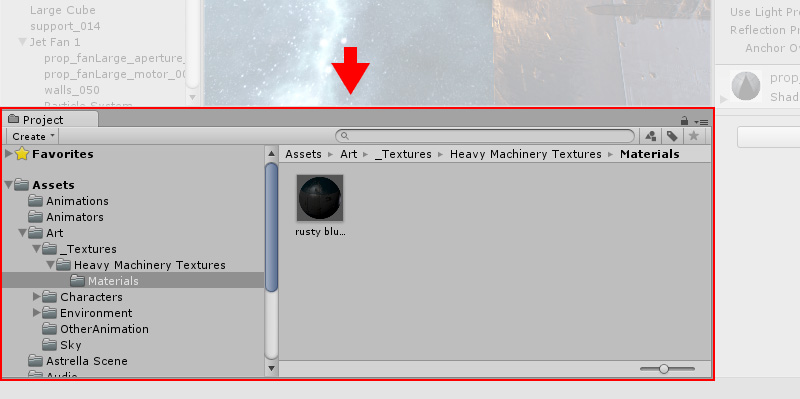
\includegraphics[scale=0.4]{unity02}
\centering
\caption{Project Window de Unity}
Elaborado por: Carlos Acuña
\label{fig:unity02}
\end{figure}

\item \textbf{ Scene View.} (vista de escena) permite la navegación visual y editar la escena. La scene view puede mostrar una perspectiva 2D o 3D dependiendo en el tipo de proyecto en el que la que se está trabajando \cite{2020unity}.

\begin{figure}[h]
\captionsetup{justification=centering,margin=2cm}
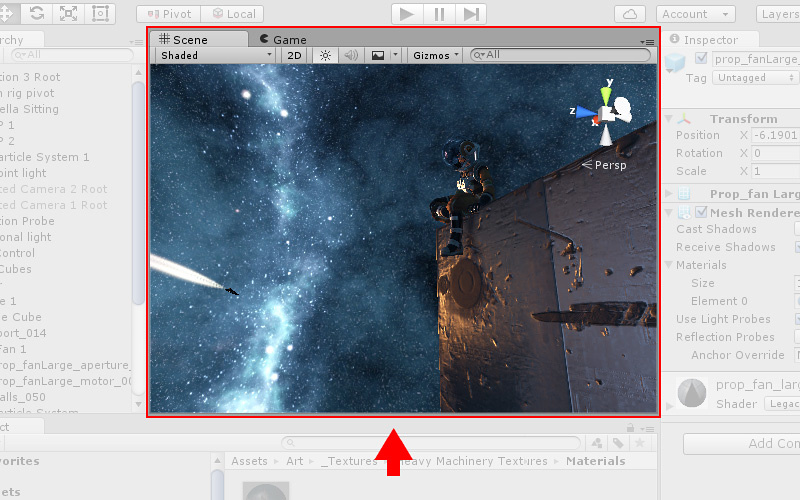
\includegraphics[scale=0.4]{unity03}
\centering
\caption{Scene View de Unity}
Elaborado por: Carlos Acuña
\label{fig:unity03}
\end{figure}
\clearpage
\item \textbf{ Hierarchy Window.} (vista de jerarquía) es una representación de texto jerárquico de cada objeto en la escena. Cada elemento en la escena tiene una entrada en la jerarquía, por lo que las dos ventanas están inherentemente vinculadas. La jerarquía revela la estructura de cómo los objetos están agrupados el uno al otro \cite{2020unity}.

\begin{figure}[h]
\captionsetup{justification=centering,margin=2cm}
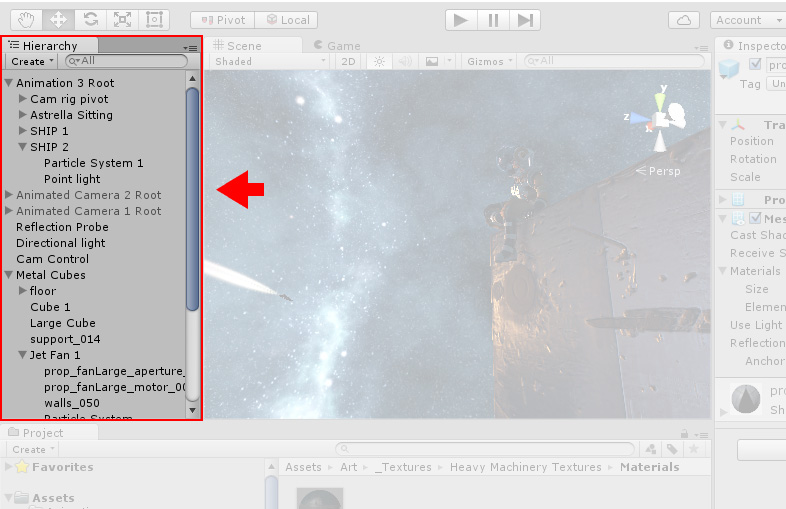
\includegraphics[scale=0.4]{unity04}
\centering
\caption{Hierarchy Window de Unity}
Elaborado por: Carlos Acuña
\label{fig:unity04}
\end{figure}

\item \textbf{ Inspector Window.} (ventana de inspector) permite visualizar y editar todas las propiedades del objeto actualmente seleccionado. Ya que diferentes objetos tienen diferentes propiedades, el layout (diseño) y contenido de la ventana del inspector va a variar \cite{2020unity}.

\begin{figure}[h]
\captionsetup{justification=centering,margin=2cm}
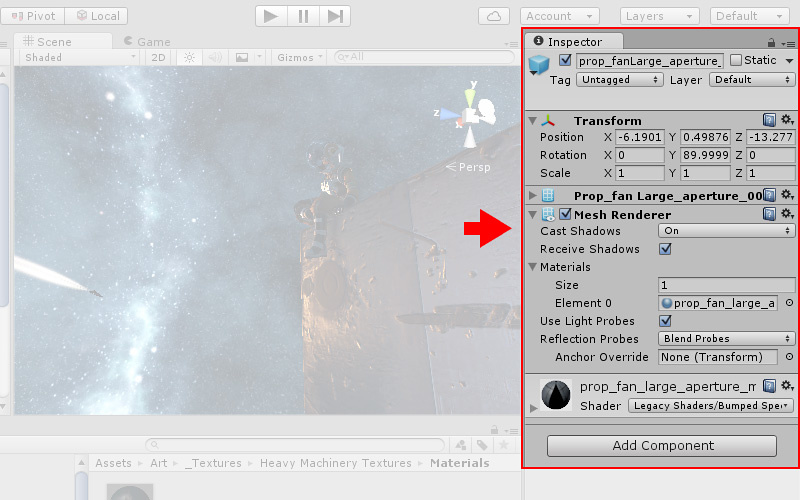
\includegraphics[scale=0.4]{unity05}
\centering
\caption{Inspector Window de Unity}
Elaborado por: Carlos Acuña
\label{fig:unity05}
\end{figure}
\clearpage
\item \textbf{ Toolbar.} (barra de herramientas) proporciona un acceso a las características más esenciales para trabajar. En la izquierda contiene las herramientas básicas para manipular la scene view y los objetos dentro de esta. En el centro están los controles de reproducción, pausa, y pasos. Los botones a la derecha le dan acceso a sus servicios de Unity Cloud y su cuenta de Unity, seguido por un menú de visibilidad de capas, y finalmente el menú del layout del editor (que proporciona algunos diseños alternativos para la ventana del editor, y permite guardar layouts personalizados). La barra de herramienta no es una ventana, y solamente es parte de la interfaz de Unity que usted no puede re-ajustar \cite{2020unity}.

\begin{figure}[h]
\captionsetup{justification=centering,margin=2cm}
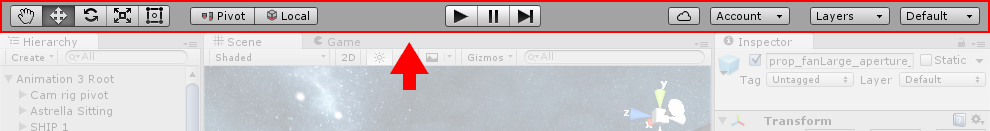
\includegraphics[scale=0.4]{unity06}
\centering
\caption{Toolbar de Unity}
Elaborado por: Carlos Acuña
\label{fig:unity06}
\end{figure}
\end{itemize}

\subsection*{GameObject}
\justify
Los GameObjects son objetos fundamentales en Unity que representan personajes, props, y el escenario. Estos no logran nada por sí mismos pero funcionan como contenedoras para Components, que implementan la verdadera funcionalidad.\\
Un GameObject siempre tiene el componente Transform adjunto (para representar la posición y orientación) y no es posible quitar esto. Los otros componentes que le dan al objeto su funcionalidad pueden ser agregados del menú Component del editor o desde un script. También hay muchos objetos útiles pre-construidos (figuras primitivas, cámaras, etc) \cite{2020unity}.

\begin{figure}[h]
\captionsetup{justification=centering,margin=2cm}
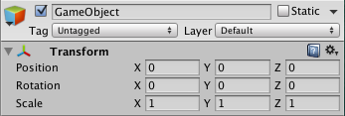
\includegraphics[scale=1]{unity07}
\centering
\caption{GameObject de Unity}
Elaborado por: Carlos Acuña
\label{fig:unity07}
\end{figure}

\subsection*{Transform Component}
\justify
Es imposible crear un GameObject en el Editor sin un Transform Component. Este componente define la posición del GameObject, la rotación y la escala en el mundo del juego y Scene view. El Transform Component también habilita un concepto llamado ‘crianza de los hijos’, que es una parte crítica del trabajo con GameObjects \cite{2020unity}. 
\clearpage
\subsection*{Prefabs}
\justify
En el sistema prefabricado de Unity, los Prefabs actúan como plantillas. Se crean Prefabs en el editor y se guardan como un activo en la ventana del proyecto. Desde Prefabs, se puede crear cualquier número de instancias prefabricadas. Las instancias prefabricadas pueden crearse en el editor y guardarse como parte de sus escenas, o instanciarse en tiempo de ejecución \cite{2020unity}.

\begin{figure}[h]
\captionsetup{justification=centering,margin=2cm}
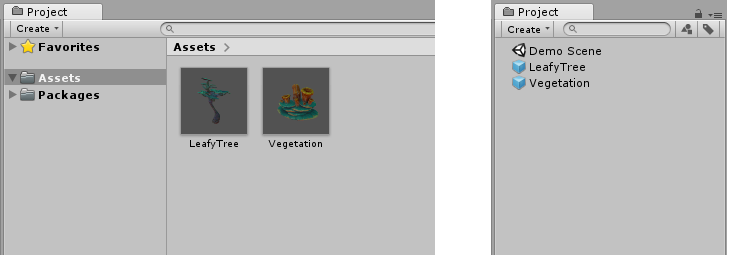
\includegraphics[scale=0.4]{unity08}
\centering
\caption{Prefabs de Unity}
Elaborado por: Carlos Acuña
\label{fig:unity08}
\end{figure}

\subsection*{Input Convencional de Juego}
\justify
Unity soporta teclado, joystick y gamepad input.\\
Se pueden crear ejes y botones virtuales en la ventana de entrada, y los usuarios finales pueden configurar la entrada del teclado en un bonito diálogo de configuración de pantalla \cite{2020unity}.

\begin{figure}[h]
\captionsetup{justification=centering,margin=2cm}
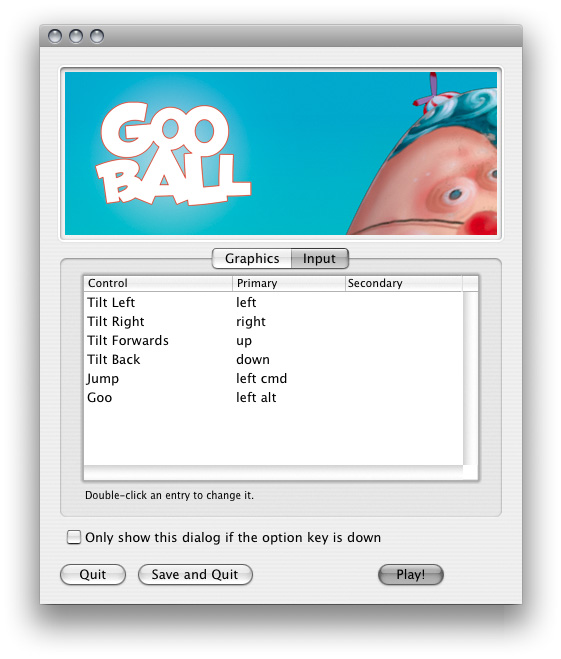
\includegraphics[scale=0.4]{unity09}
\centering
\caption{Input de Unity}
Elaborado por: Carlos Acuña
\label{fig:unity09}
\end{figure}

\subsection*{Virtual Axes (Ejes Virtuales)}
\justify
Desde los scripts, todos los ejes virtuales son accedidos por su nombre.
Cada proyecto tiene el siguiente eje input por defecto cuando es creado:\\
Horizontal y Vertical son asignados a las teclas w, a, s, d y las teclas de flecha.\\
Fire1, Fire2, Fire3 están asignadas a las teclas Control, Option (Alt), y Command, respectivamente.\\
Mouse X y Mouse Y están asignados al movimiento delta del mouse.\\
Window Shake X y Window Shake Y es asignado al movimiento de la ventana.\\

\begin{figure}[h]
\captionsetup{justification=centering,margin=2cm}
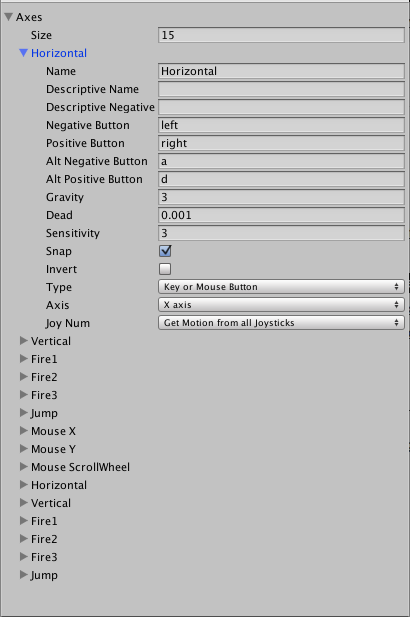
\includegraphics[scale=0.5]{unity10}
\centering
\caption{Virtual Axes de Unity}
Elaborado por: Carlos Acuña
\label{fig:unity10}
\end{figure}

\clearpage
\subsection{Selección de metodologías ágiles para el desarrollo de videojuegos}\label{sec:estudioM}
\justify
Al desarrollar un proyecto de software es prudente utilizar un metodología de desarrollo, preferiblemente ágil, con el fin de desarrollar un proyecto de manera ordenada, que tenga que cumplir metas en un tiempo determinado y que no se desperdicie recursos valiosos durante la creación del software.
\subsection*{Metodologías}
\subsection*{SUM}
\justify
La metodología SUM para videojuegos tiene como objetivo desarrollar videojuegos de calidad en tiempo y costo, así como la mejora continua del proceso para incrementar su eficacia y eficiencia. Pretende obtener resultados predecibles, administrar eficientemente los recursos y riesgos del proyecto, y lograr una alta productividad del equipo de desarrollo. SUM fue concebida para que se adapte a equipos multidisciplinarios pequeños (de tres a siete integrantes que trabajan en un mismo lugar físico o estén distribuidos), y para proyectos cortos (menores a un año de duración) con alto grado de participación del cliente.\cite{Acerenza2009}\\
\subsection*{Roles}
\justify
La metodología define cuatro roles: equipo de desarrollo, productor interno, cliente y verificador beta. El productor interno y el cliente se relacionan en forma directa con los roles de SCRUM Master y Product Owner de SCRUM respectivamente.\\
\begin{itemize}
\item \textbf{Equipo de desarrollo}. Tiene las características del Scrum team, pero a
diferencia de SCRUM se definen subroles dentro del equipo, estos son equivalentes
a los usados por la industria local tales como: programador, artista gráfico,
artista sonoro y diseñador de juego. Es necesario esta definición ya que se requiere una alta especialización para satisfacer las distintas disciplinas que involucra del desarrollo de videojuegos, aspecto no contemplado en Scrum \cite{Acerenza2009}. El equipo de desarrollo consta de:
\begin{itemize}
\item \textbf{Programador.} Define la arquitectura, realiza el dise˜no, implementación y verificación de los componentes de software e integra el contenido audiovisual del videojuego. \cite{Acerenza2009}
\item \textbf{Artista gráfico.} Realiza el
arte de concepto, el arte 2D, el modelado 3D y la creación de animaciones y
texturas. \cite{Acerenza2009}
\item \textbf{Artista sonoro.} Se encarga de la creación, grabación, mezcla y edición de los efectos de sonido y música del juego. \cite{Acerenza2009}
\item \textbf{Diseñador de juego.} Es el encargado de diseñar el gameplay, la historia, el ambiente, los personajes y todos los elementos que hacen a la experiencia del jugador. Además, diseña los niveles, misiones y los desafíos que enfrenta el jugador. \cite{Acerenza2009}
\end{itemize}
\item \textbf{Productor interno.} Responsable de la planificación y ejecución del proyecto, define los objetivos y ayuda a resolver problemas que ocurren en el proyecto. Se comunica con el cliente y mantiene al equipo de desarrollo enfocado en el proyecto. \cite{Acerenza2009}
\item \textbf{Cliente.} Es el dueño del producto que valida el concepto del juego, aprueba los planes del juego, prioriza las tareas del videojuego y participa en la evaluación del proyecto. \cite{Acerenza2009} 
\item \textbf{Verificador Beta}. Realizan la verificación funcional del videojuego. Dependiendo del tamaño del proyecto pueden participar varios verificadores beta \cite{Acerenza2009} 
\end{itemize}
\subsection*{Ciclo de vida}
\justify
El ciclo de vida se divide en fases iterativas e incrementales que se ejecutan en
forma secuencial con excepción de la fase de gestión de riesgos que se realiza durante todo el proyecto. Las cinco fases secuenciales son: concepto, planificación, elaboración, beta y cierre. \cite{Acerenza2009} 
\begin{itemize}
\item \textbf{Concepto.} Tiene como objetivo principal definir el concepto del videojuego lo que implica definir aspectos de negocio (público objetivo, modelo de negocio), de elementos de juego (principales características, gameplay, personajes e historia entre otros) y técnicos (lenguajes y herramientas para el
desarrollo). El concepto del videojuego se construye a partir de ideas y propuestas de cada rol involucrado sobre los aspectos a definir. Las propuestas
se refinan a través de reuniones y se analiza su factibilidad con pruebas de
concepto. Esta fase analiza cuando se tiene el concepto validado entre todas
las partes involucradas. \cite{Acerenza2009}
\item \textbf{Planificación.} La fase tiene como objetivo principal planificar las restantes fases del proyecto. Para ello es necesario definir el cronograma del proyecto junto con sus principales hitos, conformar el equipo para la fase de elaboración de acuerdo a las necesidades técnicas del proyecto, determinar y
tercerizar las tareas que el equipo no pueda cumplir, definir el presupuesto
y especificar el videojuego. \cite{Acerenza2009}
\item \textbf{Elaboración.} El objetivo de esta fase es implementar el videojuego. Para ello se trabaja en forma iterativa e incremental para lograr una versión ejecutable del videojuego al analizar cada iteración. \cite{Acerenza2009}
\item \textbf{Beta.} La fase tiene como objetivos evaluar y ajustar distintos aspectos del videojuego como por ejemplo gameplay, diversión, curva de aprendizaje y curva de dificultad, además de eliminar la mayor cantidad de errores detectados. Se trabaja en forma iterativa liberando distintas versiones del videojuego para verificar. Para ello primero se distribuye la versión beta del videojuego a verificar y se determinan los aspectos a evaluar y la forma de comunicación. Mientras la versión se verifica, se envían reportes con los errores o evaluaciones realizadas. Estos reportes son analizados para ver la necesidad de
realizar ajustes al videojuego. Se puede optar por liberar una nueva versión
del videojuego para verificar una vez que se realizan los ajustes. El ciclo
termina cuando se alcanza el criterio de finalización establecido en el plan
del proyecto. \cite{Acerenza2009}
\item \textbf{Cierre.} Esta fase tiene como objetivos entregar la versión final del videojuego al cliente según las formas establecidas y evaluar el desarrollo del proyecto. Para la evaluación se estudian los problemas ocurridos, los éxitos conseguidos, las soluciones halladas, el cumplimiento de objetivos y la certeza de las estimaciones. Con las conclusiones extraídas se registran las lecciones
aprendidas y se plantean mejoras a la metodología. En la evaluación es recomendable que participen todas las personas que han estado involucradas
en el proyecto. \cite{Acerenza2009}
\item \textbf{Gestión de riesgos.} Esta fase se realiza durante todo el proyecto con el objetivo de minimizar la ocurrencia y el impacto de problemas. Esto se debe a que distintos riesgos pueden ocurrir en cualquiera de las fases, por lo cual siempre debe existir un seguimiento de los mismos. Para cada uno de los
riesgos que se identifican se debe establecer la probabilidad y el impacto
de ocurrencia, mecanismos de monitoreo, estrategia de mitigación y plan de
contingencia. \cite{Acerenza2009}
\end{itemize} 

\subsection*{DAV}
\justify
DAV (Desarrollo Ágil de Videojuegos), es una metodología que nace con la unión
de las características de SCRUM y XGD, con la finalidad de proporcionar una
estructura que permita la creación de videojuegos de forma técnica y sencilla.
Esta metodología se compone de los siguientes elementos: valores, prácticas, roles, reuniones, fases, artefactos y herramientas. \cite{Implementacion2011}

\subsection*{Prácticas}
\justify
DAV utiliza prácticas tanto de SCRUM como de XGD.
\begin{itemize}
\item \textbf{Equipo completo.} El Equipo DAV debe permanecer en comunicación coherente, ser un todo.\cite{Implementacion2011}
\item \textbf{Diseño incremental.} Las tareas de un videojuego deben ser de la forma más sencilla posible, que funcionen correctamente.\cite{Implementacion2011}
\item \textbf{Historias de usuario.} Se trata de una breve descripción de las funcionalidades del videojuego, por lo general descrito por el Dueño del Producto.\cite{Implementacion2011} 
\item \textbf{Ciclos semanales.} El proyecto está organizado y planificado para ser ejecutado en ciclos de corta duración.\cite{Implementacion2011}
\item \textbf{Integración continua.} En el proyecto existirán trozos de código fuente que continuamente se integrarán en funcionamiento.\cite{Implementacion2011}
\item \textbf{Código compartido.} Todo el Equipo DAV compartirá el código fuente del proyecto. \cite{Implementacion2011} 
\item \textbf{Reuniones diarias de seguimiento.} Reuniones rápidas del proyecto, con el objetivo de que todo el Equipo DAV esté consciente de la labor que se está realizando en un momento dado. En la mayoría de estas reuniones, gran parte de los participantes simplemente escuchan, sin tener mucho que aportar. \cite{Implementacion2011} 
\item \textbf{Entregas pequeñas.} Producir rápidamente versiones del videojuego que sean jugables, aunque no cuenten con toda la funcionalidad del videojuego. Esta versión ya constituirá un resultado de valor para el negocio. \cite{Implementacion2011} 
\item \textbf{Pruebas.} El videojuego será probado en varios momentos por diferentes personas, dando como resultado una información valiosa que podrá ser tomada como base para decisiones futuras. \cite{Implementacion2011} 
\item \textbf{Refactorización.} Es una actividad constante de reestructuración del código con el objetivo de evitar duplicaciones, mejorar la legibilidad, simplificarlo y hacerlo más flexible para facilitar posteriores cambios. \cite{Implementacion2011}  
\item \textbf{Desarrollo en parejas (Cuando el Equipo Dav sea grande).} Toda la producción del videojuego debe realizarse con trabajo en parejas, pero simplemente los programadores y diseñadores. Esto conlleva ventajas implícitas (menor tasa de errores, mejor diseño y mayor satisfacción del equipo). \cite{Implementacion2011} 
\item \textbf{Contacto directo.} Los clientes se convierten en parte del equipo de desarrollo, de esta manera existe comunicación cara a cara. \cite{Implementacion2011} 
\item \textbf{Planes de riesgo y Mitigación.} Se desarrollan planes de riesgos y mitigación frecuentes por parte del Equipo DAV, la mitigación de riesgos, la monitorización y la gestión de riesgos se lleva a cabo en todas las etapas y con compromiso. \cite{Implementacion2011} 
\item \textbf{Transparencia.} La transparencia en la planificación y desarrollo de módulos, permitirá a cada uno saber quién es responsable de qué y cuándo. \cite{Implementacion2011} 
\item \textbf{Frecuentes reuniones.} Las frecuentes reuniones permite a las personas involucradas en el negocio monitorizar el progreso. \cite{Implementacion2011} 
\item \textbf{Planificación ágil.} La planificación debe ser distribuida a lo largo del proyecto y no se concentrará en una determinada etapa. Las funciones más importantes serán planeadas con más detalle. Se debe evitar la planificación y estimación de las cosas que pueden no ser parte del videojuego. \cite{Implementacion2011} 
\item \textbf{Establecimiento de prioridades.} A lo largo del proyecto se llevan a cabo varias priorizaciones, que permiten al Equipo DAV trabajar siempre en lo que es más importante. \cite{Implementacion2011} 
\item \textbf{Estimación de Póquer.} Es una práctica ágil para reducir las dificultades habituales en las reuniones de trabajo para la planificación por juicio de expertos. En estas reuniones los participantes emplean un juego de cartas para concretar las unidades de esfuerzo que estiman para cada tarea. \cite{Implementacion2011} 
\end{itemize}
\subsection*{Roles}
\justify
Los roles de DAV se basan únicamente en los de la metodología Scrum, además se incluye en el Equipo DAV el rol de Tester, siendo estos necesarios y suficientes para ser aplicados en equipos pequeños. \cite{Implementacion2011} 
\begin{itemize}
\item \textbf{Dueño del producto.} El Dueño del Producto es la única persona autorizada para decidir sobre cuáles funcionalidades y características funcionales tendrá el videojuego. Es quien representa al cliente y todas aquellas partes interesadas en el videojuego, además es quien maneja y prioriza las funcionalidades a desarrollar y las coloca en la Reserva de Producto. \cite{Implementacion2011} 
\item \textbf{DAV Máster.} El DAV Máster no es un líder típico, sino es un auténtico servidor neutral, que será el encargado de enseñar la metodología DAV a cada integrante implicado en el proyecto, preocupándose de poner la metodología en práctica de modo que se encuentre dentro de la cultura de la organización y así entregue las ventajas previstas, asegurándose de que cada uno siga las reglas y prácticas de DAV. \cite{Implementacion2011}
\item \textbf{Equipo DAV.} Es un equipo multidisciplinario y auto-organizado, su función principal es construir el videojuego que el Dueño del Producto especifica. \cite{Implementacion2011}
\begin{itemize}
\item \textbf{Diseñador.} Realiza el diseño conceptual, define las reglas y mecánicas, escribe el guión y diseña los niveles del videojuego. \cite{Implementacion2011}
\item \textbf{Programador.} Implementa la funcionalidad pedida en el diseño, programa la lógica del juego, gráficos, IA y audio y maneja herramientas/motores (infraestructura). \cite{Implementacion2011}
\item \textbf{Artista.} Construye los objetos, personajes, niveles y anima a los personajes. \cite{Implementacion2011}
\item \textbf{Sonidista.} Crea los sonidos, estilos, efectos y ambientes sonoros para el videojuego. \cite{Implementacion2011}
\item \textbf{Tester.} Verifica el contenido y evalúa la jugabilidad. \cite{Implementacion2011}
\end{itemize}
\item \textbf{Interesados (Clientes).} Se refiere a la gente que hace posible el proyecto y para quienes el videojuego producirá el beneficio acordado que justifica su producción. Sólo participan directamente durante las revisiones de Iteración. \cite{Implementacion2011}
\end{itemize}
\subsection*{Fase Pre-juego}
\justify
En esta fase se realiza la concepción de la idea del juego del Dueño del Producto con ayuda de los miembros del Equipo, es decir, los aspectos fundamentales que conformarán el videojuego. \cite{Implementacion2011}
\begin{itemize}
\item \textbf{Género.} Se debe especificar el género o géneros al que pertenece el videojuego para establecer las características básicas que tendrá en su posterior diseño. \cite{Implementacion2011}
\item \textbf{Historia.} Se debe realizar un bosquejo de la trama o historia del videojuego a desarrollar, indicando qué se quiere contar y cómo se quiere contar. \cite{Implementacion2011}
\item \textbf{Bocetos.} Se crean bocetos o diseños preliminares de los personajes y de dónde trascurrirá la acción del videojuego, ya sean decorados, ambientaciones, ropaje, música, movimientos, etc. \cite{Implementacion2011}
\item \textbf{Aspecto.} A partir de los bocetos se define el aspecto gráfico y artístico del videojuego, colores, temas dominantes, musicalidad, técnicas de diseño 3D o 2D, posiciones de cámaras, etc. \cite{Implementacion2011}
\item \textbf{Interfaz de usuario.} Se define la manera de cómo interactuará el jugador con el videojuego y con qué mecanismos contará para ello. \cite{Implementacion2011}
\item \textbf{Objetivos.} Cuáles son las metas del videojuego, de acuerdo a la historia de éste. \cite{Implementacion2011}
\item \textbf{Reglas.} Qué cosas podemos hacer y cómo vamos a dejar que se hagan. \cite{Implementacion2011} 
\item \textbf{Características.} Especificación de las principales características de cada personaje del videojuego y de los elementos que intervienen en éste. \cite{Implementacion2011}  
\item \textbf{Jugabilidad.} Es aquí donde se definirá cómo se va a jugar, de qué manera se va a jugar, qué cosas podemos hacer en el juego y cómo va reaccionar el entorno del juego a las acciones del jugador a través del personaje. A su vez se debe establecer cómo será la curva de aprendizaje del jugador. Todo esto sin entrar en detalles gráficos, sonoros o de historia. \cite{Implementacion2011} 
\item \textbf{Diseño de niveles.} Describir qué niveles, según la historia o dificultad, se tendrá, cómo serán éstos, cuántos serán, y qué dificultad y retos se plantearán en cada uno de ellos. \cite{Implementacion2011} 
\item \textbf{Requerimientos técnicos.} Establecer los requerimientos técnicos de equipo que necesitará el videojuego para poder ejecutarse. \cite{Implementacion2011}
\item \textbf{Marketing.} Parte fundamental, debido a que muchos videojuegos de inversiones millonarias han ido al traste por una mala campaña de publicidad, para evitar esto hay que establecer las líneas de publicidad para el videojuego. \cite{Implementacion2011}
\end{itemize}
\subsection*{Fase Juego}
\justify
En esta fase se tiene bien definido el alcance del proyecto, por lo tanto ya existe una idea clara de lo que realmente es el videojuego y lo que se debe hacer. \cite{Implementacion2011}
\begin{itemize}
\item \textbf{Iteraciones.} Esta fase que suele llamarse Iteración, consta de ciclos que pueden durar de 1 a 4 semanas (por lo general 1-2 semanas), donde se desarrollan las funcionalidades del videojuego, su duración debe ser constante en cada ciclo. Sin embargo, este requisito no es estricto debido a que a veces el tiempo de cada Iteración es diferente. Una iteración cumple los siguientes pasos \cite{Implementacion2011}
\begin{itemize}
\item \textbf{Elaborar.} Se desarrollan las funcionalidades o requisitos del videojuego que se encuentran en la Reserva de Iteración. \cite{Implementacion2011}
\item \textbf{Integrar.} Las funcionalidades desarrolladas son continuamente integradas en la nueva versión del videojuego. \cite{Implementacion2011}
\item \textbf{Revisar.} Se examinan las funcionalidades desarrolladas en la Iteración para corregir posibles errores y probar que su funcionalidad sea correcta. \cite{Implementacion2011}
\item \textbf{Ajustar.} Se adecua las funcionalidades del videojuego desarrolladas encajándolas correctamente, además se realiza la refactorización del código de las mismas. \cite{Implementacion2011}
\end{itemize}
\end{itemize}

\subsection*{Fase post-juego}
\justify
Esta fase comienza cuando el equipo DAV ha desarrollado con éxito todas las Historias de Usuario y el Dueño del Producto ya no tiene más funcionalidades para implementar. Aquí se realiza el cierre del proyecto, donde se prepara la liberación del videojuego, se verifican las versiones a entregar, se genera la documentación final y se realiza el pre-lanzamiento y el lanzamiento. \cite{Implementacion2011}

\subsection*{Artefactos}
\justify
En el caso de los artefactos, se han constituido en base a una selección mayoritaria de los artefactos de Scrum complementados con los de XGD, para mantener organizado el proyecto. Estos artefactos, ayudan a planificar y revisar cada uno de las Iteraciones, aportando medios ineludibles para efectuar cada una de las reuniones, los mismos se detallan a continuación \cite{Implementacion2011}:
\begin{itemize}
\item \textbf{Historia de usuario.}
Es la definición de un requisito (normalmente una funcionalidad) que el Dueño del Producto quiere, con total claridad y sin ninguna ambigüedad, la cual el Equipo DAV deberá desarrollar como parte de una Iteración.
Son el resultado de escuchar al Dueño del Producto y ayudarle a resumir el requisito en una sola frase. Algo muy importante es que están escritas con el vocabulario del cliente, no con vocabulario técnico. \cite{Implementacion2011}

\begin{longtable}{| l | l | p{5cm} | p{5cm} |}
\captionsetup{justification=centering,margin=2cm}
\hline
%%Titulo
\textbf{ID} & \textbf{Como} & \textbf{Quiero.../Quiero que} & \textbf{De modo que.../Para} \\ \hline
%%Contenido
HU01 & Jugador &
Visualizar las instrucciones del juego &
Saber cómo jugar \\ \hline
HU02 & Jugador &
La pala se encuentre en la parte inferior y pueda moverse en forma horizontal  &
La bola no se caiga y revotaría para romper los bloques\\ \hline
HU03 & Jugador &
Al romper los bloques con la bola se escuche un sonido de ``golpe o ruptura" &
Sea divertido y le dé realismo \\ \hline
\caption{Historias de usuario de DAV}
\end{longtable}
\begin{center}
Elaborado por: Carlos Acuña\\Fuente: \cite{Implementacion2011}
\end{center}

\item \textbf{Prueba de aceptación.}
Validan el grado de satisfacción del Dueño del Producto, es decir confirman que una Historia de Usuario ha sido implementada correctamente. Este tipo de pruebas son comúnmente realizadas por el Dueño del Producto y supervisadas por el Tester, informando de todas las deficiencias o errores que se encuentre antes de dar por aprobado el requisito definitivamente.

\begin{longtable}{| p{6cm} | p{6cm} |}
\captionsetup{justification=centering,margin=2cm}
\hline
\multicolumn{2}{|c|}{\textbf{Prueba de tarea}} \\
\hline
\textbf{Identificador:} PA001 & \textbf{Historia de Usuario (Nro. y Nombre):} HU001 - Visualizar las instrucciones del videojuego\\
\hline
\multicolumn{2}{|p{12cm}|}{\textbf{Nombre:} Visualizar las instrucciones de usuario} \\ \hline
\multicolumn{2}{|p{12cm}|}{\textbf{Descripción:} Visualizar en una ventana las instrucciones del videojuego, además mediante un botón de color amarillo debe permitir regresar al menú principal} \\ \hline
\multicolumn{2}{|p{12cm}|}{\textbf{Condiciones de ejecución:} Debe ejecutarse en el dispositivo móvil, además debe estar terminado el menú inicio} \\ \hline
\multicolumn{2}{|p{12cm}|}{\textbf{Entrada/Pasos de ejecución:}
Escoger la opción ``Instrucciones" en el menú principal.
En la pantalla que aparece las instrucciones del videojuego, para regresar al menú principal dar clic en el botón regresar.} \\ \hline
\multicolumn{2}{|p{12cm}|}{\textbf{Resultado esperado:} Mostrar las instrucciones del videojuego en una ventana, además tener un botón que permite salir de la ventana y regresar al menú principal} \\ \hline
\multicolumn{2}{|p{12cm}|}{\textbf{Evaluación de la prueba:} Correcto} \\ \hline
\caption{Prueba de aceptación de DAV}
\end{longtable}

\begin{center}
Elaborado por: Carlos Acuña\\Fuente: \cite{Implementacion2011}
\end{center}

\begin{itemize}
\item \textbf{Identificador:} Es un identificador único de la Prueba de Aceptación para futuras referencias.
\item \textbf{Historia de Usuario(Nro. Y Nombre):} El identificador y nombre de la Historia de Usuario a la cual pertenece la Prueba de Aceptación.
\item \textbf{Nombre:} La Prueba de Aceptación debe tener un nombre entendible para cualquier persona, facilitando la comprensión tanto del propósito de la prueba como del campo de aplicación.
\item \textbf{Descripción:} Contiene una breve descripción del propósito de la prueba y la funcionalidad que examina.
\item \textbf{Condiciones de Ejecución:} Contiene información acerca de hardware o software necesario para poder ejecutar la prueba.
\item \textbf{Entrada/Pasos de ejecución:} Pasos a realizar para completar la prueba.
\item \textbf{Resultado esperado:} Contiene una descripción de lo que el analista debería ver tras haber completado todos los pasos de la prueba.
\item \textbf{Evaluación de la prueba:} Indica el resultado cualitativo de la ejecución de la prueba, a menudo con un Correcto/Fallido.
\end{itemize}

\item \textbf{Reserva del producto.} La Reserva del Producto es un listado de alto nivel, dinámico y públicamente visible para todos los involucrados en el proyecto. En ella, el Dueño de Producto, mantiene una lista actualizada de requerimientos funcionales para el videojuego. Esta lista, representa ``qué es lo que se pretende hacer" pero sin mencionar ``cómo hacerlo", debido a que esta última, será tarea del Equipo DAV.\\
La Reserva del Producto es creada y modificada únicamente por el Dueño de Producto. Durante la reunión de planificación, el Equipo DAV obtendrá los ítems del videojuego, que deberá desarrollar durante la Iteración. En la siguiente figura se muestra el formato de la Reserva del Producto.

\begin{longtable}{| l | l | p{5cm} | l | l | l |}
\captionsetup{justification=centering,margin=2cm}
\hline
%%Titulo
\textbf{P} & \textbf{Nro. HU} & \textbf{Ítem} & \textbf{E} & \textbf{Estado} & \textbf{PA}\\ \hline
%%Contenido
3 & HU01 &
Como jugador quiero visualizar las instrucciones del juego, para saber cómo jugar &
1 & Pendiente & PA01 \\ \hline
2 & HU02 &
Como jugador quiero visualizar el puntaje de los bloques que voy rompiendo, de modo que pueda conocer cuantos puntos voy acumulando  &
1 & Pendiente & PA02\\ \hline
\caption{Reserva de producto de DAV}
\end{longtable}

\begin{center}
Elaborado por: Carlos Acuña\\Fuente: \cite{Implementacion2011}
\end{center}

\begin{itemize}
\item \textbf{El grado de prioridad (PRI).} Los ítems de la Reserva del Producto, deben guardar un orden de prioridad, basado en los beneficios de implementar una funcionalidad y la pérdida o costo que demande posponer la implementación de una funcionalidad.\cite{Implementacion2011}
\item \textbf{Esfuerzo que demanda.} DAV, propone la estimación de esfuerzo y complejidad que demanda el desarrollo de las funcionalidades, solo para aquellas cuyo orden sea prioritario. Estas estimaciones, no se efectúan sobre ítems poco prioritarios ni tampoco sobre aquellos donde exista un alto grado de incertidumbre. De esta manera, se evita la pérdida de tiempo en estimaciones irrelevantes, postergándolas para el momento en el cual realmente sea necesario comenzar a desarrollarlas.\cite{Implementacion2011}
\item \textbf{Prueba de aceptación.} Es necesario especificar para cada ítem de la Reserva del Producto, la o las Pruebas de Aceptación que debe superar, para considerar cumplido el requisito.\cite{Implementacion2011}
\end{itemize}
\item \textbf{Tarjeta de tarea.} Las Tarjetas de Tarea se usan para describir las tareas que se realizarán en el proyecto y representar las responsabilidades asignadas a cada miembro del Equipo DAV. Estas tareas pueden ser de desarrollo, corrección o mejora, contienen número y nombre de la tarea, Historia de Usuario a desarrollar, fecha de inicio y fin de la tarea, se nombra al miembro del equipo responsable y presenta una descripción de la tarea. \cite{Implementacion2011}

\begin{longtable}{| p{6cm} | p{6cm} |}
\captionsetup{justification=centering,margin=2cm}
\hline
\multicolumn{2}{|c|}{\textbf{Tarjeta de tarea}} \\
\hline
\textbf{Número de tarea:}  & \textbf{Historia de Usuario (Nro. y Nombre):} \\
\hline
\multicolumn{2}{|p{12cm}|}{\textbf{Nombre de Tarea:}} \\ \hline
\textbf{Tipo de tarea:} & \textbf{Puntos estimados:}  \\ \hline
\textbf{Inicio:} & \textbf{Fin:} \\ \hline
\multicolumn{2}{|p{12cm}|}{\textbf{Miembro responsable:}} \\ \hline
\multicolumn{2}{|p{12cm}|}{\textbf{Descripción:}} \\ \hline
\caption{Tarjeta de tarea de DAV}
\end{longtable}
\begin{center}
Elaborado por: Carlos Acuña\\Fuente: \cite{Implementacion2011}
\end{center}
\end{itemize}

\subsection{Comparación de metodologías ágiles para el desarrollo de videojuegos}
\justify
En el cuadro \ref{t:comparacionM} se muestra que metodología ágil es mejor para la realización de videojuegos.

\begin{longtable}{| p{3cm} | p{3cm} | p{3cm}|}
\captionsetup{justification=centering,margin=2cm}
\hline
%%Titulo
\textbf{} & \textbf{SUM} & \textbf{DAV}\\ \hline
%%Contenido
Tolerante a cambios 
& Se debe crear nuevas tareas para arreglar problemas que ocurran durante iteraciones anteriores 
& Es susceptible a cambios aún cuando las tareas estén completadas y aprobadas 
 \\ \hline
Tipo de orientación 
& Orientado a personas 
& Orientado a personas
 \\ \hline
Comunicación 
& La comunicación con el cliente es constante durante cada iteración  
& La comunicación con el cliente es constante durante cada iteración
 \\ \hline
Tiempo de entrega  
& Las entregas son frecuentes ya que consta de iteraciones que permite revisar el producto pero el tiempo es ajustable de acuerdo a la dificultad de cada iteración  
& Las entregas son frecuentes y tienen un tiempo límite de una a cuatro semanas sin importar la dificultad de la iteración
 \\ \hline
Documentación 
& Aunque existe documentación es limitada a teoría y pocos ejemplos
& Existe documentación y una gran variedad de ejemplos\\ \hline
\caption{Cuadro comparativo de métodos ágiles}
\label{t:comparacionM}
\end{longtable}

\begin{center}
Elaborado por: Carlos Acuña
\end{center}

\justify
En base a los resultados obtenidos se puede determinar que la mejor metodología ágil es la metodología DAV debido a que especialmente cuenta con una gran cantidad de documentación con ejemplos y que el tiempo de la iteraciones es más fijo lo que hace que se tenga que realizar cada tarea diligentemente para poder realizar las correcciones de manera temprana sin la necesidad de crear nuevas tareas para corregir los problemas que puedan suceder durante el desarrollo del proyecto.

\section{Implementación del videojuego educativo en 2D enfocado al aprendizaje de la cultura inca ecuatoriana}
\justify
De acuerdo a los resultados de la sección \ref{sec:estudioM} se ha seleccionado a la metodología DAV como la mejor opción para el desarrollo del proyecto de investigación.\\
A continuación se mostrará el paso a paso del desarrollo de la propuesta de videojuego de acuerdo a la metodología escogida.

\subsection{Fase Pre-juego}
\justify
La Fase Pre-juego se presenta como la parte de planificación del videojuego donde se debe dar una completa orientación de lo que va a hacer el juego empezando por dar una descripción, detallando aspectos fundamentales como el género, historia, bocetos, aspectos gráficos e interfaz de usuario. En el mismo apartado explicar las características de los elementos del videojuego así como objetivo, reglas y aspectos técnicos del juego.\\
Otra parte importante dentro de la fase pre-juego son los roles de equipo que determina que hará cada miembro dentro del proyecto; así también una pieza fundamental de esta etapa son las historias de usuario donde se muestra el contenido y las funcionalidades que tendrá el videojuego desde el punto de vista del cliente y como punto final también se encuentra las fechas de entrega de cada iteración del juego.\\
\subsection*{Descripción del juego}
\justify
El nombre del Juego es "Huaraca", el nombre está inspirado en un tipo de guerrero inca que usaba una honda como arma y fue esencial en las batallas del imperio inca, el modo de juego es un estilo de plataforma muy parecido a juegos como "Mario", "Metroid" y "Broforce". El mundo en cual está ambientado será totalmente 2D con pixel art y cinemáticas en cada nivel, tendrá una vista 2D que seguirá al personaje principal en su aventura.\\
Huaraca será el personaje principal y único personaje jugable. Existen personajes históricos que serán interpretados como jefes finales de ciertos niveles y personajes NPC(non playable character) que serán representados por guerreros y bestias mitológicas de la mitología inca.
Huaraca contará con movimientos predefinidos para que el jugador pueda interactuar (correr, saltar, escalar, disparar).\\
En este juego no existe niveles de dificultad ya que mientras se siga avanzando por cada uno de los niveles la dificultad irá aumentando ya que se mostrará una mayor cantidad de obstáculos y enemigos que el jugador tendrá que vencer para llegar a la meta.
 
\subsection*{Aspectos Fundamentales}
\begin{enumerate}
\item \textbf{Género}\\
Este juego cae en el género de los juegos de plataforma, donde la coordinación mano ojo es muy importante porque nos permite realizar actividades en las que se utilizan simultáneamente los ojos y las manos para atravesar los diferentes obstáculos presentes en cada nivel.
\item \textbf{Historia}\\
La historia tiene origen en el conflicto entre Atahualpa y Huascar por el control de los territorios del Tahuantisuyo.\\
Se utilizará el recurso literario de la ficción histórica para poder narrar de manera didáctica la historia y que el juego tenga sentido. Así pues el personaje principal contará hechos verídicos y como afectaron a los territorios que hoy pertenecen al Ecuador.

\item \textbf{Bocetos}\\
Los bocetos son dibujos preliminares de los personajes que van a participar dentro del juego, cabe destacar que estos diseños pueden sufrir cambios en la versión final pero sirven como referencia.

\begin{figure}[h]
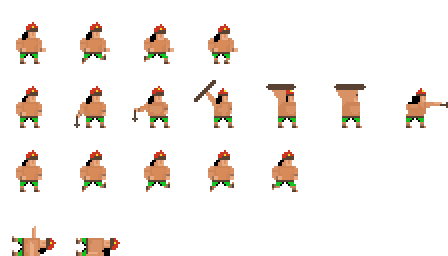
\includegraphics[scale=1.5]{player}
\centering
\caption{Sprites del personaje principal}
Elaborado por: Carlos Acuña
\end{figure}

\begin{figure}[h]
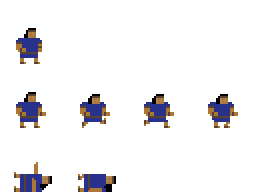
\includegraphics[scale=1.5]{enemy_warrior_blue}
\centering
\caption{Sprites NPC (enemigo)}
Elaborado por: Carlos Acuña
\end{figure}

\begin{figure}[h]
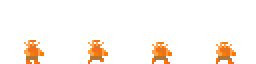
\includegraphics[scale=1.5]{apallimay}
\centering
\caption{Sprites NPC (bestia mitológica inca)}
Elaborado por: Carlos Acuña
\end{figure}

\begin{figure}[!]
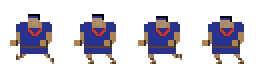
\includegraphics[scale=1.5]{chapera}
\centering
\caption{Sprites NPC (Jefe de nivel)}
Elaborado por: Carlos Acuña
\end{figure}
\clearpage
\item \textbf{Aspectos gráficos}\\
Es un juego totalmente en 2D que cuenta con una sola cámara que sigue al personaje principal, todos los objetos, personajes, terrenos y vistas están hechos en pixel art para dar al juego una imagen diferente y divertida.
\item \textbf{Interfaz de usuario}\\
En este apartado el jugador podrá realizar las principales acciones que permita realizar el juego, el cual se divide en n interfaces.
\begin{itemize}
\item \textbf{UI Logo.} Primera interfaz en mostrarse con el fin de presentar al creador del juego.
\item \textbf{UI Menu Principal.} Esta interfaz tendrá cuatro botones que son opciones que el jugador puede escoger como Comenzar Juego, escoger nivel, configuración y créditos.
\begin{figure}[h]
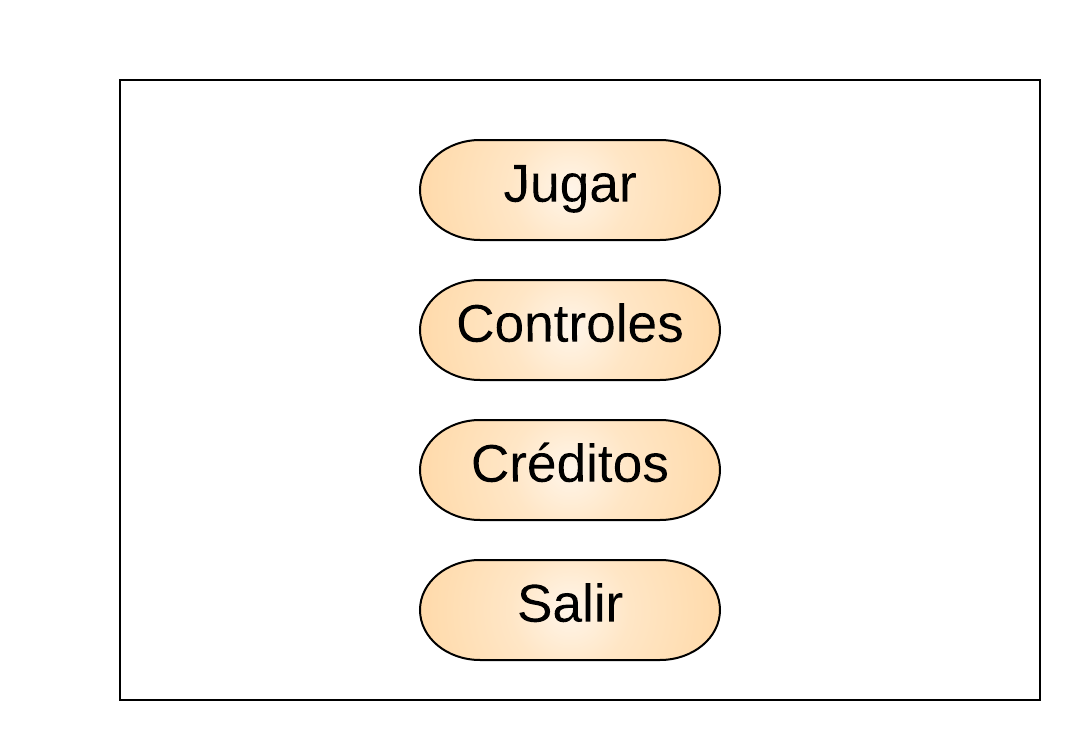
\includegraphics[scale=0.5]{ui_menu_principal}
\centering
\caption{UI Menú Principal}
Elaborado por: Carlos Acuña
\end{figure}

\item \textbf{UI Juego.} Aquí se mostrará la cantidad de vidas y puntos acumulados que el jugador tenga en ese nivel, además de ser la pantalla principal donde se ejecutará todas las acciones del jugador.

\item \textbf{UI Cinemática.} Esta interfaz se muestra en cada nivel como introducción donde se contará la historia con texto e imágenes para entender el transfondo de lo que está pasando en el juego.

\begin{figure}[h]
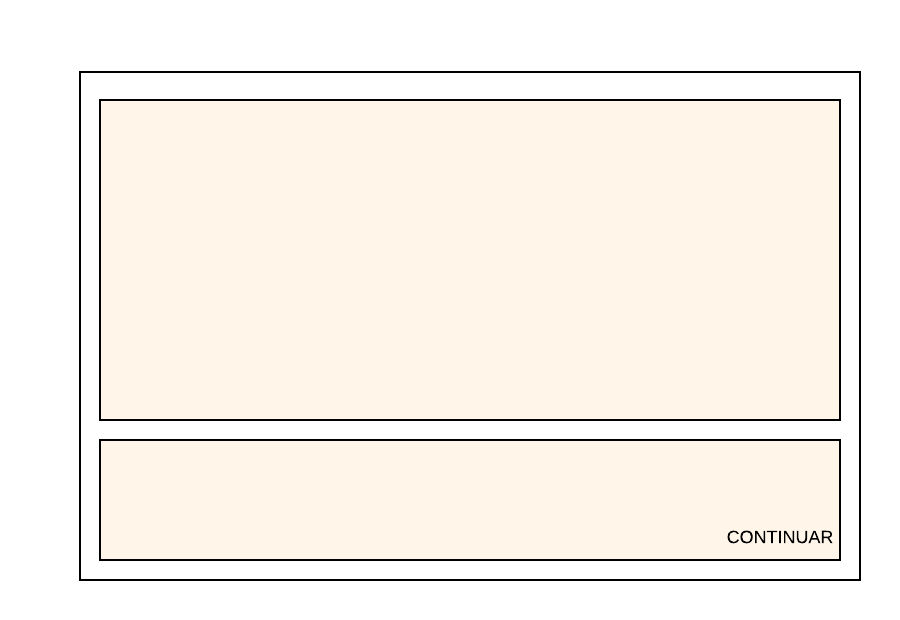
\includegraphics[scale=1]{ui_cinematica}
\centering
\caption{UI Cinemática}
Elaborado por: Carlos Acuña
\end{figure}
\end{itemize} 
\clearpage 
\item \textbf{Características de los elementos del videojuego}\\
En el cuadro \ref{t:elementosJuego} se describe los elementos principales del juego.
\begin{longtable}{| p{4cm} | p{6cm} |}
\hline
\captionsetup{justification=centering,margin=2cm}
%%Titulo
\textbf{Elementos} & \textbf{Descripción}\\ \hline
%%Contenido
Personaje Principal (Huaraca) & Se muestra al inicio de cada nivel donde realizará  acciones de acuerdo a los comandos ejecutados por el jugador con el fin de llegar al final del nivel \\ \hline
NPC (Enemigos) & Se muestran en todos los niveles con el fin de obstaculizar el paso del personajes principal, existen varios enemigos con diferentes acciones y movimientos \\ \hline
NPC (Jefes) & Se muestran al final de ciertos niveles con el fin de obstaculizar el paso del personajes principal, existen varios enemigos con diferentes acciones y movimientos, además de tener una cantidad mayor de puntos de vida \\ \hline
Interactivo (Corazón) & Da al personaje principal una vida adicional \\ \hline
Interactivo (Monedas de oro) & Al acumular una cierta cantidad de monedas de oro se gana una vida adicional\\ \hline
Interactivo (Checkpoint) & Elemento que permite guardar la posición actual del jugador y regresará a este punto en caso de perder una vida.\\ \hline
Interactivo (Choza) & Elemento donde al llegar se da por finalizado el nivel y comienza el siguiente\\ \hline
Peligros (Pinchos) & Son elementos que dañan al personaje principal si cruza con alguno de ellos haciendo perder una vida\\ \hline
Interactivo (Niveles) & Cada nivel creado es más complicado que el anterior y en algunos niveles aparece un jefe para dificultar el avance del jugador\\ \hline
\caption{Características de los elementos del videojuego}
\label{t:elementosJuego}
\end{longtable}

\begin{center}
Elaborado por: Carlos Acuña
\end{center}

\item \textbf{Objetivo del videojuego}\\
Enseñar sobre la cultura y mitología inca ecuatoriana de una manera divertida y amena a través de un videojuego que reta al jugador a completar niveles atravesando una serie de obstáculos que ponen a prueba sus habilidades y coordinación.\\
Cada nivel tiene como reto llegar del punto A al punto B con la mayor cantidad de vidas posibles en el menor tiempo posible para continuar con la aventura. 
\item \textbf{Reglas}\\
\begin{itemize}
\item Se inicia cada nivel con 1 vida(corazón) y cero monedas.
\item Cada nivel tiene enemigos y peligros que el jugador debe evitar o destruir para llegar al final del juego.
\item Al final de cada nivel el jugador debe llegar a una choza donde al ingresar por una puerta se acabará el nivel actual y comenzará el siguiente.
\item Si el jugador colisiona con un enemigo el jugador de inmediato muere y regresa al punto de partida o punto de chequeo (checkpoint).
\item Si el jugador colisiona con un peligro (pinchos) el jugador de inmediato muere y regresa al punto de partida o punto de chequeo (checkpoint).
\item Si el jugador pierde la misión la repite y todos los objetos obtenidos vuelven a su estado original, una vida (corazón) y 0 monedas.
\item El jugador puede disparar un proyectil que permite destruir a los enemigos.
\item Existen 3 subniveles por nivel y debe completarlos para continuar al siguiente nivel.
\end{itemize}
\end{enumerate}   

\subsection*{Aspectos técnicos}
\begin{enumerate}
\item \textbf{Requerimientos técnicos} 
\begin{longtable}{| p{5cm} | p{5cm} |}
\hline
%%Titulo
\textbf{Hardware} & \textbf{Software}\\ \hline
%%Contenido
Intel Core™ Duo o superior; OpenGL 3.0 compliant video card; 256 MB de RAM & Windows Vista o superior\\ \hline
\caption{Requisitos técnicos}
\end{longtable}
\begin{center}
Elaborado por: Carlos Acuña
\end{center}

\item \textbf{Arquitectura del videojuego}\\
La arquitectura que se utiliza es MVC(Modelo Vista Controlador) que es modelo con el que se trabaja en Unity.
\item \textbf{Diseño conceptual}
\begin{figure}[h]
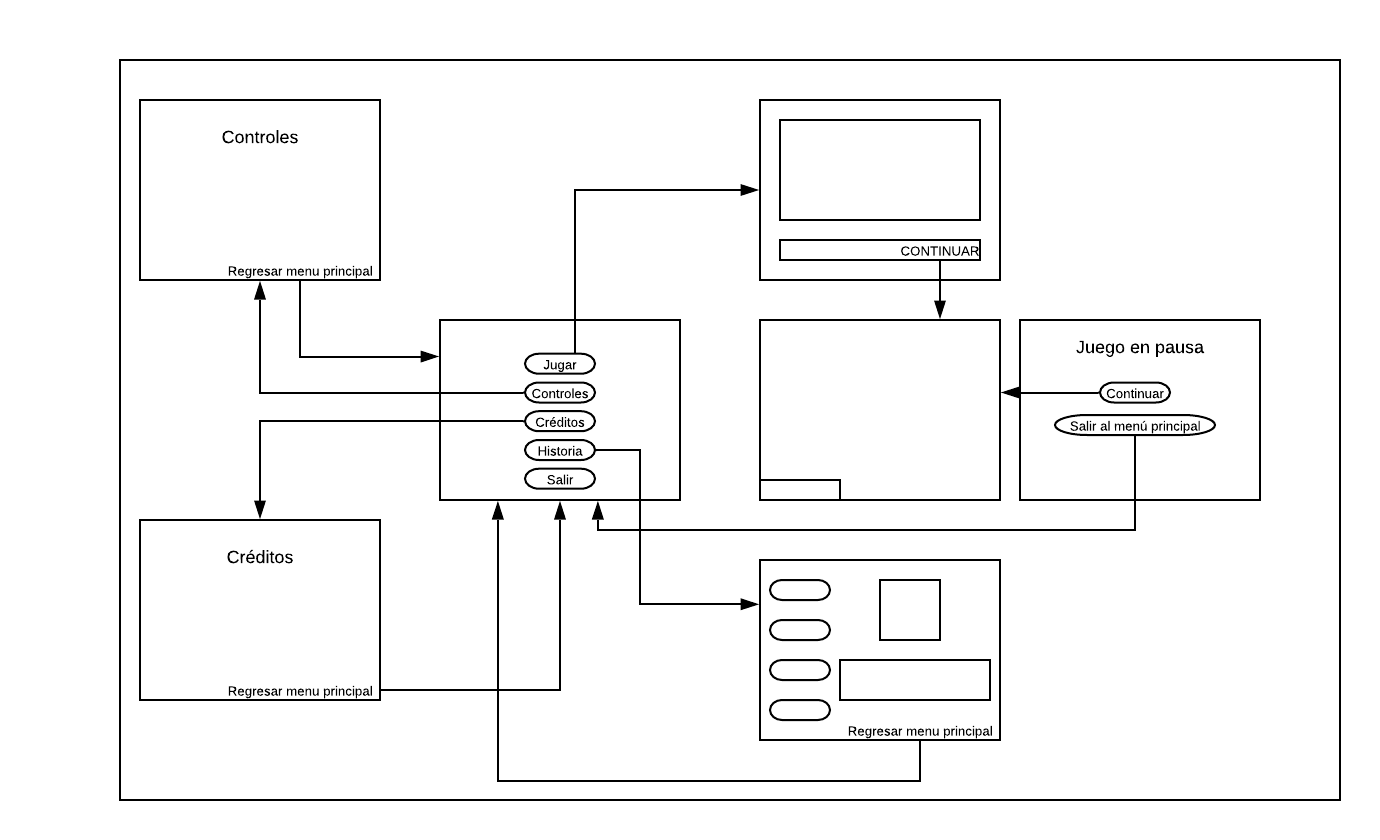
\includegraphics[scale=0.5]{concepto_juego}
\centering
\caption{Concepto del juego}
Elaborado por: Carlos Acuña
\end{figure}
\end{enumerate}

\subsection*{Herramientas a utilizarse}
\begin{itemize}
\item \textbf{Diseño gráfico}
\begin{itemize}
\item \textbf{GIMP.} GIMP es un acrónimo para (GNU Image Manipulation Program) o programa de manipulación de imágenes. Es un programa distribuido libremente para tareas como retoque de fotos, composición de imágenes y autorización de imágenes. GIMP tiene herramientas que se utilizan para el retoque y edición de imágenes, dibujo de formas libres, cambiar el tamaño, recortar, hacer fotomontajes, convertir a diferentes formatos de imagen, y otras tareas más especializadas. Se pueden también crear imágenes animadas en formato GIF e imágenes animadas en formato MPEG usando un plugin de animación. \cite{gimp2020}
\end{itemize}
\item \textbf{Desarrollo}
\begin{itemize}
\item \textbf{Visual Studio Code.} Visual Studio Code es un editor de código optimizado con soporte para operaciones de desarrollo como depuración, ejecución de tareas y control de versiones. Su objetivo es proporcionar solo las herramientas que un desarrollador necesita para un ciclo rápido de creación de código-depuración y deja flujos de trabajo más complejos para IDE más completos, como Visual Studio IDE. \cite{vsc2020}
\item \textbf{Unity3D.} Unity es un framework y motor de videojuegos multiplataforma creado por Unity Technologies. Unity está disponible como plataforma de desarrollo para Microsoft Windows, Mac OS, Linux y dispositivos móviles que permite la creación de videojuegos mediante la utilización de objetos que pueden ser importados hacia la herramienta, como son modelos 2D y 3D, archivos de texto, imágenes, sonidos, etc. Todo es hecho mediante varios lenguajes de programación como son BOO, C\# y Javascript. MonoDevelop es el IDE con el que trabaja Unity además de usar API's para el uso de rutinas, estructura de datos y clases, estas API's también son conocidas como librerías \cite{okita2014learning}.\\
Unity es completamente libre para cualquiera o cualquier empresa que gane menos de \$ 100000 al año, puede ser descargado sin ningún cargo adicional y sin tarjeta de crédito \cite{murray2014c}.
\end{itemize}
\end{itemize}

\subsection*{Roles de equipo}

\begin{table}[htb]
\centering
\begin{tabular}{|l|l|l|}
\hline
%%Titulo
\textbf{Persona} & \textbf{Contacto} & \textbf{Rol}\\ \hline
\multirow{5}{2cm}{Carlos Acuña} & \multirow{5}{4cm}{clsjs94@hotmail.com}  & DAV Master\\ \cline{3-3}
& & Dueño del producto \\ \cline{3-3}
& & Equipo DAV (Sonidista) \\ \cline{3-3}
& & Equipo DAV (Diseñador) \\ \cline{3-3}
& & Equipo DAV (Programador) \\ \cline{1-3}
\end{tabular}
\caption{Roles}
\end{table}
\begin{center}
Elaborado por: Carlos Acuña
\end{center}

\subsection*{Historias de usuarios}
\justify
Las historias de usuarios muestran el contenido y las funcionalidades que tendrá el videojuego "Huaraca".
\begin{longtable}{| l | l | p{5cm} | p{5cm} |}
\hline
%%Titulo
\textbf{ID} & \textbf{Como} & \textbf{Quiero.../Quiero que} & \textbf{De modo que.../Para} \\ \hline
%%Contenido
HU01 & Jugador &
Entrar, salir y ver los créditos del juego &
Entrar, salir y ver los créditos del juego \\ \hline
HU02 & Jugador &
Antes de cada nivel conocer el transfondo histórico y los personajes principales  &
Motivar a jugar el juego y aprender sobre historia ecuatoriana\\ \hline
HU03 & Jugador &
Visualizar los controles del juego &
Manejar los controles y mecánicas del juego \\ \hline
HU04 & Jugador &
Visualizar una pantalla de créditos &
Conocer a los creadores del videojuego\\ \hline
HU05 & Jugador &
Visualizar una pantalla que cuente el trasfondo histórico del juego &
Conocer la historia del juego \\ \hline
HU06 & Jugador &
Existan enemigos variados en cada nivel y puedan ser destruidos &
Mejorar la experiencia de juego \\ \hline
HU07 & Jugador &
Al final de cada nivel exista una batalla contra un jefe &
Aumentar la dificultad del juego \\ \hline
HU08 & Jugador &
Los niveles reflejen los paisajes andinos a través de pixel art &
Mejorar el aspecto visual del juego \\ \hline
HU09 & Jugador & 
Visualizar las vidas restantes y la puntuación actual &
Motivar al jugador a cambiar de estrategia según sus opciones \\ \hline
HU10 & Jugador &
La cámara siga al jugador en todo momento &
Tener una mejor visualización del juego \\ \hline
HU11 & Jugador &
El personaje principal cambie de animación según su acción &
El juego se vea más orgánico y dinámico \\ \hline
HU12 & Jugador &
Visualizar la meta de cada nivel &
Saber que se ha llegado al final de nivel del juego \\ \hline
HU13 & Jugador &
El personaje pierda el nivel cuando sus vidas lleguen a 0 &
Mantener la dificultad del juego \\ \hline
HU14 & Diseñador &
Los niveles tengan un fondo estilo pixel art &
Mejorar la calidad visual del juego \\ \hline 
HU15 & Sonidista &
Los efectos de sonido sean acordes a las acciones del jugador &
El juego sea más divertido \\ \hline
HU16 & Escritor &
Usar el recurso literario de la fantasía histórica &
Contar una historia entretenida pero basada en hechos reales \\ \hline
HU17 & Diseñador &
Agregar un story board en cada cambio de nivel &
Tener un recurso visual de los eventos que están ocurriendo \\ \hline
HU18 & Programador &
El personaje realice diferentes acciones  &
Permitir la interacción y progresión del juego \\ \hline
\caption{Historias de usuario del juego}
\end{longtable}
\begin{center}
Elaborado por: Carlos Acuña
\end{center}

\subsection*{Pruebas de aceptación}
\justify
Las pruebas de aceptación permiten validar las funcionalidades y características del videojuego una vez desarrolladas, de esta forma se garantiza que se cumpla con los requerimientos y pasaran a un estado de completado.

\begin{longtable}{| p{6cm} | p{6cm} |}
\hline
\multicolumn{2}{|c|}{\textbf{Prueba de tarea}} \\
\hline
\textbf{Identificador:} PA01 & \textbf{Historia de Usuario (Nro. y Nombre):} HU01 - Como jugador quiero entrar, salir y ver los créditos del juego \\
\hline
\multicolumn{2}{|p{12cm}|}{\textbf{Nombre:} Realizar el menú principal} \\ \hline
\multicolumn{2}{|p{12cm}|}{\textbf{Descripción:} Crear una interfaz con botones que permita entrar al juego y salir} \\ \hline
\multicolumn{2}{|p{12cm}|}{\textbf{Condiciones de ejecución:} Debe ejecutarse en cualquier tipo de pc, adaptarse a cualquier tipo de pantalla y funcionar correctamente} \\ \hline
\multicolumn{2}{|p{12cm}|}{\textbf{Entrada/Pasos de ejecución:} Presentar el menú principal con sus respectivos botones} \\ \hline
\multicolumn{2}{|p{12cm}|}{\textbf{Resultado esperado:} Acceder a las correspondientes interfaces según el botón seleccionado} \\ \hline
\caption{Prueba de aceptación PA01}
\end{longtable}
\begin{center}
Elaborado por: Carlos Acuña
\end{center}

\subsection*{Reserva del producto}
\justify
En el cuadro \ref{t: reservaP} se observan las historias de usuario con sus respectivas pruebas
de aceptación (PA), puntos de prioridad (P) y estimación (E) según el dueño
del producto.

\begin{longtable}{| l | l | p{5cm} | l | l | l |}
\hline
%%Titulo
\textbf{P} & \textbf{Nro. HU} & \textbf{Ítem} & \textbf{E} & \textbf{Estado} & \textbf{PA}\\ \hline
%%Contenido
3 & HU01 &
Entrar, salir y ver los créditos del juego &
1 & Pendiente & PA01 \\ \hline
2 & HU02 &
Antes de cada nivel conocer el transfondo histórico y los personajes principales  &
1 & Pendiente & PA02\\ \hline
3 & HU03 &
Visualizar los controles del juego &
1 & Pendiente & PA03 \\ \hline
3 & HU04 &
Visualizar una pantalla de créditos &
1 & Pendiente & PA04\\ \hline
3 & HU05 &
Visualizar una pantalla que cuente el trasfondo histórico del juego &
1 & Pendiente & PA05 \\ \hline
2 & HU06 &
Existan enemigos variados en cada nivel y puedan ser destruidos &
1 & Pendiente & PA06 \\ \hline
3 & HU07 &
Al final de cada nivel exista una batalla contra un jefe &
1 & Pendiente & PA07 \\ \hline
1 & HU08 &
Los niveles reflejen los paisajes andinos a través de pixel art &
1 & Pendiente & PA08 \\ \hline
2 & HU09 & 
Visualizar las vidas restantes y la puntuación actual &
1 & Pendiente & PA09 \\ \hline
1 & HU10 &
La cámara siga al jugador en todo momento &
1 & Pendiente & PA10 \\ \hline
1 & HU11 &
El personaje principal cambie de animación según su acción &
1 & Pendiente & PA11 \\ \hline
3 & HU12 &
Visualizar la meta de cada nivel &
1 & Pendiente & PA12 \\ \hline
2 & HU13 &
El personaje pierda el nivel cuando sus vidas lleguen a 0 &
1 & Pendiente & PA13 \\ \hline
1 & HU14 &
Los niveles tengan un fondo estilo pixel art &
1 & Pendiente & PA14 \\ \hline 
3 & HU15 &
Los efectos de sonido sean acordes a las acciones del jugador &
1 & Pendiente & PA15 \\ \hline
3 & HU16 &
Usar el recurso literario de la fantasía histórica &
1 & Pendiente & PA16 \\ \hline
3 & HU17 &
Agregar un story board en cada cambio de nivel &
1 & Pendiente & PA17 \\ \hline
1 & HU18 &
El personaje realice diferentes acciones  &
1 & Pendiente & PA18 \\ \hline
\caption{Historias de usuario del juego}
\label{t: reservaP}
\end{longtable}

\begin{center}
Elaborado por: Carlos Acuña
\end{center}

\subsection*{Determinación de las fechas de entrega}
\justify
Toda la reserva del producto se ha dividido en 4 iteraciones o entregas, con una duración de 1 mes cada una, las fechas de inicio y fin así como también las fechas de entrega de cada iteración.

\begin{longtable}{| l | l | l | l |}
\hline
%%Titulo
\textbf{Iteración} & \textbf{Fecha de inicio} & \textbf{Fecha de fin} & \textbf{Fecha de entrega} \\ \hline
%%Contenido
1 & 18 de diciembre del 2019 &
17 de enero del 2020 &
18 de enero del 2020 \\ \hline
2 & 19 de enero del 2020 &
17 de febrero del 2020 &
18 de febrero del 2020 \\ \hline
3 & 19 de febrero del 2020 &
17 de marzo del 2020 &
18 de marzo del 2020 \\ \hline
\caption{Fecha de entrega de cada iteración}
\end{longtable}
\begin{center}
Elaborado por: Carlos Acuña
\end{center}

\subsection{Fase de juego}
\justify
Una vez que se ha definido el alcance, las funcionalidades y un cronograma de las
fechas de entrega de cada iteración del videojuego se empezará el desarrollo de
cada una de las iteraciones.\\
En cada iteración se explica que historias de usuario se ha de implementar y se ha de comentar todos los pasos necesarios para llegar a cumplir los objetivos de esa etapa.\\ 
La duración de cada iteración será de 17 días es decir de lunes a sábado, los días
lunes se realizarán las reuniones de planificación de iteración y las revisiones de
las mismas se efectuarán los días domingos, de esta manera los otros días serán
usados para desarrollar las funcionalidades de cada entrega.

\subsection*{Desarrollo de la iteración 1}
\justify
El objetivo de esta iteración es obtener la primera versión del videojuego, la fecha de revisión de la iteración será el día 18 de enero de 2020, en esta iteración se desarrollará las siguientes historias de usuario.

\begin{longtable}{| l | p{5cm} |}
\hline
\captionsetup{justification=centering,margin=2cm}
%%Titulo
\textbf{ID} & \textbf{Descripción} \\ \hline
%%Contenido
HU08 &
Los niveles reflejen los paisajes andinos a través de pixel art \\ \hline
HU11 &
El personaje principal cambie de animación según su acción \\ \hline
HU19 &
El personaje realice diferentes acciones  \\ \hline
HU10 &
La cámara siga al jugador en todo momento \\ \hline
HU14 &
Los niveles tengan un fondo estilo pixel art \\ \hline 

\caption{Historias de usuario a implementarse en la Iteración 1}
\end{longtable}

\begin{center}
Elaborado por: Carlos Acuña
\end{center}

\justify
Se han generado tarjetas de tareas en base a las historias de usuarios seleccionadas para la iteración 1, las tareas fueron auto-asignadas al miembro del equipo DAV, el contenido de las tarjetas se encuentran en el Anexo A.\\
A continuación se resumen las tareas y subtareas realizadas para la iteración 1.

\subsection*{T01: Reflejar paisajes andinos mediante pixel art}
\justify
Para la creación de los paisajes se debe utilizar sprites, que mediante la herramienta Tilemap de Unity se pueden crear niveles para juegos de plataforma como del presente proyecto. Usando la herramienta Tilemap Pallete se dibuja el terreno, escaleras, peligros y objetos de fondo que se necesite para lograr crear el mapa en el cual el personaje deberá interactuar.\\
En la figura \ref{fig:T01_01} se muestra el resultado de usar el Tilemap para crear el primer nivel del juego.
   
\begin{figure}[h]
\centering
\captionsetup{justification=centering,margin=2cm}
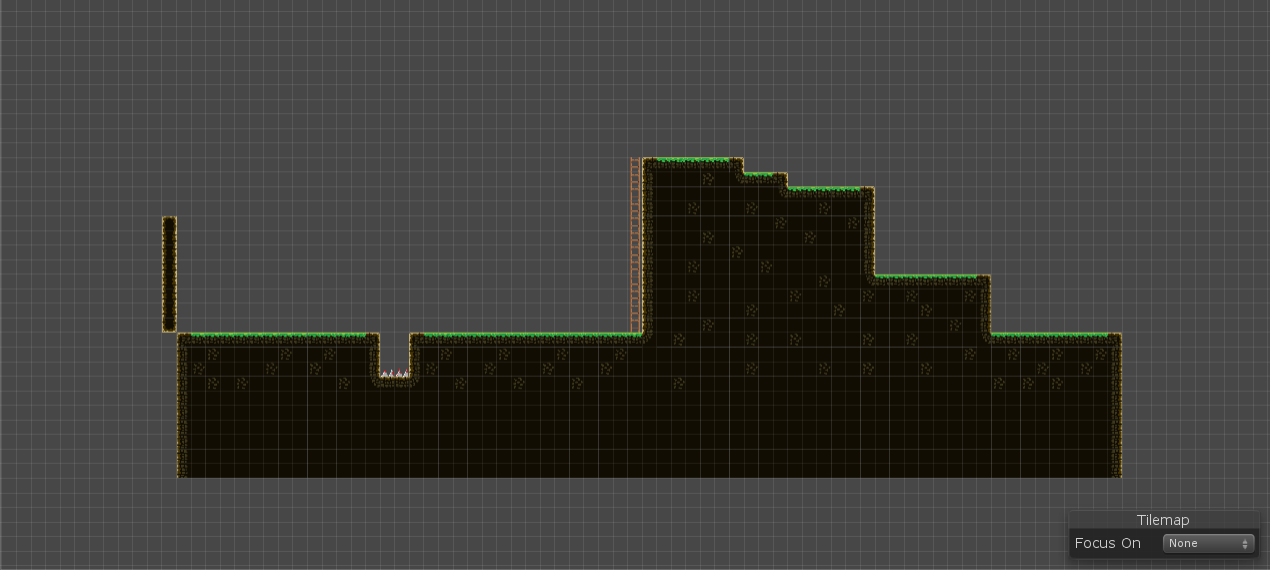
\includegraphics[scale=0.5]{T01_01}
\caption{Terreno creado con Tilemap}
Elaborado por: Carlos Acuña
\label{fig:T01_01}
\end{figure}
\clearpage
\justify
Cada terreno creado con Tilemap es diferente y depende de la dificultad del nivel  la extensión del mismo. Los sprites utilizados fueron creados con el fin de reflejar los terrenos de la cordillera de los Andes y toda la geografía que lo caracteriza pero en un estilo pixel art.

\subsection*{T02: El personaje principal cambie de animación según su acción}
\justify
Con el uso del programa GIMP se puede dibujar al personajes principal, donde cada imagen es un sprite. Los sprites del personaje principal se unen en una sola imagen conocida como spritesheet la cual contiene todas las posibles acciones que puede ocurrir en el juego como son estar quieto, correr, saltar, disparar y morir. En la figura \ref{fig:player} se muestra al personaje principal con sus acciones de movimiento.

\begin{figure}[h]
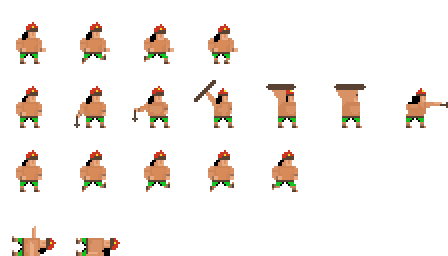
\includegraphics[scale=1.5]{player}
\centering
\caption{Sprites del personaje principal}
Elaborado por: Carlos Acuña
\label{fig:player}
\end{figure}

\justify
Para que el personaje cambie de animación se utiliza la herramienta Animation y Animator de Unity con el fin de crear animaciones basados en los sprites creados.  Se ha determinado 5 acciones acciones básicas del personaje principal como son estar quieto, correr, escalar, disparar y morir.\\
En la figura \ref{fig:T02_01} se muestra la creación de las animaciones con los sprites creados y en la figura \ref{fig:T02_02} se muestra la interacción de las animaciones de acuerdo al orden en que deben ser ejecutadas por cada acción que se realice.
\clearpage
\begin{figure}[h]
\captionsetup{justification=centering,margin=2cm}
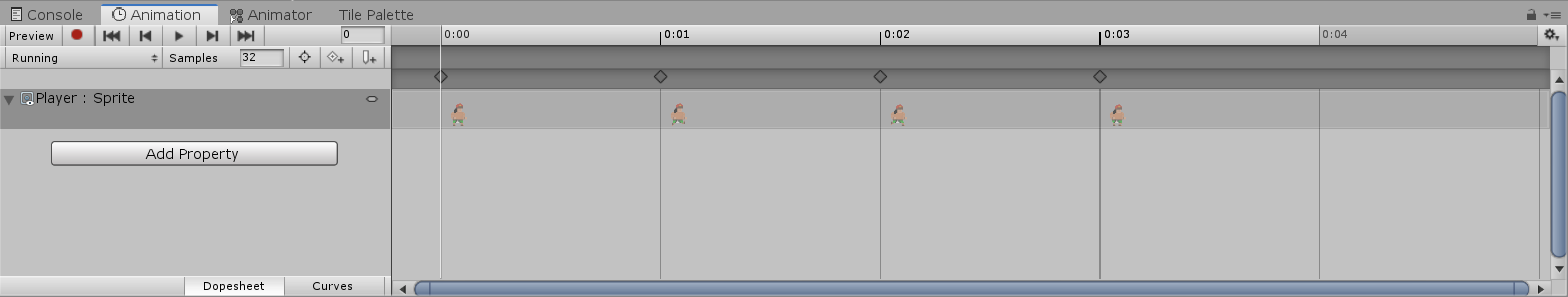
\includegraphics[scale=0.4]{T02_01}
\centering
\caption{Uso de la herramienta Animation para crear animaciones del personaje principal}
Elaborado por: Carlos Acuña
\label{fig:T02_01}
\end{figure}

\begin{figure}[h]
\captionsetup{justification=centering,margin=2cm}
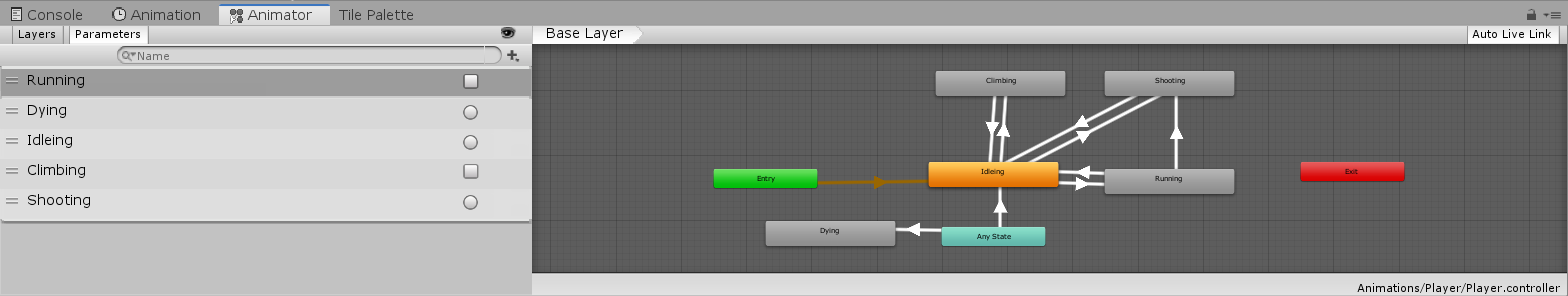
\includegraphics[scale=0.4]{T02_02}
\centering
\caption{Uso de la herramienta Animator para ordenar las animaciones del personaje principal}
Elaborado por: Carlos Acuña
\label{fig:T02_02}
\end{figure}
\clearpage
\subsection*{T03: El personaje realice diferentes acciones}
\justify
Dentro del videojuego se necesita que el personaje pueda interactuar con el terreno creado, para lo cual, acciones como correr, saltar, escalar y disparar son indispensables en este tipo de juego y son parte del objetivo de esta tarea. La clase que controlará todas estas acciones es la clase \textbf{``Player.cs"} junto con los métodos mostrados a continuación.

\begin{itemize}
\item \textbf{Correr.} La acción correr permite mover al personaje de izquierda a derecha y viceversa con el fin de que se mueva en todo el terreno hasta llegar a un punto concreto. El método encargado de esta acción se llama \textbf{``Run"}, el cual también se encarga de realizar la animación de correr al momento de llamar al método al presionar la tecla izquierda o derecha del teclado.

\begin{figure}[h]
\captionsetup{justification=centering,margin=2cm}
\centering
\lstset{language=C, breaklines=true, basicstyle=\footnotesize}
\lstset{numbers=left, numberstyle=\tiny, stepnumber=1, numbersep=-2pt}
\begin{lstlisting}[frame=single]
  private void Run()
    {
        float controlThrow = Input.GetAxis("Horizontal");
        Vector2 playerVelocity = new Vector2(controlThrow * runSpeed, myRigidbody.velocity.y);
        myRigidbody.velocity = playerVelocity;

        bool playerHasHorizontalSpeed = Mathf.Abs(myRigidbody.velocity.x) > Mathf.Epsilon;
        myAnimator.SetBool("Running", playerHasHorizontalSpeed);
    }
\end{lstlisting}
\caption{Método ``Run"}
Elaborado por: Carlos Acuña
\end{figure}

Para que el personaje cambie de vista en el escenario dependiendo de que si ve hacia la derecha o izquierda se utiliza el método \textbf{``FlipSprite"} que permite esta acción al momento que el personaje se pone en movimiento dándole una visión más realista a la animación.

\begin{figure}[h]
\captionsetup{justification=centering,margin=2cm}
\centering
\lstset{language=C, breaklines=true, basicstyle=\footnotesize}
\lstset{numbers=left, numberstyle=\tiny, stepnumber=1, numbersep=-2pt}
\begin{lstlisting}[frame=single]
  private void FlipSprite()
    {
        if (myRigidbody.velocity.x > 0f && !lookRight)
        {
            transform.Rotate(0f, 180f, 0f);
            lookRight = true;
        }
        else if (myRigidbody.velocity.x < 0f && lookRight)
        {
            transform.Rotate(0f, 180f, 0f);
            lookRight = false;
        }
    }
\end{lstlisting}
\caption{Método ``FlipSprite"}
Elaborado por: Carlos Acuña
\end{figure}

\item \textbf{Saltar.} La acción saltar permite mover al personaje principal de arriba hacia abajo simulando un salto en el cual el personaje detecta el terreno, si hay terreno puede ejecutar el salto caso contrario el jugador no podrá ejecutar más saltos hasta que el personaje toque el suelo nuevamente, para ejecutar esta acción se presiona la tecla arriba del teclado. Cabe destacar que la gravedad es importante para que la simulación del salto sea correcta por lo cual este parámetro se modifica en las opciones de proyectos de Unity.\\
El método encargado de esta acción es el método \textbf{``Jump"}

\begin{figure}[h]
\captionsetup{justification=centering,margin=2cm}
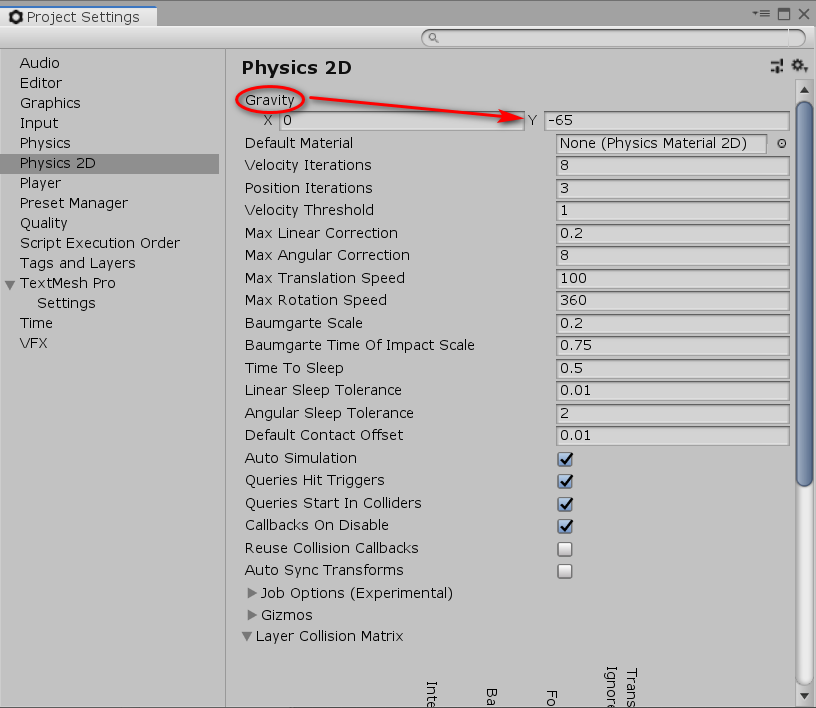
\includegraphics[scale=0.3]{T03_01}
\centering
\caption{Uso de las opciones de proyecto para modificar la gravedad de los objetos del juego}
Elaborado por: Carlos Acuña
\label{fig:T03_01}
\end{figure}

\begin{figure}[h]
\captionsetup{justification=centering,margin=2cm}
\centering
\lstset{language=C, breaklines=true, basicstyle=\footnotesize}
\lstset{numbers=left, numberstyle=\tiny, stepnumber=1, numbersep=-2pt}
\begin{lstlisting}[frame=single]
  private void Jump()
    {
        if (!myFeetCollider2D.IsTouchingLayers(LayerMask.GetMask("Foreground"))) { return; }

        if (Input.GetButtonDown("Jump"))
        {
            Vector2 jumpVelocityToAdd = new Vector2(0f, jumpSpeed);
            AudioSource.PlayClipAtPoint(jumpSFX, Camera.main.transform.position);
            myRigidbody.velocity += jumpVelocityToAdd;
        }
    }
\end{lstlisting}
\caption{Método ``Jump"}
Elaborado por: Carlos Acuña
\end{figure}

\item \textbf{Escalar.} La acción escalar permite simular la subida del personaje   al momento de colisionar con el elemento del terreno conocido como escaleras, esto con el fin de alcanzar grandes alturas que no pueden ser atravesados con la función salto. Se utiliza la tecla arriba del teclado para realizar esta acción y debido a las colisión con el elemento escaleras se evita que el personaje se confunda con la acción de saltar. El método encargado de esta función es \textbf{``ClimbLadder"}.

\begin{figure}[h]
\captionsetup{justification=centering,margin=2cm}
\centering
\lstset{language=C, breaklines=true, basicstyle=\footnotesize}
\lstset{numbers=left, numberstyle=\tiny, stepnumber=1, numbersep=-2pt}
\begin{lstlisting}[frame=single]
  private void ClimbLadder()
    {
        if (!myFeetCollider2D.IsTouchingLayers(LayerMask.GetMask("Climbing")))
        {
            myAnimator.SetBool("Climbing", false);
            myRigidbody.gravityScale = gravityScaleAtStart;
            return;
        }

        float controlThrow = Input.GetAxis("Vertical");
        Vector2 climbVelocity = new Vector2(myRigidbody.velocity.x, controlThrow * climbSpeed);
        myRigidbody.velocity = climbVelocity;
        myRigidbody.gravityScale = 0f;

        bool playerHasVerticalSpeed = Mathf.Abs(myRigidbody.velocity.y) > Mathf.Epsilon;
        myAnimator.SetBool("Climbing", playerHasVerticalSpeed);
    }
\end{lstlisting}
\caption{Método ``ClimbLadder"}
Elaborado por: Carlos Acuña
\end{figure}
\clearpage
\item \textbf{Disparar.} Como el nombre lo indica, esta acción permite la destrucción de los enemigos que aparezcan en cada nivel, tanto enemigos normales como jefes de nivel, esta acción consta de dos métodos. El primer método \textbf{``CanShoot"} que da un tiempo de espera entre cada disparo para que exista una saturación de proyectiles en pantalla al momento de realizar esta acción y el método \textbf{``Shoot"} que realiza la acción de disparar, junto con la animación del personaje que está disparando y la instanciación del proyectil que al momento de chocar con un enemigo, este será destruido y desaparecerá de la pantalla. Esta acción se realiza presionando la tecla ``x" del teclado.

\begin{figure}[h]
\captionsetup{justification=centering,margin=2cm}
\centering
\lstset{language=C, breaklines=true, basicstyle=\footnotesize}
\lstset{numbers=left, numberstyle=\tiny, stepnumber=1, numbersep=-2pt}
\begin{lstlisting}[frame=single]
  private bool CanShoot()
    {
        return Time.time > this.waitingShoot;
    }
\end{lstlisting}
\caption{Método ``CanShoot"}
Elaborado por: Carlos Acuña
\end{figure}

\begin{figure}[h]
\captionsetup{justification=centering,margin=2cm}
\centering
\lstset{language=C, breaklines=true, basicstyle=\footnotesize}
\lstset{numbers=left, numberstyle=\tiny, stepnumber=1, numbersep=-2pt}
\begin{lstlisting}[frame=single]
  private void Shoot()
    {
        float fire = Input.GetAxis("Fire1");
        if (fire != 0f && CanShoot())
        {
            myAnimator.SetTrigger("Shooting");
            AudioSource.PlayClipAtPoint(throwSFX, Camera.main.transform.position);
            Instantiate(prefabProjectile, firePoint.position, firePoint.rotation);
            waitingShoot = Time.time + timingShoot;
        }
    }
\end{lstlisting}
\caption{Método ``Shoot"}
Elaborado por: Carlos Acuña
\end{figure}
\end{itemize} 
\clearpage
\subsection*{T04: La cámara sigue al jugador en todo momento}
\justify
Aquí se busca que la pantalla siga los movimientos del personaje principal en todo el videojuego con el fin de que el jugador no se pierda al momento de realizar cualquier tipo de acción y que todo lo que ocurra cerca del personaje se vea de manera clara y concisa siempre centrado en el jugador. Para esto se ha de usar una herramienta de Unity conocida como \textbf{``Cinemachine"} que permite la manipulación de la cámara de manera fácil e intuitiva de manejar, adaptándose a las necesidades del juego.\\
Para crear una cámara de este tipo se necesita añadir esta herramienta al proyecto de Unity, luego se añadirá dos nuevas cámaras virtuales, una para cuando el personaje principal está quieto en la pantalla y otra cuando comience a realizar cualquier movimiento. Estas cámaras tendrán varios elementos que ayudarán a mejorar el seguimiento del jugador y dar una experiencia más pulida al momento de interactuar con el juego.

\begin{figure}[h]
\captionsetup{justification=centering,margin=2cm}
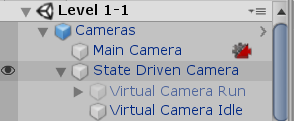
\includegraphics[scale=1]{T04_01}
\centering
\caption{Ventana de jerarquía donde se encuentran las cámaras virtuales}
Elaborado por: Carlos Acuña
\label{fig:T04_01}
\end{figure}

\begin{figure}[h]
\captionsetup{justification=centering,margin=2cm}
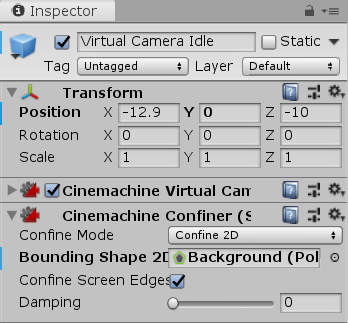
\includegraphics[scale=1]{T04_02}
\centering
\caption{Ventana del Inspector de la cámara Idle}
Elaborado por: Carlos Acuña
\label{fig:T04_02}
\end{figure}

\begin{figure}[h]
\captionsetup{justification=centering,margin=2cm}
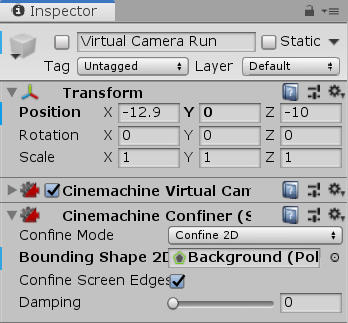
\includegraphics[scale=1]{T04_03}
\centering
\caption{Ventana del Inspector de la cámara Run}
Elaborado por: Carlos Acuña
\label{fig:T04_03}
\end{figure}
\clearpage
\subsection*{T05: Los niveles tengan un fondo estilo pixel art}
\justify
Para la creación de los fondos se ha recurrido a la búsqueda de escenarios que tengan relación con el paisaje andino, para lo cual se encontró unos fondos de pantalla creados específicamente para videojuegos, los cuales cumplen con las condiciones necesarias para adaptarse al estilo de juego que se está creando.
Estos fondos de pantalla se encontraron en la siguiente página web: https://vnitti.itch.io/grassy-mountains-parallax-background de manera gratuita y para su uso libre en cualquier proyecto relacionado con videojuegos.

\begin{figure}[h]
\captionsetup{justification=centering,margin=2cm}
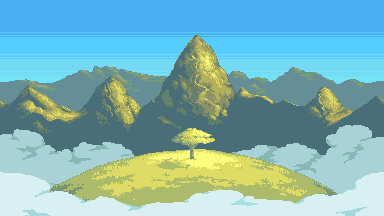
\includegraphics[scale=1]{T05_01}
\centering
\caption{Previsualización de los fondos de pantalla en pixel art}
Elaborado por: vnitti
\label{fig:T05_01}
\end{figure}

\subsection*{Entrega funcional de la iteracion 1}
\justify
La primera iteración para el 17 de enero del 2020 fue completada con éxito de acuerdo a la planificación que se había planeado.\\
Como resultado se obtuvo que el personaje principal está en pantalla sobre el terreno construido en pixel art. Las acciones correr, saltar, disparar y escalar son funcionales y es fondo de pantalla del juego representa lo más fielmente a la geografía andina. La figura \ref{fig:I01_01} muestra el resultado final de la iteración 1.

\begin{figure}[h]
\captionsetup{justification=centering,margin=2cm}
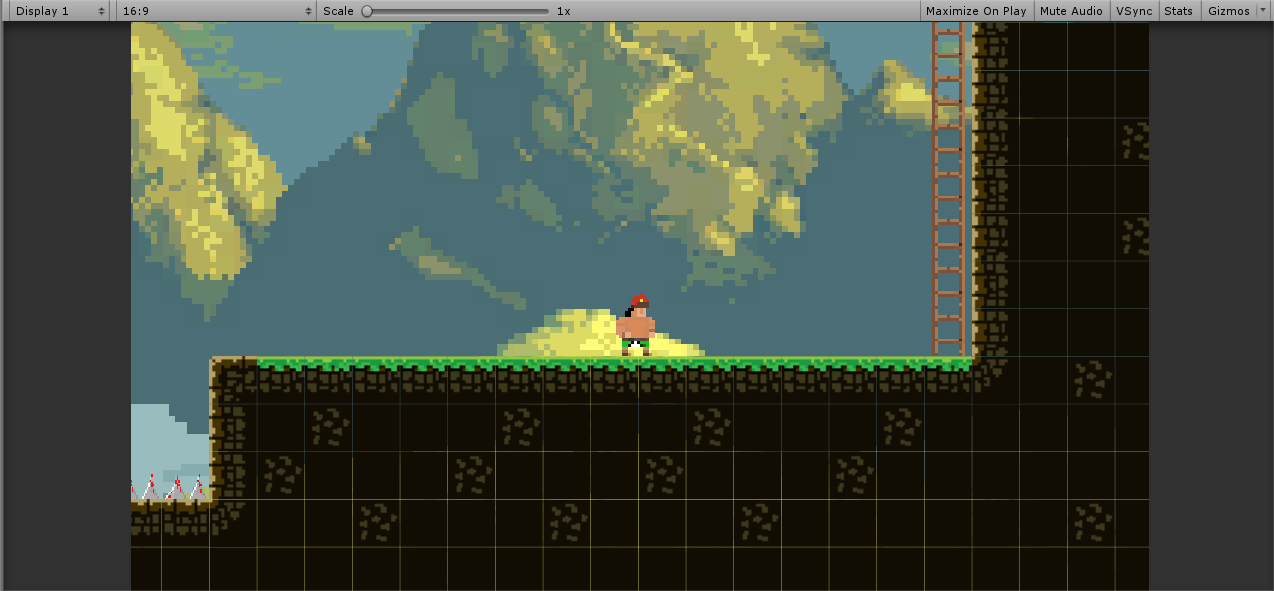
\includegraphics[scale=0.4]{I01_01}
\centering
\caption{Resultado de la iteración 1}
Elaborado por: Carlos Acuña
\label{fig:I01_01}
\end{figure}
\clearpage
\subsection*{Desarrollo de la iteración 2}
\justify
El objetivo de esta iteración es obtener la segunda versión del videojuego, la fecha de revisión de la iteración será el día 18 de febrero de 2020, en esta iteración se desarrollará las siguientes historias de usuario.

\begin{longtable}{| l | p{5cm} |}
\hline
\captionsetup{justification=centering,margin=2cm}
%%Titulo
\textbf{ID} & \textbf{Descripción} \\ \hline
%%Contenido
HU09 &
Visualizar las vidas restantes y la puntuación actual \\ \hline
HU13 &
El personaje pierda el nivel cuando sus vidas lleguen a 0 \\ \hline
HU06 &
Existan enemigos variados en cada nivel y puedan ser destruidos\\ \hline
HU02 &
Antes de cada nivel conocer el transfondo histórico y los personajes principales \\ \hline
\caption{Historias de usuario a implementarse en la Iteración 2}
\end{longtable}
\begin{center}
Elaborado por: Carlos Acuña
\end{center}
\justify
Se han generado tarjetas de tareas en base a las historias de usuarios seleccionadas para la iteración 2, las tareas fueron auto-asignadas al miembro del equipo DAV, el contenido de las tarjetas se encuentran en el Anexo A.\\
A continuación se resumen las tareas y subtareas realizadas para la iteración 2.

\subsection*{T06: Visualizar las vidas restantes y la puntuación actual}
\justify
Para visualizar las vidas y puntuación se debe tener en cuenta que se necesitan varias partes para que funcionen de manera correcta, estos elementos son:
\begin{itemize}
\item \textbf{Creación de la clase ``LevelManager.cs".} La clase \textbf{``LevelManager.cs"} es la clase encargada de llevar los datos de salud y puntuación, guardar información importante del nivel, añadir las vidas extras y la cantidad de monedas de oro y controlar la acción de muerte del personaje principal.\\
Los primeros métodos que se crean en esta clase son \textbf{``AddLives"} que permiten añadir una vida adicional al personaje principal y el método \textbf{``AddCoins"}que permite que se añada también una vida adicional cada conteo de 100 monedas de oro, este último método funciona conjuntamente con el método \textbf{``Update"} de la clase.

\begin{figure}[h]
\captionsetup{justification=centering,margin=2cm}
\centering
\lstset{language=C, breaklines=true, basicstyle=\footnotesize}
\lstset{numbers=left, numberstyle=\tiny, stepnumber=1, numbersep=-2pt}
\begin{lstlisting}[frame=single]
  public void AddLives(int livesToAdd)
  {
        currentLives += livesToAdd;
        livesText.text = "x " + currentLives;
  }
\end{lstlisting}
\caption{Método ``AddLives"}
Elaborado por: Carlos Acuña
\end{figure}

\begin{figure}[h]
\captionsetup{justification=centering,margin=2cm}
\centering
\lstset{language=C, breaklines=true, basicstyle=\footnotesize}
\lstset{numbers=left, numberstyle=\tiny, stepnumber=1, numbersep=-2pt}
\begin{lstlisting}[frame=single]
  public void AddCoins(int coinToAdd)
  {
        coinCount += coinToAdd;
        coinBonusLifeCount += coinToAdd;
        coinText.text = "x " + coinCount.ToString();
  }
\end{lstlisting}
\caption{Método ``AddCoins"}
Elaborado por: Carlos Acuña
\end{figure}

\begin{figure}[h]
\captionsetup{justification=centering,margin=2cm}
\centering
\lstset{language=C, breaklines=true, basicstyle=\footnotesize}
\lstset{numbers=left, numberstyle=\tiny, stepnumber=1, numbersep=-2pt}
\captionsetup{justification=centering,margin=2cm}
\begin{lstlisting}[frame=single]
  void Update()
  {
        if (coinBonusLifeCount >= 100)
        {
            currentLives += 1;
            livesText.text = "x " + currentLives;
            coinBonusLifeCount -= 100;
        }
  }
\end{lstlisting}
\caption{Método ``Update" para aumentar el número de vidas por conteo de monedas de oro}
Elaborado por: Carlos Acuña
\end{figure}
\clearpage
\item \textbf{Utilización de PlayerPrefs.} Para que se pueda guardar los datos relevantes sobre el juego se necesita usar la herramienta \textbf{``PlayerPrefs"} de Unity que permite guardar elementos como números y letras y otro tipo de información, estos datos permiten que funcionen correctamente otras mecánicas del juego. Estos datos se llaman desde el método \textbf{``Start"} que no solo funcionan en el nivel actual, sino que estos datos están presenten en todo el videojuego, todo se reinicia al momento de iniciar una nueva partida.

\begin{figure}[h]
\captionsetup{justification=centering,margin=2cm}
\centering
\lstset{language=C, breaklines=true, basicstyle=\footnotesize}
\lstset{numbers=left, numberstyle=\tiny, stepnumber=1, numbersep=-2pt}
\captionsetup{justification=centering,margin=2cm}
\begin{lstlisting}[frame=single]
  void Start()
  {
        player = FindObjectOfType<Player>();

        if (PlayerPrefs.HasKey("coinCount"))
        {
            coinCount = PlayerPrefs.GetInt("coinCount");
        }

        coinText.text = "x " + coinCount.ToString();

        if (PlayerPrefs.HasKey("playerLives"))
        {
            currentLives = PlayerPrefs.GetInt("playerLives");
        }
        else
        {
            currentLives = startingLives;
        }

        livesText.text = "x " + currentLives;
  }
\end{lstlisting}
\caption{Método ``Start' con los componentes ``PlayerPrefs" para guardar información}
Elaborado por: Carlos Acuña
\end{figure}

\begin{figure}[h]
\captionsetup{justification=centering,margin=2cm}
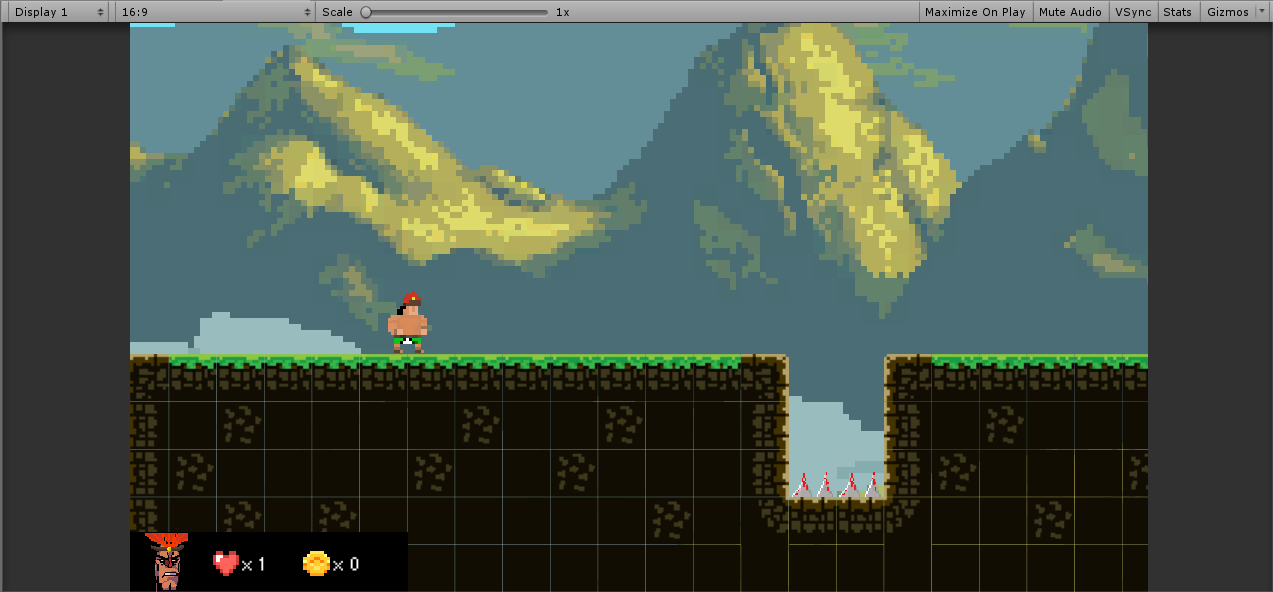
\includegraphics[scale=0.5]{T06_01}
\centering
\caption{Imagen del juego con los datos de vida y monedas de oro}
Elaborado por: Carlos Acuña
\label{fig:T06_01}
\end{figure}
\clearpage
\item \textbf{Creación de los ``GameObject" para vidas y monedas de oro.} Para que el personaje pueda ganar sus vidas y monedas dentro del juego, se necesita la creación de objetos que puedan ser usados para ese fin, es aquí donde se requiere el uso de \textbf{``GameObject"}. Estos objetos de juego son elementos que se encontrarán en la mayoría de niveles y ejecutarán eventos una vez que el jugador colisione con estos. Para que estos eventos funcionen se ha creado las clases \textbf{``ExtraLife.cs"} y \textbf{``Coin.cs"} con su respectivos métodos de colisión, el cual es \textbf{``OnTriggerEnter2D"}. Este método permite detectar colisiones del jugador y se ejecute el evento de añadir vidas o añadir monedas que se crearon en la clase \textbf{``LevelManager.cs"}.

\begin{figure}[h]
\captionsetup{justification=centering,margin=2cm}
\centering
\lstset{language=C, breaklines=true, basicstyle=\footnotesize}
\lstset{numbers=left, numberstyle=\tiny, stepnumber=1, numbersep=-2pt}
\captionsetup{justification=centering,margin=2cm}
\begin{lstlisting}[frame=single]
  private void OnTriggerEnter2D(Collider2D other)
  {
        if (other.tag == "Player")
        {
            AudioSource.PlayClipAtPoint(healthPickUpSFX, Camera.main.transform.position);
            levelManager.AddLives(livesToGive);
            Destroy(gameObject);
        }
  }
\end{lstlisting}
\caption{Método ``OnTriggerEnter2D" de la clase ``ExtraLife.cs"}
Elaborado por: Carlos Acuña
\end{figure}

\begin{figure}[h]
\captionsetup{justification=centering,margin=2cm}
\centering
\lstset{language=C, breaklines=true, basicstyle=\footnotesize}
\lstset{numbers=left, numberstyle=\tiny, stepnumber=1, numbersep=-2pt}
\captionsetup{justification=centering,margin=2cm}
\begin{lstlisting}[frame=single]
  private void OnTriggerEnter2D(Collider2D other)
  {

        if (other.tag == "Player")
        {
            AudioSource.PlayClipAtPoint(coinPickUpSFX, Camera.main.transform.position);
            levelManager.AddCoins(coinValue);
            Destroy(gameObject);
        }
  }
\end{lstlisting}
\caption{Método ``OnTriggerEnter2D" de la clase ``Coin.cs"}
Elaborado por: Carlos Acuña
\end{figure}

\end{itemize}

\subsection*{T07: El personaje pierde el nivel cuando sus vidas llegan a 0}
\justify
En este apartado el objetivo es añadir dificultad al juego mediante el sistema de vidas creada en la tarea T06, al permitir que se pierda el nivel cuando las vidas del personaje principal llegue a 0. Para esto se debe tomar en cuenta que hay varias subtareas que realizar, así tenemos:

\begin{itemize}

\item \textbf{Creación de un Checkpoint.} Los checkpoints o puntos de control son elementos que permiten en un juego regresar a un estado anterior en un punto concreto del mapa. Esto se justifica debido a que si pierde una vida, no necesariamente pierde el nivel, ya que el contador de vidas puede mayor a uno y por lo tanto no sería justo para el jugador volver a empezar todo de nuevo pero eso no quita la penalización por perder en esa parte del nivel.\\
El checkpoint funciona al momento en que el personaje principal choca con el \textbf{``GameObject"} conocido como checkpoint y se activa un evento mediante el método \textbf{``OnTriggerEnter2D"} de la clase \textbf{``Player"}. Este evento guarda la posición actual del personaje y tendrá una animación para confirmar que se ha realizado la acción mediante la clase \textbf{``Checkpoint"}.

\begin{figure}[h]
\captionsetup{justification=centering,margin=2cm}
\centering
\lstset{language=C, breaklines=true, basicstyle=\footnotesize}
\lstset{numbers=left, numberstyle=\tiny, stepnumber=1, numbersep=-2pt}
\captionsetup{justification=centering,margin=2cm}
\begin{lstlisting}[frame=single]
  private void OnTriggerEnter2D(Collider2D other)
    {
        if (other.tag == "Checkpoint")
        {
            respawnPosition = other.transform.position;
        }
    }
\end{lstlisting}
\caption{Método ``OnTriggerEnter2D" de la clase ``Player.cs"}
Elaborado por: Carlos Acuña
\end{figure}

\begin{figure}[h]
\captionsetup{justification=centering,margin=2cm}
\centering
\lstset{language=C, breaklines=true, basicstyle=\footnotesize}
\lstset{numbers=left, numberstyle=\tiny, stepnumber=1, numbersep=-2pt}
\captionsetup{justification=centering,margin=2cm}
\begin{lstlisting}[frame=single]
  private void OnTriggerEnter2D(Collider2D other)
    {
        if (other.tag == "Player")
        {
            checkpointActive = true;
            fire.SetActive(true);
        }
    }
\end{lstlisting}
\caption{Método ``OnTriggerEnter2D" de la clase ``Checkpoint.cs"}
Elaborado por: Carlos Acuña
\end{figure}

\item \textbf{Acción morir del personaje.} Para que el personaje principal pierda el nivel debe exponerse a varios peligros como al chocar con ciertos elementos del terreno que puedan dañarlo o al toparse con algunos enemigos que impidan su paso.\\
Para esto se ha creado subrutinas que permiten la simulación de la acción morir del personaje principal dividiendo en dos partes, la primera se crea el método \textbf{``ProcessPlayerDeath"} que es cuando muere pero aún le quedan vidas de sobra y reaparece en el último checkpoint del mapa y el otro método es \textbf{``ProcessPlayerRestart"} cuando ya no le queda ninguna vida y se debe reiniciar totalmente el nivel. Estos métodos deben ser llamados en el método \textbf{``Respawn"} de la clase \textbf{``LevelManager"}. 

\begin{figure}[h]
\captionsetup{justification=centering,margin=2cm}
\centering
\lstset{language=C, breaklines=true, basicstyle=\footnotesize}
\lstset{numbers=left, numberstyle=\tiny, stepnumber=1, numbersep=-2pt}
\captionsetup{justification=centering,margin=2cm}
\begin{lstlisting}[frame=single]
  public IEnumerator ProcessPlayerDeath()
    {
        player.GetComponent<Animator>().SetTrigger("Dying");
        player.isAlive = false;
        Instantiate(deathExplosion, player.transform.position, player.transform.rotation);
        yield return new WaitForSeconds(waitToRespawn);
        player.isAlive = true;
        coinCount = 0;
        coinText.text = "x " + coinCount.ToString();
        coinBonusLifeCount = 0;
        player.transform.position = player.respawnPosition;
        player.GetComponent<Animator>().SetTrigger("Idleing");
    }
\end{lstlisting}
\caption{Método ``ProcessPlayerDeath" de la clase ``LevelManager.cs"}
Elaborado por: Carlos Acuña
\end{figure}

\begin{figure}[h]
\captionsetup{justification=centering,margin=2cm}
\centering
\lstset{language=C, breaklines=true, basicstyle=\footnotesize}
\lstset{numbers=left, numberstyle=\tiny, stepnumber=1, numbersep=-2pt}
\captionsetup{justification=centering,margin=2cm}
\begin{lstlisting}[frame=single]
  public IEnumerator ProcessPlayerRestart()
    {
        player.gameObject.SetActive(false);
        gameOverScreen.SetActive(true);
        levelMusic.Stop();
        gameOverMusic.Play();
        yield return new WaitForSeconds(waitToRestart);
        var currentSceneIndex = SceneManager.GetActiveScene().buildIndex;
        SceneManager.LoadScene(currentSceneIndex);
    }
\end{lstlisting}
\caption{Método ``ProcessPlayerRestart" de la clase ``LevelManager.cs"}
Elaborado por: Carlos Acuña
\end{figure}

\begin{figure}[h]
\captionsetup{justification=centering,margin=2cm}
\centering
\lstset{language=C, breaklines=true, basicstyle=\footnotesize}
\lstset{numbers=left, numberstyle=\tiny, stepnumber=1, numbersep=-2pt}
\captionsetup{justification=centering,margin=2cm}
\begin{lstlisting}[frame=single]
  public void Respawn()
    {
        currentLives -= 1;
        livesText.text = "x " + currentLives;
        if (currentLives > 0)
        {
            StartCoroutine("ProcessPlayerDeath");
        }
        else
        {
            StartCoroutine("ProcessPlayerRestart");
        }
    }
\end{lstlisting}
\caption{Método ``Respawn" de la clase ``LevelManager.cs"}
Elaborado por: Carlos Acuña
\end{figure}

\end{itemize}
\clearpage
\subsection*{T08: Existan enemigos variados en cada nivel y puedan ser destruidos}
\justify
En todo juego de plataformas debe existir la figura del enemigo con el fin de obstaculizar el progreso del personaje principal, en este apartado se creado varios tipos de enemigos, ya sean humanos o bestias mitológicas.\\
Primero se debe diseñar los modelos de los enemigos que serán usados para la animación de cada NPC y su respectiva clase para su funcionamiento.

\begin{itemize}
\item \textbf{Creación de los enemigos.} Para crear a los enemigos se los diseñó en la herramienta GIMP, basados en guerreros de la época y bestias mitológicas incas, a los cuales se les ha dado un diseño pixel art, así tenemos:

\begin{figure}[h]
\captionsetup{justification=centering,margin=2cm}
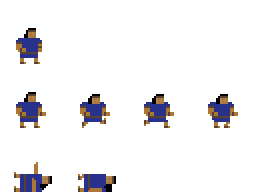
\includegraphics[scale=3]{T08_01}
\centering
\caption{NPC (Guerrero)}
Elaborado por: Carlos Acuña
\label{fig:T08_01}
\end{figure}

\begin{figure}[h]
\captionsetup{justification=centering,margin=2cm}
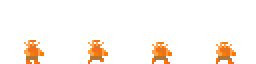
\includegraphics[scale=3]{T08_02}
\centering
\caption{NPC (Apallimay)}
Elaborado por: Carlos Acuña
\label{fig:T08_02}
\end{figure}

\begin{figure}[!]
\captionsetup{justification=centering,margin=2cm}
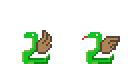
\includegraphics[scale=3]{T08_03}
\centering
\caption{NPC (Amaru)}
Elaborado por: Carlos Acuña
\label{fig:T08_03}
\end{figure}

\begin{figure}[!]
\captionsetup{justification=centering,margin=2cm}
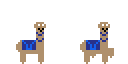
\includegraphics[scale=3]{T08_04}
\centering
\caption{NPC (Jarjacha)}
Elaborado por: Carlos Acuña
\label{fig:T08_04}
\end{figure}
\clearpage
\item \textbf{Animaciones de los enemigos.} Gracias a la herramienta Animator y Animation se puede simular varios movimientos para los enemigos con los sprites creados para este propósito.

\begin{figure}[h]
\captionsetup{justification=centering,margin=2cm}
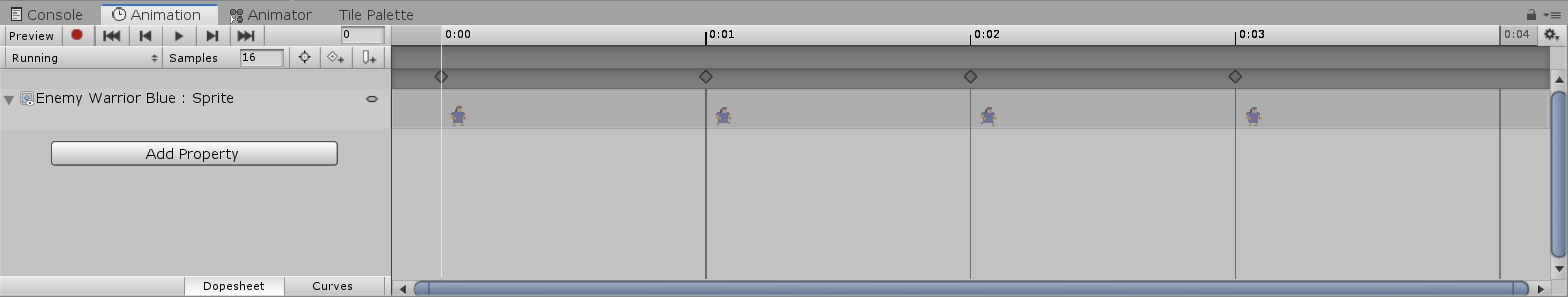
\includegraphics[scale=0.5]{T08_05}
\centering
\caption{Uso de la herramienta Animation para el NPC (Guerrero)}
Elaborado por: Carlos Acuña
\label{fig:T08_05}
\end{figure}

\begin{figure}[h]
\captionsetup{justification=centering,margin=2cm}
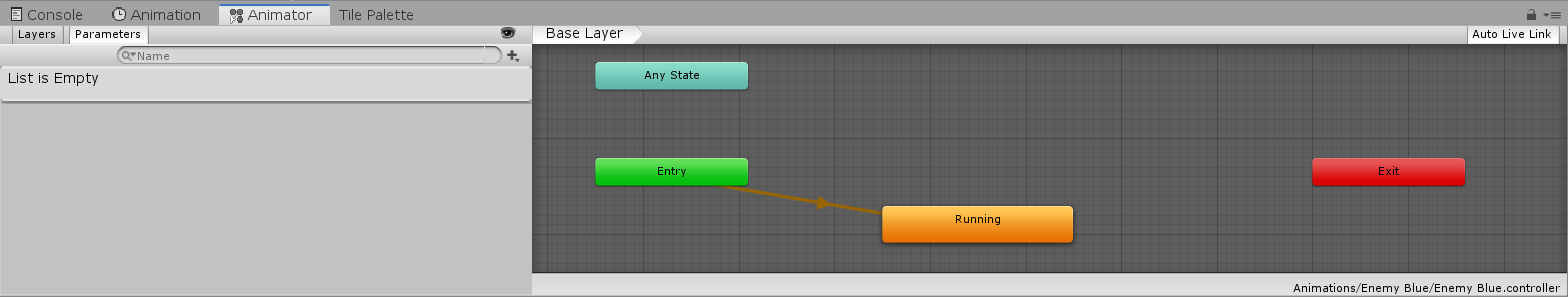
\includegraphics[scale=0.5]{T08_06}
\centering
\caption{Uso de la herramienta Animator para el NPC (Guerrero)}
Elaborado por: Carlos Acuña
\label{fig:T08_06}
\end{figure}

\item \textbf{Creación de la clase ``Enemy.cs".} Para que cada enemigo tenga un comportamiento dentro del juego, se debe crear un script que cumpla esta función, esta clase se llamará ``Enemy.cs", esta clase contendrá varios métodos para el correcto funcionamiento del NPC.

\begin{itemize}
\item \textbf{Movimiento del personaje.} Para que el personaje se mueva de izquierda a derecha y viceversa como si estuviera patrullando se ha generado varios métodos que permiten esta acción. Asi tenemos el método \textbf{``IsFacingRight"} para mostrar al personaje mirando hacia el lado correcto de la pantalla, donde conjuntamente con el método \textbf{``Update"} se permite que realice el movimiento en esa dirección.

\begin{figure}[h]
\captionsetup{justification=centering,margin=2cm}
\centering
\lstset{language=C, breaklines=true, basicstyle=\footnotesize}
\lstset{numbers=left, numberstyle=\tiny, stepnumber=1, numbersep=-2pt}
\captionsetup{justification=centering,margin=2cm}
\begin{lstlisting}[frame=single]
  bool IsFacingRight()
    {
        return transform.localScale.x > 0;
    }
\end{lstlisting}
\caption{Método ``IsFacingRight"}
Elaborado por: Carlos Acuña
\end{figure}

\begin{figure}[h]
\captionsetup{justification=centering,margin=2cm}
\centering
\lstset{language=C, breaklines=true, basicstyle=\footnotesize}
\lstset{numbers=left, numberstyle=\tiny, stepnumber=1, numbersep=-2pt}
\captionsetup{justification=centering,margin=2cm}
\begin{lstlisting}[frame=single]
    void Update()
    {
        if (IsFacingRight())
        {
            myRigidBody.velocity = new Vector2(moveSpeed, 0f);
        }
        else
        {
            myRigidBody.velocity = new Vector2(-moveSpeed, 0f);
        }
    }
\end{lstlisting}
\caption{Método ``Update" para el movimiento del enemigo}
Elaborado por: Carlos Acuña
\end{figure}
\clearpage
\item \textbf{Vida y muerte del personaje.} Todo NPC enemigo tiene cierta cantidad de vida que cuando llega a 0 desaparece del mapa, para lo cual se ha creado dos métodos que permiten realizar esta acción. Así se obtiene el método \textbf{``TakeDamage"} y el método \textbf{``Die"} para cumplir esta tarea.

\begin{figure}[h]
\captionsetup{justification=centering,margin=2cm}
\centering
\lstset{language=C, breaklines=true, basicstyle=\footnotesize}
\lstset{numbers=left, numberstyle=\tiny, stepnumber=1, numbersep=-2pt}
\captionsetup{justification=centering,margin=2cm}
\begin{lstlisting}[frame=single]
    public void TakeDamage(int damage)
    {
        health -= damage;
        if (health <= 0)
        {
            Die();
        }
    }
\end{lstlisting}
\caption{Método ``TakeDamage"}
Elaborado por: Carlos Acuña
\end{figure}

\begin{figure}[h]
\captionsetup{justification=centering,margin=2cm}
\centering
\lstset{language=C, breaklines=true, basicstyle=\footnotesize}
\lstset{numbers=left, numberstyle=\tiny, stepnumber=1, numbersep=-2pt}
\captionsetup{justification=centering,margin=2cm}
\begin{lstlisting}[frame=single]
    private void Die()
    {
        AudioSource.PlayClipAtPoint(hurtSFX, Camera.main.transform.position);
        Destroy(gameObject);
    }
\end{lstlisting}
\caption{Método ``Die"}
Elaborado por: Carlos Acuña
\end{figure}
\end{itemize}
\clearpage
\item \textbf{Destrucción del enemigo.} Cada enemigo debe poder ser eliminado del juego luego de que el jugador realice la acción disparar y el proyectil choque con el NPC. Para esto se ha de añadir algunas reglas a la clase "Projectile.cs". Dentro del método \textbf{``OnTriggerEnter2D"} se creará un evento que detecte la colisión del proyectil con el enemigo y llame al método \textbf{``TakeDamage"} de la clase \textbf{``Enemy.cs"}.

\begin{figure}[h]
\captionsetup{justification=centering,margin=2cm}
\centering
\lstset{language=C, breaklines=true, basicstyle=\footnotesize}
\lstset{numbers=left, numberstyle=\tiny, stepnumber=1, numbersep=-2pt}
\captionsetup{justification=centering,margin=2cm}
\begin{lstlisting}[frame=single]
    private void OnTriggerEnter2D(Collider2D other)
    {
        Enemy enemy = other.GetComponent<Enemy>();
        if (enemy != null)
        {
            enemy.TakeDamage(damage);
            Instantiate(deathExplosion, transform.position, transform.rotation);
            Destroy(gameObject);
        }
    }
\end{lstlisting}
\caption{Método ``OnTriggerEnter2D" de la clase "Projectile.cs"}
Elaborado por: Carlos Acuña
\end{figure}

\end{itemize}

\subsection*{T09: Antes de cada nivel conocer el trasfondo histórico y los personajes principales}
\justify
Para tener un transfondo histórico se debe crear una cinemática que permita saber lo que está pasando en cada nivel, es así como se utiliza el recurso literario de la fantasía histórica para contar una historia que se basa en hechos reales.
Para que esto funcione se debe crear una escena especial que contenga el storyboard y que sea fácil de entender para el jugador.\\
Para realizar esta actividad se debe crear una escena donde el jugador pueda leer una historieta que se cuenta en primera persona del héroe del juego conocido como Huaraca y que se entienda el trasfondo de la historia que sucede en ella. Para ello se deben realizar las siguientes actividades:
\begin{itemize}
\item \textbf{Creación del sistema de diálogos.} Este sistema permite simular una pantalla de diálogo donde el personaje principal cuenta su historia. Para esto se creado una clase llamada \textbf{``Dialogues.cs"}, donde el método \textbf{``Type"} crea un efecto estilizado al momento de mostrar el texto de la historia y además permite cambiar la imagen en cada cambio de frase y el método \textbf{``NextSentence"} que alterna entre el botón continuar y el botón que permite ir al siguiente nivel que está bajo el llamado del método \textbf{``NextLevel"}.

\begin{figure}[!]
\captionsetup{justification=centering,margin=2cm}
\centering
\lstset{language=C, breaklines=true, basicstyle=\footnotesize}
\lstset{numbers=left, numberstyle=\tiny, stepnumber=1, numbersep=-2pt}
\captionsetup{justification=centering,margin=2cm}
\begin{lstlisting}[frame=single]
    IEnumerator Type()
    {
        if (textFile != null)
        {
            sentences = textFile.text.Split('\n');
            foreach (char letter in sentences[index].ToCharArray())
            {
                textDisplay.text += letter;
                storyImage.GetComponent<Image>().sprite = sprites[index];                
                myAudioSource.Play();
                myAudioSource.volume = 0.1f;
                yield return new WaitForSeconds(typingSpeed);
            }
        }
    }
\end{lstlisting}
\caption{Método ``Type"}
Elaborado por: Carlos Acuña
\end{figure}

\begin{figure}[!]
\captionsetup{justification=centering,margin=2cm}
\centering
\lstset{language=C, breaklines=true, basicstyle=\footnotesize}
\lstset{numbers=left, numberstyle=\tiny, stepnumber=1, numbersep=-2pt}
\captionsetup{justification=centering,margin=2cm}
\begin{lstlisting}[frame=single]
    public void NextSentence()
    {
        continueButton.SetActive(false);
        if (index < sentences.Length - 1)
        {
            index++;
            textDisplay.text = "";
            StartCoroutine(Type());
        }
        else
        {
            textDisplay.text = "";
            continueButton.SetActive(false);
            nextLevelButton.SetActive(true);
        }
    }
\end{lstlisting}
\caption{Método ``NextSentence"}
Elaborado por: Carlos Acuña
\end{figure}

\begin{figure}[!]
\captionsetup{justification=centering,margin=2cm}
\centering
\lstset{language=C, breaklines=true, basicstyle=\footnotesize}
\lstset{numbers=left, numberstyle=\tiny, stepnumber=1, numbersep=-2pt}
\captionsetup{justification=centering,margin=2cm}
\begin{lstlisting}[frame=single]
    public void NextLevel()
    {
        var currentSceneIndex = SceneManager.GetActiveScene().buildIndex;
        SceneManager.LoadScene(currentSceneIndex + 1);
    }
\end{lstlisting}
\caption{Método ``NextLevel"}
Elaborado por: Carlos Acuña
\end{figure}

\begin{figure}[!]
\captionsetup{justification=centering,margin=2cm}
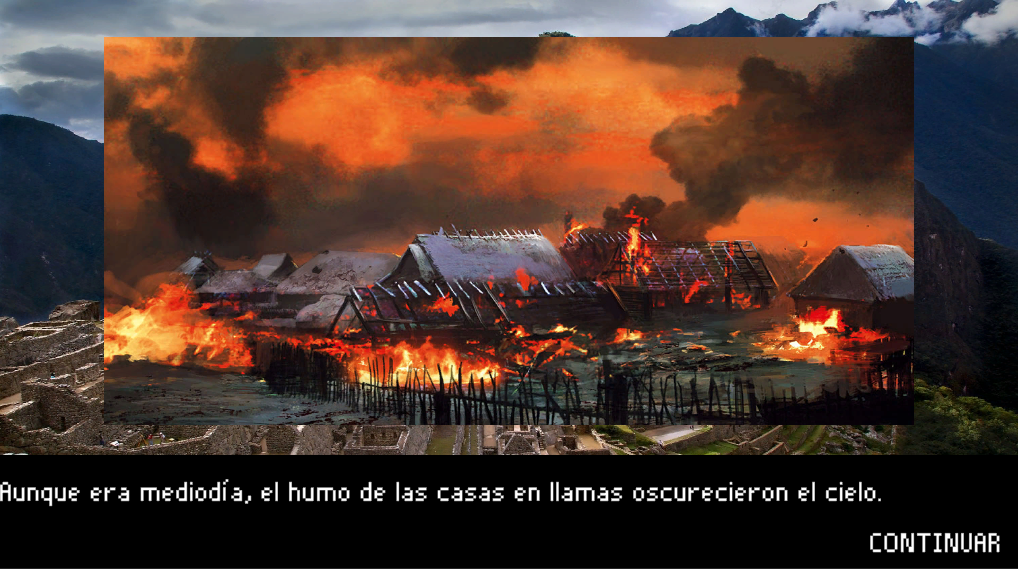
\includegraphics[scale=0.5]{T09_01}
\centering
\caption{Cinemática de la historia dentro del videojuego}
Elaborado por: Carlos Acuña
\label{fig:T09_01}
\end{figure}
  
\end{itemize}  
\clearpage
\subsection*{Entrega funcional de la iteracion 2}
\justify
La segunda iteración para el 17 de febrero del 2020 fue completada con éxito de acuerdo a la planificación que se había planeado.\\
Como resultado se obtuvo que el personaje principal complete su funcionamiento con la acción morir y que las vidas y monedas de oro puedan ser contadas y guardadas en cada nivel. Que cada nivel tenga su contexto histórico y que sirva como medio para presentar el trasfondo del personaje.

\subsection*{Desarrollo de la iteración 3}
\justify
El objetivo de esta iteración es obtener la tercera y última versión del videojuego, la fecha de revisión de la iteración será el día 18 de marzo de 2020, en esta iteración se desarrollará las siguientes historias de usuario.

\begin{longtable}{| l | p{5cm} |}
\hline
\captionsetup{justification=centering,margin=2cm}
\centering
%%Titulo
\textbf{ID} & \textbf{Descripción} \\ \hline
%%Contenido
HU12 &
Visualizar la meta de cada nivel \\ \hline
HU07 &
Al final de cada nivel exista una batalla contra un jefe \\ \hline
HU15 &
Los efectos de sonido sean acordes a las acciones del jugador \\ \hline
HU01 &
Entrar, salir y ver los créditos del juego \\ \hline
HU03 &
Visualizar los controles del juego \\ \hline
HU04 &
Visualizar una pantalla de créditos  \\ \hline
HU05 &
Visualizar una pantalla que cuente el trasfondo histórico del juego\\ \hline 
HU17 &
Agregar un story board en cada cambio de nivel\\ \hline

\caption{Historias de usuario a implementarse en la Iteración 3}
\end{longtable}
\begin{center}
Elaborado por: Carlos Acuña
\end{center}
\subsection*{T10: Visualizar la meta de cada nivel}
\justify
Para visualizar la meta se deben realizar algunos pasos para cumplir con esta tarea:
\begin{itemize}
\item \textbf{Creación de la meta.} Se debe crear un \textbf{``GameObject"} para que pueda interactuar con el jugador y realice un evento dentro del videojuego, la clase que controla estas acciones es la clase \textbf{``LevelExit.cs"}.

\item \textbf{Creación del método ``LoadNextLevel".} Este método permite al jugador saber que terminó el nivel y que puede avanzar en su aventura, además de llevar la información importante como lo es la cantidad de vidas que le sobran al jugador y la cantidad de monedas de oro que tiene. Además genera una pequeña animación con música que permite saber al jugador que ha llegado a la meta. Para que se realice esta acción el jugador debe colisionar con el \textbf{``GameObject"} de la meta y así poder activar el método \textbf{``OnTriggerEnter2D"}.

\begin{figure}[h]
\captionsetup{justification=centering,margin=2cm}
\centering
\lstset{language=C, breaklines=true, basicstyle=\footnotesize}
\lstset{numbers=left, numberstyle=\tiny, stepnumber=1, numbersep=-2pt}
\captionsetup{justification=centering,margin=2cm}
\begin{lstlisting}[frame=single]
    IEnumerator LoadNextLevel()
    {
        Time.timeScale = LevelExitSlowMoFactor;
        levelManager.levelMusic.Stop();
        misionCompletedMusic.Play();
        yield return new WaitForSecondsRealtime(LevelLoadDelay);
        Time.timeScale = 1f;
        PlayerPrefs.SetInt("coinCount", levelManager.coinCount);
        PlayerPrefs.SetInt("playerLives", levelManager.currentLives);
        PlayerPrefs.SetInt(levelToUnlock, 1);
        var currentSceneIndex = SceneManager.GetActiveScene().buildIndex;
        SceneManager.LoadScene(currentSceneIndex + 1);
    }
\end{lstlisting}
\caption{Método ``LoadNextLevel"}
Elaborado por: Carlos Acuña
\end{figure}

\begin{figure}[h]
\lstset{language=C, breaklines=true, basicstyle=\footnotesize}
\lstset{numbers=left, numberstyle=\tiny, stepnumber=1, numbersep=-2pt}
\captionsetup{justification=centering,margin=2cm}
\centering
\begin{lstlisting}[frame=single]
    private void OnTriggerEnter2D(Collider2D other)
    {
        StartCoroutine(LoadNextLevel());
    }
\end{lstlisting}
\caption{Método ``OnTriggerEnter2D" de la clase ``LevelExit.cs"}
Elaborado por: Carlos Acuña
\end{figure}
\end{itemize}

\subsection*{T11: Batalla contra jefe de cada nivel}
En este apartado se ha añadido una batalla contra jefe final, este personaje es diferente del enemigo común ya que tiene más puntos de vida y que se mueve de manera diferente que un enemigo común. Estos personajes aparecen en algunos niveles y ocupan la misma clase \textbf{``Enemy.cs"}, pero se cambian algunos de sus parámetros.

\begin{figure}[!]
\captionsetup{justification=centering,margin=2cm}
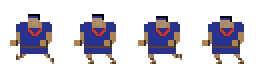
\includegraphics[scale=5]{T11_01}
\centering
\caption{Chapera (Sprites)}
Elaborado por: Carlos Acuña
\label{fig:T11_01}
\end{figure}

\begin{figure}[!]
\captionsetup{justification=centering,margin=2cm}
\includegraphics[scale=5]{T11_02}
\centering
\caption{Apu Atoc (Sprites)}
Elaborado por: Carlos Acuña
\label{fig:T11_02}
\end{figure}

\begin{figure}[!]
\captionsetup{justification=centering,margin=2cm}
\includegraphics[scale=5]{T11_03}
\centering
\caption{Huascar (Sprites)}
Elaborado por: Carlos Acuña
\label{fig:T11_03}
\end{figure}

\subsection*{T12: Los efectos de sonido sean acordes de las acciones del juego}
\justify
Cada vez que se tiene realizar una acción un sonido debe ser utilizado para poder saber que está ocurriendo en el juego, esto se hace mediante un componente de Unity que es \textbf{``AudioSource"} que permite agregar sonidos a los objetos creados y puede ser activado dependiendo de la acción de cada objeto. 

\subsection*{T13: Entrar salir y ver los créditos del juego}
\justify
En esta actividad se crea el menú principal del juego, que permite que el jugador pueda realizar varias acciones relacionadas con la interfaz del videojuego, como jugar, controles, créditos, historia y salir. Estos botones se ven como la figura   \ref{fig:T13_01}

\begin{figure}[h]
\captionsetup{justification=centering,margin=2cm}
\includegraphics[scale=0.5]{T13_01}
\centering
\caption{Pantalla de menú principal}
Elaborado por: Carlos Acuña
\label{fig:T13_01}
\end{figure}

\subsection*{T14: Visualizar los controles del juego}
\justify
En esta pantalla se puede observar los controles del juego mediante una pantalla que muestra al jugador los botones que debe usar para manejar al personaje principal.

\begin{figure}[h]
\captionsetup{justification=centering,margin=2cm}
\includegraphics[scale=0.5]{T14_01}
\centering
\caption{Pantalla de controles}
Elaborado por: Carlos Acuña
\label{fig:T14_01}
\end{figure}

\subsection*{T15: Visualizar los créditos del juego}
\justify
En esta pantalla se observa los créditos de las personas que han creado el juego.

\begin{figure}[h]
\captionsetup{justification=centering,margin=2cm}
\includegraphics[scale=0.5]{T15_01}
\centering
\caption{Pantalla de créditos}
Elaborado por: Carlos Acuña
\label{fig:T15_01}
\end{figure}

\subsection*{T16: Visualizar una pantalla que cuente el trasfondo histórico del juego}
\justify
En esta parte del juego se puede interactuar con una interfaz que permite conocer la historia de cada personaje en la vida real, conocer sus triunfos y derrotas y todo lo relacionado con su vida. En la figura se ve la interfaz donde se muestra una imagen y su respectiva descripción.

\begin{figure}[h]
\captionsetup{justification=centering,margin=2cm}
\includegraphics[scale=0.5]{T16_01}
\centering
\caption{Pantalla de historia}
Elaborado por: Carlos Acuña
\label{fig:T16_01}
\end{figure}

\subsection*{T17: Agregar un story board en cada cambio de nivel}
\justify
El story board solo es las imágenes que se utilizan en la cinemática del videojuego que se puede apreciar en la tarea T09 donde las gráficas son de uso libre y que no exista problemas por derechos de autor.

\subsection*{Entrega funcional de la iteración 3}
\justify
La primera iteración para el 17 de marzo del 2020 fue completada con éxito de acuerdo a la planificación que se había planeado.\\
Como resultado el juego está completamente terminado con todas las especificaciones basadas en las historias de usuarios y correcciones necesarias.

\begin{figure}[h!]
  \centering
  \begin{subfigure}[b]{0.3\linewidth}
    \includegraphics[width=\linewidth]{T13_01}
  \end{subfigure}
  \begin{subfigure}[b]{0.3\linewidth}
    \includegraphics[width=\linewidth]{T14_01}
  \end{subfigure}
  \begin{subfigure}[b]{0.3\linewidth}
    \includegraphics[width=\linewidth]{T15_01}
  \end{subfigure}
  \begin{subfigure}[b]{0.3\linewidth}
    \includegraphics[width=\linewidth]{T16_01}
  \end{subfigure}
  \begin{subfigure}[b]{0.3\linewidth}
    \includegraphics[width=\linewidth]{T17_01}
  \end{subfigure}
  \begin{subfigure}[b]{0.3\linewidth}
    \includegraphics[width=\linewidth]{T18_01}
  \end{subfigure}
  \begin{subfigure}[b]{0.3\linewidth}
    \includegraphics[width=\linewidth]{T19_01}
  \end{subfigure}
  \begin{subfigure}[b]{0.3\linewidth}
    \includegraphics[width=\linewidth]{T20_01}
  \end{subfigure}
  \begin{subfigure}[b]{0.3\linewidth}
    \includegraphics[width=\linewidth]{T21_01}
  \end{subfigure}
  \caption{Capturas del juego ``Huaraca"}
Elaborado por: Carlos Acuña
\label{fig:unity10}
\end{figure}
\clearpage

\subsection{Fase Post-Juego}
\justify
Una vez finalizado con éxito y sin más historias de usuarios que completar se procede a liberar el juego en alguna plataforma virtual con el fin de llegar a una gran cantidad de personas y obtener una retroalimentación como críticas, calificaciones o consejos de todo tipo de personas interesadas en este videojuego.

\subsection*{Evaluación de la tienda online}
Existen muchas tiendas onlines que permiten subir videojuegos de manera gratuita que apoya a desarrolladores independientes ha mostrar sus trabajos y distribuirlos en todo el mundo. De las cuales se ha tomado en cuenta dos tiendas online muy conocidas como son \textbf{``itch.io"} y \textbf{``Gamejolt"}. En el cuadro \ref{t:comparacionTO} se ha comparado varias características para poder escoger la mejor opción basado en los siguientes criterios.

\begin{itemize}
\item \textbf{Pago requerido.} Si es necesario pagar una cantidad para poder subir un videojuego a la plataforma.
\item \textbf{Regalías.} Si la tienda online permite ganar dinero al desarrollador por la venta del videojuego. 
\item \textbf{Multiplataformas.} Permite subir el videojuego para cualquier tipo de plataforma disponible.
\item \textbf{Estadísticas.} Nivel de estadísticas de la plataforma virtual para el desarrollador sobre cómo se está manejando el videojuego.
\end{itemize}

\begin{longtable}{| p{3cm} | p{3cm} | p{3cm}|}
\hline
\captionsetup{justification=centering,margin=2cm}
\centering
%%Titulo
\textbf{} & \textbf{itch.io} & \textbf{Gamejolt}\\ \hline
%%Contenido
Pago requerido 
& No se requiere ningún pago inicial 
& No se requiere ningún pago inicial  
 \\ \hline
Regalías 
& La página permite ganar dinero al desarrollador con un aporte del 10\% a la tienda virtual si el juego se vende. 
& La página permite ganar dinero al desarrollador donde la tienda virtual gana dinero mediante publicidad quedándose con el 70\% de esa ganancia. No hay estas características para Ecuador.
 \\ \hline
Multiplataformas 
& Soporta una gran variedad de plataformas disponibles 
& Soporta una gran variedad de plataformas disponibles  
 \\ \hline
Estadísticas 
& Muestra cantidad de vistas y descargas mensual y anualmente.
& Muestra cantidad de vistas y descargas diario, mensual y anualmente, además de en que plataforma y de que país fue descargado o visto el juego. 
 \\ \hline
\caption{Cuadro comparativo de tiendas online}
\label{t:comparacionTO}
\end{longtable}
\begin{center}
Elaborado por: Carlos Acuña
\end{center}
\justify
Con los resultados obtenidos se ha decidido usar la plataforma Gamejolt porque tiene mejores estadísticas que la plataforma itch.io, lo que beneficia para saber mejor la distribución del juego y conocer mejor la opinión de la gente de este juego.

\subsection*{Publicación en la tienda virtual}
Para publicar en \textbf{``Gamejolt"} se necesita una cuenta con algunas configuraciones para desarrollador y se lo hace de la siguiente manera.
\begin{itemize}
\item \textbf{Añadir juego.} Para añadir un juego se selecciona cualquiera de estos tipos de configuración dependiendo del avance del juego.

\begin{figure}[h]
\captionsetup{justification=centering,margin=2cm}
\includegraphics[scale=0.3]{u01}
\centering
\caption{Sección de añadir juego de Gamejolt}
Elaborado por: Carlos Acuña
\label{fig:u01}
\end{figure}

\item \textbf{Detalle.} En esta ventana se agrega datos básicos del juego.

\begin{figure}[h]
\captionsetup{justification=centering,margin=2cm}
\includegraphics[scale=0.3]{u02}
\centering
\caption{Sección de detalle de Gamejolt}
Elaborado por: Carlos Acuña
\label{fig:u02}
\end{figure}
\clearpage
\item \textbf{Descripción.} En esta sección se agrega una descripción del videojuego.

\begin{figure}[h]
\captionsetup{justification=centering,margin=2cm}
\includegraphics[scale=0.3]{u03}
\centering
\caption{Sección de descripción de Gamejolt}
Elaborado por: Carlos Acuña
\label{fig:u03}
\end{figure}

\item \textbf{Diseño.} En esta sección se agrega varios elementos multimedia para poder mostrar una mejor imagen del videojuego.

\begin{figure}[h]
\captionsetup{justification=centering,margin=2cm}
\includegraphics[scale=0.3]{u04}
\centering
\caption{Sección de diseño de Gamejolt}
Elaborado por: Carlos Acuña
\label{fig:u04}
\end{figure}

\item \textbf{Paquetes.} En esta sección se agrega los paquetes necesarios para que se pueda descargar el videojuego.

\begin{figure}[h]
\captionsetup{justification=centering,margin=2cm}
\includegraphics[scale=0.3]{u05}
\centering
\caption{Sección de paquetes de Gamejolt}
Elaborado por: Carlos Acuña
\label{fig:u05}
\end{figure}
\clearpage
\item \textbf{Madurez.} En esta sección se determina el nivel de madurez que debe tener el jugador para poder jugar el videojuego.

\begin{figure}[h]
\captionsetup{justification=centering,margin=2cm}
\includegraphics[scale=0.3]{u06}
\centering
\caption{Sección de madurez de Gamejolt}
Elaborado por: Carlos Acuña
\label{fig:u06}
\end{figure}

\item \textbf{Preferencia.} En esta sección se determinan algunas preferencias como permitir anuncios, comentarios y calificaciones.

\begin{figure}[h]
\captionsetup{justification=centering,margin=2cm}
\includegraphics[scale=0.3]{u07}
\centering
\caption{Sección de preferencias de Gamejolt}
Elaborado por: Carlos Acuña
\label{fig:u07}
\end{figure}

\justify
Al final se guarda todos los cambios y el juego se publica.
\clearpage
\end{itemize}
\subsection*{Análisis de los resultados de subir el juego a Gamejolt}
\justify
El juego \textbf{``Huaraca"} fue publicado el 20 de marzo de 2020, un mes después se recopila los resultados obtenidos por el videojuego en la página de \textbf{``Gamejolt"} de los cuales se puede obtener el siguiente reporte personalizado.\\
En la figura \ref{fig:u08} se muestra un reporte del total de vistas del juego, el número de descargas, el número de calificaciones y el total de seguidores que tiene el videojuego

\begin{figure}[h]
\captionsetup{justification=centering,margin=2cm}
\includegraphics[scale=1]{u08}
\centering
\caption{Reporte general de Gamejolt}
Elaborado por: Carlos Acuña
\label{fig:u08}
\end{figure}
\justify
El total de vistas por país se muestra en la figura \ref{fig:u09} donde Ecuador destaca con el 95,6\% pero además se halló que hay vistas de otros países como Brasil y Egipto.

\begin{figure}[h]
\captionsetup{justification=centering,margin=2cm}
\includegraphics[scale=1]{u09}
\centering
\caption{Vistas por país del videojuego}
Elaborado por: Carlos Acuña
\label{fig:u09}
\end{figure}

\justify
El número de descargas por país que se muestra en la figura \ref{fig:u10} refleja que el juego tuvo gran aceptación dentro del territorio nacional con un total del 95,45\% de las descargas pero además existe un 4,55\% de descargar realizadas en otros países como es Chile.
\clearpage
\begin{figure}[h]
\captionsetup{justification=centering,margin=2cm}
\includegraphics[scale=1]{u10}
\centering
\caption{Descargas por país del videojuego}
Elaborado por: Carlos Acuña
\label{fig:u10}
\end{figure}

\justify
El sistema operativo destacado para la descarga del juego según la figura \ref{fig:u11} fue other (que puede ser Android) y en segundo lugar fue Windows.

\begin{figure}[h]
\captionsetup{justification=centering,margin=2cm}
\includegraphics[scale=1]{u11}
\centering
\caption{Descargas del videojuego por sistema operativo}
Elaborado por: Carlos Acuña
\label{fig:u11}
\end{figure}
 
\justify
%En el apartado de aceptación del videojuego en la figura \ref{fig:u12} se muestra que a 7 personas le gustó el producto final y dieron una calificación positiva.

%\begin{figure}[h]
%\captionsetup{justification=centering,margin=2cm}
%\includegraphics[scale=1]{u12}
%\centering
%\caption{Descargas del videojuego por sistema operativo\\Elaborado por: Carlos Acuña}
%\label{fig:u12}
%\end{figure}

\justify
Los resultados obtenidos indica una respuesta aceptable pese a ser un juego independiente y sobretodo que el trabajo llegó a un número de personas que viven en el Ecuador, lo que demuestra que a la gente le interesa su cultura y sus tradiciones y que los videojuegos no son ajenos al diario vivir de muchas de estas personas.  

\chapter{Conclusiones y recomendaciones}
\section{Conclusiones}
\begin{itemize}
\item Al utilizar una metodología ágil como DAV, el desarrollo del videojuego tuvo orden y precisión en las tareas que se debe realizar además de agilizar el proceso de creación del proyecto, ya que con todos estos aspectos establecidos se ahorró bastante tiempo y esfuerzo, no hubo necesidad de volver a rehacer el juego  desde el principio y tampoco sucedieron errores fatales durante la creación del mismo. Utilizar este tipo de metodologías ayuda a cualquier desarrollador a enfocarse en una tarea específica y completar el trabajo de la manera más óptima posible. 

\item Encontrar el framework adecuado ayudó a sintetizar las ideas que se tenían sobre la cultura y mitología inca en un videojuego. Al ser una herramienta totalmente nueva, se tiene que dedicar tiempo y esfuerzo en aprender las diferentes técnicas y prácticas de desarrollo correctas para elaborar un producto  de calidad.

\item Elaborar un videojuego sobre un tema como es la cultura y mitología inca fue un reto debido a toda la información que se debe buscar. Transformarla en una historia que sea fácil de entender, utilizar personajes históricos y momentos importantes de la historia que se convirtieron en niveles del videojuego fue una experiencia enriquecedora y compartir esa experiencia a través de este trabajo fue un objetivo que se cumplió al poder publicar el videojuego en una plataforma que llegó a muchas personas interesados en este tipo de temas. 

\item Publicar el videojuego en una plataforma como Gamejolt alienta a desarrolladores independientes a mostrar su trabajo y recibir retroalimentación de la gente para mejorar en todos los aspectos posibles dentro del desarrollo de videojuegos. Este videojuego puede inspirar a otros programadores a realizar sus propios proyectos y compartirlos con la comunidad con el fin de expandir este tipo de desarrollo, además de enseñar sobre una de las culturas más importantes de la antigüedad como es la cultura Inca.
\end{itemize}
\clearpage
\section{Recomendaciones}
\begin{itemize}
\item Para entender mejor el transfondo histórico del juego se puede dirigir a la sección historia donde se encuentra pequeñas cápsulas biográficas de todos los personajes y sucesos históricos que ocurrieron en realidad con el fin de entender mejor la historia y mitología ecuatoriana.

\item El juego fue optimizado para la mayoría de computadoras que corren con windows pero es importante revisar los requerimientos de hardware y software para evitar problemas al momento de correr el juego.

\item Gracias a la página donde fue publicado el videojuego se puede conocer de novedades, actualizaciones y reporte de errores que permiten al desarrollador mejorar el producto para satisfacer las demandas de los seguidores y ofrecer un software de calidad.

\item Con más conocimiento y mejores habilidades en el diseño gráfico se puede pensar en una continuación del juego en una segunda versión, con aumento de héroes, habilidades, jefes de nivel entre otras cosas que pueden enriquecer el juego y contar aún más historias sobre la cultura ecuatoriana en general.
\end{itemize}
\clearpage
\bibliographystyle{unsrt} 
\phantomsection
\addcontentsline{toc}{chapter}{Bibliografía}
\bibliography{biblio}
\clearpage
\appendix
\pagestyle{empty}
\chapter{Tarjetas de tareas}\label{aped.A}

\begin{longtable}{| p{6cm} | p{6cm} |}
\hline
\multicolumn{2}{|c|}{\textbf{Tarjeta de tarea}} \\
\hline
\textbf{Número de tarea:} T01 & \textbf{Historia de Usuario (Nro. y Nombre):} HU08\\
\hline
\multicolumn{2}{|p{12cm}|}{\textbf{Nombre de Tarea:} Reflejar paisajes andinos mediante pixel art} \\ \hline
\textbf{Tipo de tarea:} Diseño & \textbf{Puntos estimados:} 60 horas  \\ \hline
\textbf{Inicio:} 19 de diciembre del 2019 & \textbf{Fin:} 26 diciembre del 2019 \\ \hline
\multicolumn{2}{|p{12cm}|}{\textbf{Miembro responsable:} Carlos Acuña} \\ \hline
\multicolumn{2}{|p{12cm}|}{\textbf{Descripción:} Crear niveles en pixel art} \\ \hline
\end{longtable}

\begin{longtable}{| p{6cm} | p{6cm} |}
\hline
\multicolumn{2}{|c|}{\textbf{Tarjeta de tarea}} \\
\hline
\textbf{Número de tarea:} T02 & \textbf{Historia de Usuario (Nro. y Nombre):} HU11\\
\hline
\multicolumn{2}{|p{12cm}|}{\textbf{Nombre de Tarea:} El personaje principal cambie de animación según su acción} \\ \hline
\textbf{Tipo de tarea:} Diseño & \textbf{Puntos estimados:} 48 horas  \\ \hline
\textbf{Inicio:} 27 de diciembre del 2019 & \textbf{Fin:} 2 de enero del 2020 \\ \hline
\multicolumn{2}{|p{12cm}|}{\textbf{Miembro responsable:} Carlos Acuña} \\ \hline
\multicolumn{2}{|p{12cm}|}{\textbf{Descripción:} Crear las animaciones del personaje principal} \\ \hline
\end{longtable}

\begin{longtable}{| p{6cm} | p{6cm} |}
\hline
\multicolumn{2}{|c|}{\textbf{Tarjeta de tarea}} \\
\hline
\textbf{Número de tarea:} T03 & \textbf{Historia de Usuario (Nro. y Nombre):} HU19\\
\hline
\multicolumn{2}{|p{12cm}|}{\textbf{Nombre de Tarea:} Acciones del personaje} \\ \hline
\textbf{Tipo de tarea:} Desarrollo & \textbf{Puntos estimados:} 36 horas  \\ \hline
\textbf{Inicio:} 3 de enero del 2020 & \textbf{Fin:} 8 de enero del 2020 \\ \hline
\multicolumn{2}{|p{12cm}|}{\textbf{Miembro responsable:} Carlos Acuña} \\ \hline
\multicolumn{2}{|p{12cm}|}{\textbf{Descripción:} Crear acciones que permitan la interacción y progresión del juego} \\ \hline
\end{longtable}

\clearpage

\begin{longtable}{| p{6cm} | p{6cm} |}
\hline
\multicolumn{2}{|c|}{\textbf{Tarjeta de tarea}} \\
\hline
\textbf{Número de tarea:} T04 & \textbf{Historia de Usuario (Nro. y Nombre):} HU10\\
\hline
\multicolumn{2}{|p{12cm}|}{\textbf{Nombre de Tarea:} La cámara sigue al jugador en todo momento} \\ \hline
\textbf{Tipo de tarea:} Desarrollo & \textbf{Puntos estimados:} 36 horas  \\ \hline
\textbf{Inicio:} 9 de enero del 2020 & \textbf{Fin:} 14 de enero del 2020 \\ \hline
\multicolumn{2}{|p{12cm}|}{\textbf{Miembro responsable:} Carlos Acuña} \\ \hline
\multicolumn{2}{|p{12cm}|}{\textbf{Descripción:} Crear evento que permite seguir al personaje principal} \\ \hline
\end{longtable}

\begin{longtable}{| p{6cm} | p{6cm} |}
\hline
\multicolumn{2}{|c|}{\textbf{Tarjeta de tarea}} \\
\hline
\textbf{Número de tarea:} T05 & \textbf{Historia de Usuario (Nro. y Nombre):} HU14\\
\hline
\multicolumn{2}{|p{12cm}|}{\textbf{Nombre de Tarea:} Los niveles tengan un fondo estilo pixel art} \\ \hline
\textbf{Tipo de tarea:} Diseño & \textbf{Puntos estimados:} 24 horas  \\ \hline
\textbf{Inicio:} 15 de enero del 2020 & \textbf{Fin:} 17 de enero del 2020 \\ \hline
\multicolumn{2}{|p{12cm}|}{\textbf{Miembro responsable:} Carlos Acuña} \\ \hline
\multicolumn{2}{|p{12cm}|}{\textbf{Descripción:} Encontrar escenarios que sean pixelart} \\ \hline
\end{longtable}

\begin{longtable}{| p{6cm} | p{6cm} |}
\hline
\multicolumn{2}{|c|}{\textbf{Tarjeta de tarea}} \\
\hline
\textbf{Número de tarea:} T06 & \textbf{Historia de Usuario (Nro. y Nombre):} HU09\\
\hline
\multicolumn{2}{|p{12cm}|}{\textbf{Nombre de Tarea:} Visualizar las vidas
restantes y la puntuación actual} \\ \hline
\textbf{Tipo de tarea:} Desarrollo & \textbf{Puntos estimados:} 48 horas  \\ \hline
\textbf{Inicio:} 20 de enero del 2020 & \textbf{Fin:} 24 de enero del 2020 \\ \hline
\multicolumn{2}{|p{12cm}|}{\textbf{Miembro responsable:} Carlos Acuña} \\ \hline
\multicolumn{2}{|p{12cm}|}{\textbf{Descripción:} Visualizar las vidas
restantes y la puntuación actual del personaje principal} \\ \hline
\end{longtable}

\begin{longtable}{| p{6cm} | p{6cm} |}
\hline
\multicolumn{2}{|c|}{\textbf{Tarjeta de tarea}} \\
\hline
\textbf{Número de tarea:} T07 & \textbf{Historia de Usuario (Nro. y Nombre):} HU13\\
\hline
\multicolumn{2}{|p{12cm}|}{\textbf{Nombre de Tarea:} El personaje pierda el nivel cuando sus vidas lleguen a 0} \\ \hline
\textbf{Tipo de tarea:} Desarrollo & \textbf{Puntos estimados:} 48 horas  \\ \hline
\textbf{Inicio:} 27 de enero del 2020 & \textbf{Fin:} 31 de enero del 2020 \\ \hline
\multicolumn{2}{|p{12cm}|}{\textbf{Miembro responsable:} Carlos Acuña} \\ \hline
\multicolumn{2}{|p{12cm}|}{\textbf{Descripción:} El personaje pierda el nivel cuando sus vidas lleguen a 0 mediante código} \\ \hline
\end{longtable}
\clearpage
\begin{longtable}{| p{6cm} | p{6cm} |}
\hline
\multicolumn{2}{|c|}{\textbf{Tarjeta de tarea}} \\
\hline
\textbf{Número de tarea:} T08 & \textbf{Historia de Usuario (Nro. y Nombre):} HU06\\
\hline
\multicolumn{2}{|p{12cm}|}{\textbf{Nombre de Tarea:} Existan enemigos variados
en cada nivel y puedan ser destruidos} \\ \hline
\textbf{Tipo de tarea:} Desarrollo & \textbf{Puntos estimados:} 48 horas  \\ \hline
\textbf{Inicio:} 3 de febrero del 2020 & \textbf{Fin:} 7 de febrero del 2020 \\ \hline
\multicolumn{2}{|p{12cm}|}{\textbf{Miembro responsable:} Carlos Acuña} \\ \hline
\multicolumn{2}{|p{12cm}|}{\textbf{Descripción:} Creación, animación y codificación de varios enemigos en cada nivel} \\ \hline
\end{longtable}

\begin{longtable}{| p{6cm} | p{6cm} |}
\hline
\multicolumn{2}{|c|}{\textbf{Tarjeta de tarea}} \\
\hline
\textbf{Número de tarea:} T09 & \textbf{Historia de Usuario (Nro. y Nombre):} HU02\\
\hline
\multicolumn{2}{|p{12cm}|}{\textbf{Nombre de Tarea:} Antes de cada nivel conocer
el transfondo histórico y los personajes principales} \\ \hline
\textbf{Tipo de tarea:} Desarrollo & \textbf{Puntos estimados:} 48 horas  \\ \hline
\textbf{Inicio:} 10 de febrero del 2020 & \textbf{Fin:} 14 de febrero del 2020 \\ \hline
\multicolumn{2}{|p{12cm}|}{\textbf{Miembro responsable:} Carlos Acuña} \\ \hline
\multicolumn{2}{|p{12cm}|}{\textbf{Descripción:} Creación, animación y codificación para presentación del nivel y sus personajes históricos} \\ \hline
\end{longtable}

\begin{longtable}{| p{6cm} | p{6cm} |}
\hline
\multicolumn{2}{|c|}{\textbf{Tarjeta de tarea}} \\
\hline
\textbf{Número de tarea:} T10 & \textbf{Historia de Usuario (Nro. y Nombre):} HU12\\
\hline
\multicolumn{2}{|p{12cm}|}{\textbf{Nombre de Tarea:} Visualizar la meta de cada
nivel} \\ \hline
\textbf{Tipo de tarea:} Desarrollo & \textbf{Puntos estimados:} 24 horas  \\ \hline
\textbf{Inicio:} 17 de febrero del 2020 & \textbf{Fin:} 19 de febrero del 2020 \\ \hline
\multicolumn{2}{|p{12cm}|}{\textbf{Miembro responsable:} Carlos Acuña} \\ \hline
\multicolumn{2}{|p{12cm}|}{\textbf{Descripción:} Creación, animación y codificación de la meta de cada nivel} \\ \hline
\end{longtable}

\begin{longtable}{| p{6cm} | p{6cm} |}
\hline
\multicolumn{2}{|c|}{\textbf{Tarjeta de tarea}} \\
\hline
\textbf{Número de tarea:} T11 & \textbf{Historia de Usuario (Nro. y Nombre):} HU07\\
\hline
\multicolumn{2}{|p{12cm}|}{\textbf{Nombre de Tarea:} Al final de cada nivel exista una batalla contra un jefe} \\ \hline
\textbf{Tipo de tarea:} Desarrollo & \textbf{Puntos estimados:} 12 horas  \\ \hline
\textbf{Inicio:} 20 de febrero del 2020 & \textbf{Fin:} 21 de febrero del 2020 \\ \hline
\multicolumn{2}{|p{12cm}|}{\textbf{Miembro responsable:} Carlos Acuña} \\ \hline
\multicolumn{2}{|p{12cm}|}{\textbf{Descripción:} Creación, animación y codificación de la pelea contra jefe de nivel} \\ \hline
\end{longtable}
\clearpage
\begin{longtable}{| p{6cm} | p{6cm} |}
\hline
\multicolumn{2}{|c|}{\textbf{Tarjeta de tarea}} \\
\hline
\textbf{Número de tarea:} T12 & \textbf{Historia de Usuario (Nro. y Nombre):} HU15\\
\hline
\multicolumn{2}{|p{12cm}|}{\textbf{Nombre de Tarea:} Los efectos de sonido sean
acordes a las acciones del jugador} \\ \hline
\textbf{Tipo de tarea:} Desarrollo & \textbf{Puntos estimados:} 24 horas  \\ \hline
\textbf{Inicio:} 24 de febrero del 2020 & \textbf{Fin:} 26 de febrero del 2020 \\ \hline
\multicolumn{2}{|p{12cm}|}{\textbf{Miembro responsable:} Carlos Acuña} \\ \hline
\multicolumn{2}{|p{12cm}|}{\textbf{Descripción:} Búsqueda e implementación del sonido y ambientación al juego} \\ \hline
\end{longtable}

\begin{longtable}{| p{6cm} | p{6cm} |}
\hline
\multicolumn{2}{|c|}{\textbf{Tarjeta de tarea}} \\
\hline
\textbf{Número de tarea:} T13 & \textbf{Historia de Usuario (Nro. y Nombre):} HU01\\
\hline
\multicolumn{2}{|p{12cm}|}{\textbf{Nombre de Tarea:} Entrar, salir y ver los
créditos del juego} \\ \hline
\textbf{Tipo de tarea:} Desarrollo & \textbf{Puntos estimados:} 12 horas  \\ \hline
\textbf{Inicio:} 27 de febrero del 2020 & \textbf{Fin:} 28 de febrero del 2020 \\ \hline
\multicolumn{2}{|p{12cm}|}{\textbf{Miembro responsable:} Carlos Acuña} \\ \hline
\multicolumn{2}{|p{12cm}|}{\textbf{Descripción:} Creación de las interfaces de usuario} \\ \hline
\end{longtable}

\begin{longtable}{| p{6cm} | p{6cm} |}
\hline
\multicolumn{2}{|c|}{\textbf{Tarjeta de tarea}} \\
\hline
\textbf{Número de tarea:} T14 & \textbf{Historia de Usuario (Nro. y Nombre):} HU03\\
\hline
\multicolumn{2}{|p{12cm}|}{\textbf{Nombre de Tarea:} Visualizar los controles del juego} \\ \hline
\textbf{Tipo de tarea:} Desarrollo & \textbf{Puntos estimados:} 24 horas  \\ \hline
\textbf{Inicio:} 2 de marzo del 2020 & \textbf{Fin:} 4 de marzo del 2020 \\ \hline
\multicolumn{2}{|p{12cm}|}{\textbf{Miembro responsable:} Carlos Acuña} \\ \hline
\multicolumn{2}{|p{12cm}|}{\textbf{Descripción:} Visualizar los controles del juego} \\ \hline
\end{longtable}

\begin{longtable}{| p{6cm} | p{6cm} |}
\hline
\multicolumn{2}{|c|}{\textbf{Tarjeta de tarea}} \\
\hline
\textbf{Número de tarea:} T15 & \textbf{Historia de Usuario (Nro. y Nombre):} HU04\\
\hline
\multicolumn{2}{|p{12cm}|}{\textbf{Nombre de Tarea:} Visualizar los controles del juego} \\ \hline
\textbf{Tipo de tarea:} Desarrollo & \textbf{Puntos estimados:} 12 horas  \\ \hline
\textbf{Inicio:} 5 de marzo del 2020 & \textbf{Fin:} 6 de marzo del 2020 \\ \hline
\multicolumn{2}{|p{12cm}|}{\textbf{Miembro responsable:} Carlos Acuña} \\ \hline
\multicolumn{2}{|p{12cm}|}{\textbf{Descripción:} Visualizar los controles del juego} \\ \hline
\end{longtable}
\clearpage
\begin{longtable}{| p{6cm} | p{6cm} |}
\hline
\multicolumn{2}{|c|}{\textbf{Tarjeta de tarea}} \\
\hline
\textbf{Número de tarea:} T16 & \textbf{Historia de Usuario (Nro. y Nombre):} HU05\\
\hline
\multicolumn{2}{|p{12cm}|}{\textbf{Nombre de Tarea:} Visualizar una pantalla que
cuente el trasfondo histórico del juego} \\ \hline
\textbf{Tipo de tarea:} Desarrollo & \textbf{Puntos estimados:} 24 horas  \\ \hline
\textbf{Inicio:} 9 de marzo del 2020 & \textbf{Fin:} 11 de marzo del 2020 \\ \hline
\multicolumn{2}{|p{12cm}|}{\textbf{Miembro responsable:} Carlos Acuña} \\ \hline
\multicolumn{2}{|p{12cm}|}{\textbf{Descripción:} Visualizar una pantalla que
cuente el trasfondo histórico del juego} \\ \hline
\end{longtable}

\begin{longtable}{| p{6cm} | p{6cm} |}
\hline
\multicolumn{2}{|c|}{\textbf{Tarjeta de tarea}} \\
\hline
\textbf{Número de tarea:} T17 & \textbf{Historia de Usuario (Nro. y Nombre):} HU17\\
\hline
\multicolumn{2}{|p{12cm}|}{\textbf{Nombre de Tarea:} Agregar un story board en
cada cambio de nivel} \\ \hline
\textbf{Tipo de tarea:} Desarrollo & \textbf{Puntos estimados:} 24 horas  \\ \hline
\textbf{Inicio:} 12 de marzo del 2020 & \textbf{Fin:} 13 de marzo del 2020 \\ \hline
\multicolumn{2}{|p{12cm}|}{\textbf{Miembro responsable:} Carlos Acuña} \\ \hline
\multicolumn{2}{|p{12cm}|}{\textbf{Descripción:} Agregar un story board en
cada cambio de nivel} \\ \hline
\end{longtable}

\thispagestyle{empty}

\end{document}
